%
%  PyMC User's Guide for submission to the Journal of Statistical Software
%
%  Created by Chris Fonnesbeck on 2008-11-12.
%  Copyright (c) 2008 . All rights reserved.
%
\documentclass[]{jss_mod}

% \usepackage{python}
\usepackage{underscore} 
\usepackage{epsfig}
\usepackage{amsmath}
\usepackage{boxedminipage}

\author{Anand Patil\\University of Oxford \And
        David Huard\\McGill University  \And
		Christopher J. Fonnesbeck\\Vanderbilt University}

\title{\pkg{PyMC} : Bayesian Stochastic Modelling in \proglang{Python}}

\Address{
  Anand Patil\\
  Malaria Atlas Project\\
  University of Oxford\\
  Oxford, United Kingdom\\
  E-mail: \email{anand.prabhakar.patil@gmail.com}
  \\

  David Huard \\
  Atmospheric and Oceanic Sciences \\
  McGill University \\
  Montr\'eal, Canada \\
  E-mail: \email{david.huard@gmail.com}\\
  \\
  Christopher J. Fonnesbeck\\
  Department of Biostatistics\\
  School of Medicine\\
  Vanderbilt University\\
  Nashville, TN, USA\\
  E-mail: \email{fonnesbeck@gmail.com}\\
}



%% for pretty printing and a nice hypersummary also set:
\Plainauthor{Anand Patil, David Huard, Christopher Fonnesbeck} %% comma-separated
\Plaintitle{PyMC 2: Bayesian Stochastic Modelling in Python} %% without formatting
\Shorttitle{PyMC 2} %% a short title (if necessary)

\Abstract{
This user guide describes a \proglang{Python} package, \pkg{PyMC}, that allows users to
efficiently code a probabilistic model and draw samples from its
posterior distribution using Markov-Chain Monte Carlo techniques.
}
\Keywords{Bayesian modeling, Markov chain Monte Carlo, simulation, \proglang{Python}}
\Plainkeywords{Bayesian modeling, Markov chain Monte Carlo, simulation, Python}

%% publication information
%% NOTE: Typically, this can be left commented and will be filled out by the technical editor
%% \Volume{13}
%% \Issue{9}
%% \Month{September}
%% \Year{2004}
%% \Submitdate{2004-09-29}
%% \Acceptdate{2004-09-29}

%%%%%%%%%%%%%%% Commands from rst2latex %%%%%%%%%%%%%%%%%%%%%%%%
% These are used in the tex files generated by rst2latex, namely
% README, INSTALL and database
\newcommand{\rubric}[1]{\subsection*{~\hfill {\it #1} \hfill ~}}
\newcommand{\titlereference}[1]{\textsl{#1}}
\newlength{\locallinewidth}
\setlength{\locallinewidth}{7in}
\newlength{\admonitionwidth}
\setlength{\admonitionwidth}{0.9\textwidth}
%%%%%%%%%%%%%%%%%%%%%%%%%%%%%%%%%%%%%%%%%%%%%%%%%%%%%%%%%%%%%%%%%

% The tex files use constructs from the python.sty style file,
% such as \module and \code. The problem is that many commands
% defined in python.sty are also defined in jss.sty, creating
% clashes. In other words, jss is not compatible with python.
% I created a jss_mod.cls file and commented out conflicting
% part of python.sty.

\graphicspath{{../figs/}}
\setcounter{secnumdepth}{2}
\setcounter{tocdepth}{2}
\begin{document}

\maketitle

% Referees suggested adding a table of contents. Is this compatible with JSS
% editorial style ?
% \tableofcontents
\cleardoublepage
\pagenumbering{arabic}

%\linenumbers
\section[Introduction]{Introduction}
\label{chap:intro}
\


\section[Installation]{Installation}
\label{chap:install}
\


\section[Tutorial]{Tutorial}
\label{chap:tutorial}

This tutorial will guide you through a typical \pkg{PyMC} application.
Familiarity with \proglang{Python} is assumed, so if you are new to \proglang{Python}, books such as
\citet{Lutz:2007} or \citet{Langtangen:2009} are the place to start. Plenty of
online documentation can also be found on the
\href{http://www.python.org/doc/}{\proglang{Python} documentation} page.

\subsection{An example statistical model}
Consider the following dataset, which is a time series of recorded coal mining
disasters in the UK from 1851 to 1962 \citep{Jarrett:1979fr}.
\begin{center}
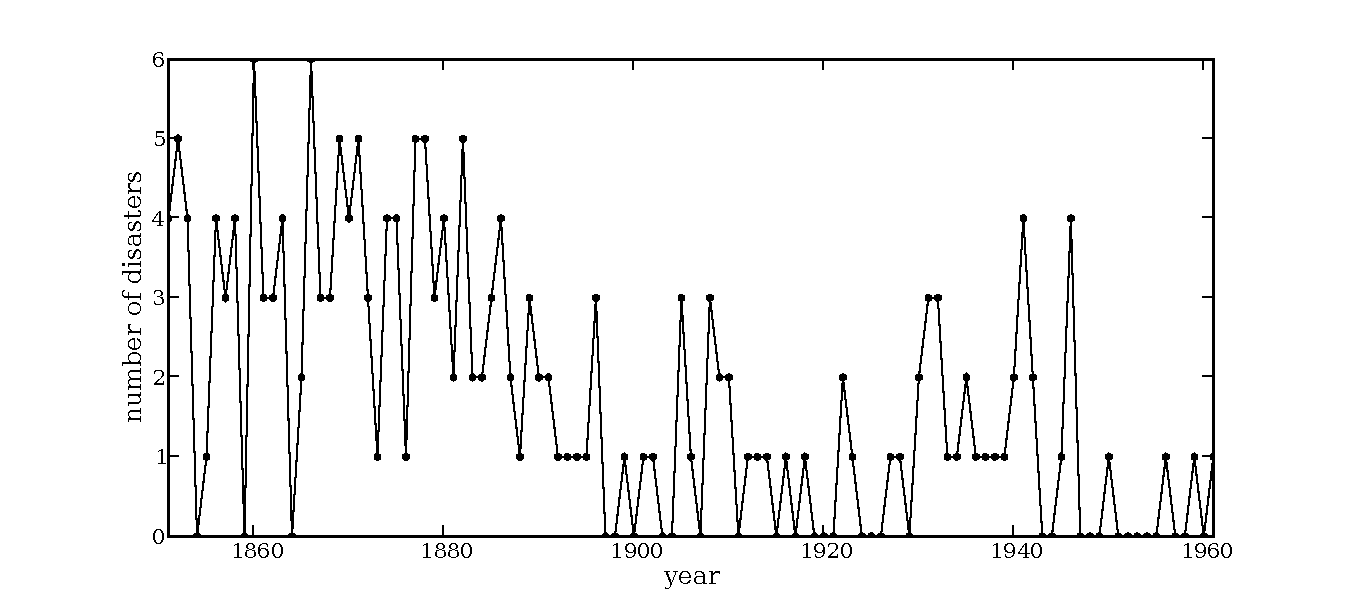
\epsfig{file=disasterts.pdf, width=15cm}
\end{center}
Occurrences of disasters in the time series is thought to be derived from a Poisson process with a large rate parameter in the early part of the time series, and from one with a smaller rate in the later part. We are interested in locating the change point in the series, which perhaps is related to changes in mining safety regulations.

We represent our conceptual model formally as a statistical model:
\begin{equation}
    \begin{array}{ccc}
        (D_t | s, e, l) \sim \textup{Poisson}\left(r_t\right), & r_t=\left\{\begin{array}{lll}
            e &\textup{if}& t< s\\ l &\textup{if}& t\ge s
            \end{array}\right.,&t\in[t_l,t_h]\\
        s\sim \textup{Discrete Uniform}(t_l, t_h)\\
        e\sim \textup{Exponential}(r_e)\\
        l\sim \textup{Exponential}(r_l)
    \end{array}
    \label{disastermodel}
\end{equation}
The symbols are defined as:
\begin{description}
    \item[$D_t$:] The number of disasters in year $t$.
    \item[$r_t$:] The rate parameter of the Poisson distribution of disasters in year $t$.
    \item[$s$:] The year in which the rate parameter changes (the switchpoint).
    \item[$e$:] The rate parameter before the switchpoint $s$.
    \item[$l$:] The rate parameter after the switchpoint $s$.
    \item[$t_l$, $t_h$:] The lower and upper boundaries of year $t$.
    \item[$r_e$, $r_l$:] The rate parameters of the priors of the early and late rates, respectively.
    %\item[$\beta_e$, $\beta_l$:] Prior parameters (also called hyperparameters).
\end{description}
Because we have defined $D$ by its dependence on $s$, $e$ and $l$, the latter three are known as the `parents' of $D$ and $D$ is called their `child'. Similarly, the parents of $s$ are $t_l$ and $t_h$, and $s$ is the child of $t_l$ and $t_h$.


\subsection{Two types of variables}

At the model-specification stage (before the data are observed), $D$, $s$, $e$,
$r$ and $l$ are all random variables. Bayesian `random' variables have not
necessarily arisen from a physical random process. The Bayesian interpretation
of probability is \emph{epistemic}, meaning random variable $x$'s probability
distribution $p(x)$ represents our knowledge and uncertainty about $x$'s value
\citep{jaynes}. Candidate values of $x$ for which $p(x)$ is high are
relatively more probable, given what we know. Random variables are represented
in \pkg{PyMC} by the classes \code{Stochastic} and \code{Deterministic}.

The only \code{Deterministic} in the model is $r$. If we knew the values of
$r$'s parents ($s$, $l$ and $e$), we could compute the value of $r$ exactly. A
\code{Deterministic} like $r$ is defined by a mathematical function that returns
its value given values for its parents. \code{Deterministic} variables are
sometimes called the \emph{systemic} part of the model. The nomenclature is a
bit confusing, because these objects usually represent random variables; since
the parents of $r$ are random, $r$ is random also. A more descriptive (though
more awkward) name for this class would be \code{DeterminedByValuesOfParents}.

On the other hand, even if the values of the parents of variables $s$, $D$ (before observing the data), $e$ or $l$ were known, we would still be uncertain of their values. These variables are characterized by probability distributions that express how plausible their candidate values are, given values for their parents. The \code{Stochastic} class represents these variables. A more descriptive name for these objects might be \code{RandomEvenGivenValuesOfParents}.

We can represent model \ref{disastermodel} in a file called
\code{DisasterModel.py} (the actual file can be found in
\code{pymc/examples/}) as follows. First, we import the \pkg{PyMC} and \pkg{NumPy}
namespaces:
\begin{CodeInput}
\begin{CodeChunk}
	from pymc import DiscreteUniform, Exponential, deterministic, Poisson, Uniform
	import numpy as np
\end{CodeChunk}
\end{CodeInput}
Notice that from \code{pymc} we have only imported a select few objects that are needed for this particular model, whereas the entire \code{numpy} namespace has been imported, and conveniently given a shorter name. Objects from \pkg{NumPy} are subsequently accessed by prefixing \code{np.} to the name. Either approach is acceptable.

Next, we enter the actual data values into an array:
\begin{CodeInput}
\begin{CodeChunk}
	disasters_array =   numpy.array([ 4, 5, 4, 0, 1, 4, 3, 4, 0, 6, 3, 3, 4, 0, 2, 6,
	                   3, 3, 5, 4, 5, 3, 1, 4, 4, 1, 5, 5, 3, 4, 2, 5,
	                   2, 2, 3, 4, 2, 1, 3, 2, 2, 1, 1, 1, 1, 3, 0, 0,
	                   1, 0, 1, 1, 0, 0, 3, 1, 0, 3, 2, 2, 0, 1, 1, 1,
	                   0, 1, 0, 1, 0, 0, 0, 2, 1, 0, 0, 0, 1, 1, 0, 2,
	                   3, 3, 1, 1, 2, 1, 1, 1, 1, 2, 4, 2, 0, 0, 1, 4,
	                   0, 0, 0, 1, 0, 0, 0, 0, 0, 1, 0, 0, 1, 0, 1])
\end{CodeChunk}
\end{CodeInput}
Note that you don't have to type in this entire array to follow along; the code is available in the source tree, in \code{pymc/examples/DisasterModel.py}.  Next, we create the switchpoint variable $s$:
\begin{CodeInput}
\begin{CodeChunk}
	s = DiscreteUniform('s', lower=0, upper=110, doc='Switchpoint[year]')
\end{CodeChunk}
\end{CodeInput}
\code{DiscreteUniform} is a subclass of \code{Stochastic} that represents uniformly-distributed discrete variables. Use of this distribution suggests that we have no preference \emph{a priori} regarding the location of the switchpoint; all values are equally likely. Now we create the exponentially-distributed variables $e$ and $l$ for the early and late Poisson rates, respectively:
\begin{CodeInput}
\begin{CodeChunk}
	e = Exponential('e', beta=1)
	l = Exponential('l', beta=1)
\end{CodeChunk}
\end{CodeInput}
Next, we define the variable $r$, which selects the early rate $e$ for times before $s$ and the late rate $l$ for times after $s$. We create $r$ using the \code{deterministic} decorator, which converts the ordinary \proglang{Python} function $r$ into a \code{Deterministic} object.
\begin{CodeInput}
\begin{CodeChunk}
	@deterministic(plot=False)
	def r(s=s, e=e, l=l):
		""" Concatenate Poisson means """
	    out = numpy.empty(len(disasters_array))
	    out[:s] = e
	    out[s:] = l
	    return out
\end{CodeChunk}
\end{CodeInput}
The last step is to define the number of disasters $D$. This is a stochastic variable, but unlike $s$, $e$ and $l$ we have observed its value. To express this, we set the argument \code{observed} to \code{True} (it is set to \code{False} by default). This tells \pkg{PyMC} that this object's value should not be changed:
\begin{CodeInput}
\begin{CodeChunk}
	D = Poisson('D', mu=r, value=disasters_array, observed=True)
\end{CodeChunk}
\end{CodeInput}

\subsubsection\*{Why are data and unknown variables represented by the same
object?}
Since its represented by a \code{Stochastic} object, $D$ is defined by its dependence on its parent $r$ even though its value is fixed. This isn't just a quirk of \pkg{PyMC}'s syntax; Bayesian hierarchical notation itself makes no distinction between random variables and data. The reason is simple: to use Bayes' theorem to compute the posterior $p(e,s,l|D)$ of model \ref{disastermodel}, we require the likelihood $p(D|e,s,l)$. Even though $D$'s value is known and fixed, we need to formally assign it a probability distribution as if it were a random variable. Remember, the likelihood and the probability function are essentially the same, except that the former is regarded as a function of the parameters and the latter as a function of the data.

This point can be counterintuitive at first, as many peoples' instinct is to regard data as fixed a priori and unknown variables as dependent on the data. One way to understand this is to think of statistical models like (\ref{disastermodel}) as predictive models for data, or as models of the processes that gave rise to data. Before observing the value of $D$, we could have sampled from its prior predictive distribution $p(D)$ (\emph{i.e.} the marginal distribution of the data) as follows:
\begin{enumerate}
    \item Sample $e$, $s$ and $l$ from their priors.
    \item Sample $D$ conditional on these values.
\end{enumerate}
Even after we observe the value of $D$, we need to use this process model to make inferences about $e$, $s$ and $l$ because its the only information we have about how the variables are related.

% ==================================
% = Does this Section~really help? =
% ==================================
% \medskip
% To look at the issue another way, we could, in principle, have written a model equivalent to (\ref{disastermodel}) such that $D$ depended on nothing and everything else depended on $D$, for example
% \begin{eqnarray*}
%     s|e,l,D\sim\cdot\\
%     e|l,D\sim\cdot\\
%     l|D\sim\cdot\\
%     D=D_*
% \end{eqnarray*}
%
% In one respect, this would have been more natural because we would have the unknown stochastic variables depending on the data. However, if we could write down that model using standard distributions we could trivially compute and sample from the posterior,
% \begin{eqnarray*}
%     p(s,e,l|D) = p(s|e, l, D) p(e|l, D) p(l|D),
% \end{eqnarray*}
% and we would have no use for MCMC or any other fitting method. Bayesian methods, and statistics in general, are needed when it's feasible to write down the data's dependence on the unknown variables but not vice versa.


\subsection{Parents and children}

We have above created a \pkg{PyMC} probability model, which is simply a linked collection of variables. To see the nature of the links, import or run \code{DisasterModel.py} and examine $s$'s \code{parents} attribute from the \proglang{Python} prompt:
\begin{CodeInput}
\begin{CodeChunk}
   >>> from pymc.examples import DisasterModel
   >>> DisasterModel.s.parents
   {'lower': 0, 'upper': 110}
\end{CodeChunk}
\end{CodeInput}
The \code{parents} dictionary shows us the distributional parameters of $s$, which are constants. Now let's examinine $D$'s parents:
\begin{CodeInput}
\begin{CodeChunk}
   >>> DisasterModel.D.parents
   {'mu': <pymc.\pkg{PyMC}Objects.Deterministic 'r' at 0x3e51a70>}
\end{CodeChunk}
\end{CodeInput}
We are using $r$ as a distributional parameter of $D$ (\emph{i.e.} $r$ is $D$'s parent). $D$ internally labels $r$ as \code{mu}, meaning $r$ plays the role of the rate parameter in $D$'s Poisson distribution. Now examine $r$'s \code{children} attribute:
\begin{CodeInput}
\begin{CodeChunk}
   >>> DisasterModel.r.children
   set([<pymc.distributions.Poisson 'D' at 0x3e51290>])
\end{CodeChunk}
\end{CodeInput}
Because $D$ considers $r$ its parent, $r$ considers $D$ its child. Unlike \code{parents}, \code{children} is a set (an unordered collection of objects); variables do not associate their children with any particular distributional role. Try examining the \code{parents} and \code{children} attributes of the other parameters in the model.

The following `directed acyclic graph' is a visualization of the parent-child relationships in the model. Unobserved stochastic variables $s$, $e$ and $l$ are open ellipses, observed stochastic variable $D$ is a filled ellipse and deterministic variable $r$ is a triangle. Arrows point from parent to child and display the label that the child assigns to the parent. See Section~\ref{graphical} for more details.
\begin{center}
   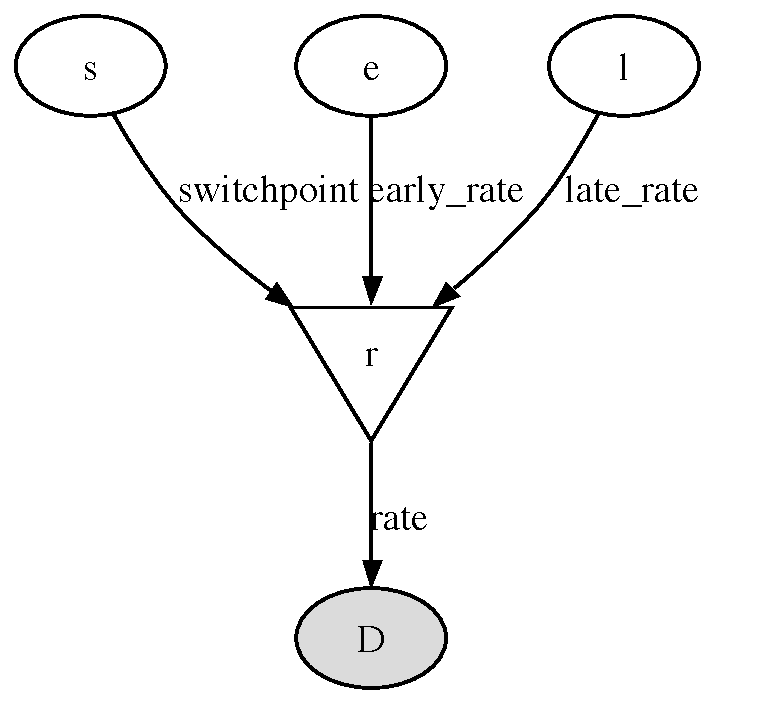
\epsfig{file=DisasterModel2.pdf, width=5cm}
\end{center}


\begin{center}
\begin{sffamily}
\fbox{\parbox{\admonitionwidth}{
\textbf{\large Objects and names}
\vspace{2mm}
As the examples above have shown, pymc objects need to have a name 
assigned, such as \emph{lower}, \emph{upper} or \emph{e}. These names 
are used for storage and post-processing:
\begin{itemize}
 \item as keys in on-disk databases,
 \item as node labels in model graphs,
 \item as axis labels in plots of traces, 
 \item as table labels in summary statistics. 
\end{itemize}
A model instantiated with variables having identical names raises an
error to avoid name conflicts in the database storing the traces. In
general however, pymc uses references to the objects themselves, not 
their names, to identify variables. 
}}
\end{sffamily}
\end{center}



\subsection{Variables' values and log-probabilities}
All \pkg{PyMC} variables have an attribute called \code{value} that stores the current value of that variable. Try examining $D$'s value, and you'll see the initial value we provided for it:
\begin{CodeInput}
\begin{CodeChunk}
   >>> DisasterModel.D.value
   array([4, 5, 4, 0, 1, 4, 3, 4, 0, 6, 3, 3, 4, 0, 2, 6, 3, 3, 5, 4, 5, 3, 1,
          4, 4, 1, 5, 5, 3, 4, 2, 5, 2, 2, 3, 4, 2, 1, 3, 2, 2, 1, 1, 1, 1, 3,
          0, 0, 1, 0, 1, 1, 0, 0, 3, 1, 0, 3, 2, 2, 0, 1, 1, 1, 0, 1, 0, 1, 0,
          0, 0, 2, 1, 0, 0, 0, 1, 1, 0, 2, 3, 3, 1, 1, 2, 1, 1, 1, 1, 2, 4, 2,
          0, 0, 1, 4, 0, 0, 0, 1, 0, 0, 0, 0, 0, 1, 0, 0, 1, 0, 1])
\end{CodeChunk}
\end{CodeInput}
If you check $e$'s, $s$'s and $l$'s values, you'll see random initial values generated by \pkg{PyMC}:
\begin{CodeInput}
\begin{CodeChunk}
   >>> DisasterModel.s.value
   44

   >>> DisasterModel.e.value
   0.33464706250079584

   >>> DisasterModel.l.value
   2.6491936762267811
\end{CodeChunk}
\end{CodeInput}
Of course, since these are \code{Stochastic} elements, your values will be different than these. If you check $r$'s value, you'll see an array whose first $s$ elements are $e$ (here 0.33464706), and whose remaining elements are $l$ (here 2.64919368):
\begin{CodeInput}
\begin{CodeChunk}
   >>> DisasterModel.r.value
   array([ 0.33464706,  0.33464706,  0.33464706,  0.33464706,  0.33464706,
           0.33464706,  0.33464706,  0.33464706,  0.33464706,  0.33464706,
           0.33464706,  0.33464706,  0.33464706,  0.33464706,  0.33464706,
           0.33464706,  0.33464706,  0.33464706,  0.33464706,  0.33464706,
           0.33464706,  0.33464706,  0.33464706,  0.33464706,  0.33464706,
           0.33464706,  0.33464706,  0.33464706,  0.33464706,  0.33464706,
           0.33464706,  0.33464706,  0.33464706,  0.33464706,  0.33464706,
           0.33464706,  0.33464706,  0.33464706,  0.33464706,  0.33464706,
           0.33464706,  0.33464706,  0.33464706,  0.33464706,  2.64919368,
           2.64919368,  2.64919368,  2.64919368,  2.64919368,  2.64919368,
           2.64919368,  2.64919368,  2.64919368,  2.64919368,  2.64919368,
           2.64919368,  2.64919368,  2.64919368,  2.64919368,  2.64919368,
           2.64919368,  2.64919368,  2.64919368,  2.64919368,  2.64919368,
           2.64919368,  2.64919368,  2.64919368,  2.64919368,  2.64919368,
           2.64919368,  2.64919368,  2.64919368,  2.64919368,  2.64919368,
           2.64919368,  2.64919368,  2.64919368,  2.64919368,  2.64919368,
           2.64919368,  2.64919368,  2.64919368,  2.64919368,  2.64919368,
           2.64919368,  2.64919368,  2.64919368,  2.64919368,  2.64919368,
           2.64919368,  2.64919368,  2.64919368,  2.64919368,  2.64919368,
           2.64919368,  2.64919368,  2.64919368,  2.64919368,  2.64919368,
           2.64919368,  2.64919368,  2.64919368,  2.64919368,  2.64919368,
           2.64919368,  2.64919368,  2.64919368,  2.64919368,  2.64919368])
\end{CodeChunk}
\end{CodeInput}
To compute its value, $r$ calls the funtion we used to create it, passing in the values of its parents.

\code{Stochastic} objects can evaluate their probability mass or density functions at their current values given the values of their parents. The logarithm of a stochastic object's probability mass or density can be accessed via the \code{logp} attribute. For vector-valued variables like $D$, the \code{logp} attribute returns the sum of the logarithms of the joint probability or density of all elements of the value. Try examining $s$'s and $D$'s log-probabilities and $e$'s and $l$'s log-densities:
\begin{CodeInput}
\begin{CodeChunk}
   >>> DisasterModel.s.logp
   -4.7095302013123339

   >>> DisasterModel.D.logp
   -1080.5149888046033

   >>> DisasterModel.e.logp
   -0.33464706250079584

   >>> DisasterModel.l.logp
   -2.6491936762267811
\end{CodeChunk}
\end{CodeInput}
\code{Stochastic} objects need to call an internal function to compute their \code{logp} attributes, as $r$ needed to call an internal function to compute its value. Just as we created $r$ by decorating a function that computes its value, it's possible to create custom \code{Stochastic} objects by decorating functions that compute their log-probabilities or densities (see Section~\ref{chap:modelbuilding}). Users are thus not limited to the set of of statistical distributions provided by \pkg{PyMC}.

\subsubsection\*[Using Variables as parents of other Variables]{Using
\code{Variables} as parents of other \code{Variables}}

Let's take a closer look at our definition of $r$:
\begin{CodeInput}
\begin{CodeChunk}
	@deterministic(plot=False)
	def r(s=s, e=e, l=l):
	    """ Concatenate Poisson means """
	    out = numpy.empty(len(disasters_array))
	    out[:s] = e
	    out[s:] = l
	    return out
\end{CodeChunk}
\end{CodeInput}
The arguments $s$, $e$ and $l$ are \code{Stochastic} objects, not numbers. Why aren't errors raised when we attempt to slice array \code{out} up to a \code{Stochastic} object?

Whenever a variable is used as a parent for a child variable, \pkg{PyMC} replaces it with its \code{value} attribute when the child's value or log-probability is computed. When $r$'s value is recomputed, \code{s.value} is passed to the function as argument \code{s}. To see the values of the parents of $r$ all together, look at \code{r.parents.value}.

\subsection{Fitting the model with MCMC}

\pkg{PyMC} provides several objects that fit probability models (linked collections of variables) like ours. The primary such object, \code{MCMC}, fits models with the Markov chain Monte Carlo algorithm \cite{Gamerman:1997tb}. To create an \code{MCMC} object to handle our model, import \code{DisasterModel.py} and use it as an argument for \code{MCMC}:
\begin{CodeInput}
\begin{CodeChunk}
   >>> from pymc.examples import DisasterModel
   >>> from pymc import MCMC
   >>> M = MCMC(DisasterModel)
\end{CodeChunk}
\end{CodeInput}
In this case \code{M} will expose variables \code{s}, \code{e}, \code{l}, \code{r} and \code{D} as attributes; that is, \code{M.s} will be the same object as \code{DisasterModel.s}.

To run the sampler, call the MCMC object's \code{isample()} (or \code{sample()}) method with arguments for the number of iterations, burn-in length, and thinning interval (if desired):
\begin{CodeInput}
\begin{CodeChunk}
   >>> M.isample(iter=10000, burn=1000, thin=10)
\end{CodeChunk}
\end{CodeInput}
After a few seconds, you should see that sampling has finished normally. The model has been fitted.

\subsubsection\*{What does it mean to fit a model?}

`Fitting' a model means characterizing its posterior distribution somehow. In this case, we are trying to represent the posterior $p(s,e,l|D)$ by a set of joint samples from it. To produce these samples, the MCMC sampler randomly updates the values of $s$, $e$ and $l$ according to the Metropolis-Hastings algorithm (\cite{gelman}) for \code{iter}  iterations.

As the number of samples tends to infinity, the MCMC distribution of $s$, $e$
and $l$ converges to the stationary distribution. In other words, their
values can be considered as random draws from the posterior $p(s,e,l|D)$.
\pkg{PyMC} assumes that the \code{burn} parameter specifies a `sufficiently large'
number of iterations for convergence of the algorithm, so it is up to the user
to verify
that this is the case (see Section~\ref{chap:modelchecking}). Consecutive values
sampled from $s$, $e$ and $l$ are necessarily dependent on the previous sample,
since it is a Markov chain. However, MCMC often results in strong
autocorrelation among samples that can result in imprecise posterior inference.
To circumvent this, it is often effective to thin the sample by only retaining
every $k$th sample, where $k$ is an integer value. This thinning interval is
passed to the sampler via the \code{thin} argument.

If you are not sure ahead of time what values to choose for the \code{burn} and \code{thin} parameters, you may want to retain all the MCMC samples, that is to set \code{burn=0} and \code{thin=1}, and then discard the `burnin period' and thin the samples after examining the traces (the series of samples). See \cite{gelman} for general guidance.

\subsubsection\*{Accessing the samples}
The output of the MCMC algorithm is a `trace', the sequence of retained
samples for each variable in the model. These traces can be accessed
using the \code{trace(name, chain=-1)} method. For example:
\begin{CodeInput}
\begin{CodeChunk}
   >>> M.trace('s')[:]
   array([41, 40, 40, ..., 43, 44, 44])
\end{CodeChunk}
\end{CodeInput}
The trace slice \code{[start:stop:step]} works just like the \pkg{NumPy} array
slice. By default, the returned trace array contains the samples from the
last call to \code{sample}, that is, \code{chain=-1}, but the trace from
previous sampling runs can be retrieved by specifying the correspondent
chain index. To return the trace from all chains, simply use
\code{chain=None}.\footnote{Note that the unknown variables $s$, $e$, $l$ and $r$ will all
accrue samples, but $D$ will not because its value has been observed and is
not updated. Hence $D$ has no trace and calling \code{M.trace('D')[:]} will
raise an error. }

% Alternatively, the trace may be retrieved directly from the variable:
% \begin{CodeInput}
\begin{CodeChunk}
%   >>> s.trace()
%   array([41, 40, 40, ..., 43, 44, 44])
% \end{CodeChunk}
\end{CodeInput}

\subsubsection\*{Sampling output}
You can examine the marginal posterior of any variable by plotting a histogram of its trace:
\begin{CodeInput}
\begin{CodeChunk}
   >>> from pylab import hist, show
   >>> hist(M.trace('l')[:])
   (array([   8,   52,  565, 1624, 2563, 2105, 1292,  488,  258,   45]),
    array([ 0.52721865,  0.60788251,  0.68854637,  0.76921023,  0.84987409,
           0.93053795,  1.01120181,  1.09186567,  1.17252953,  1.25319339]),
    <a list of 10 Patch objects>)
   >>> show()
\end{CodeChunk}
\end{CodeInput}
You should see something like this:
\begin{center}
   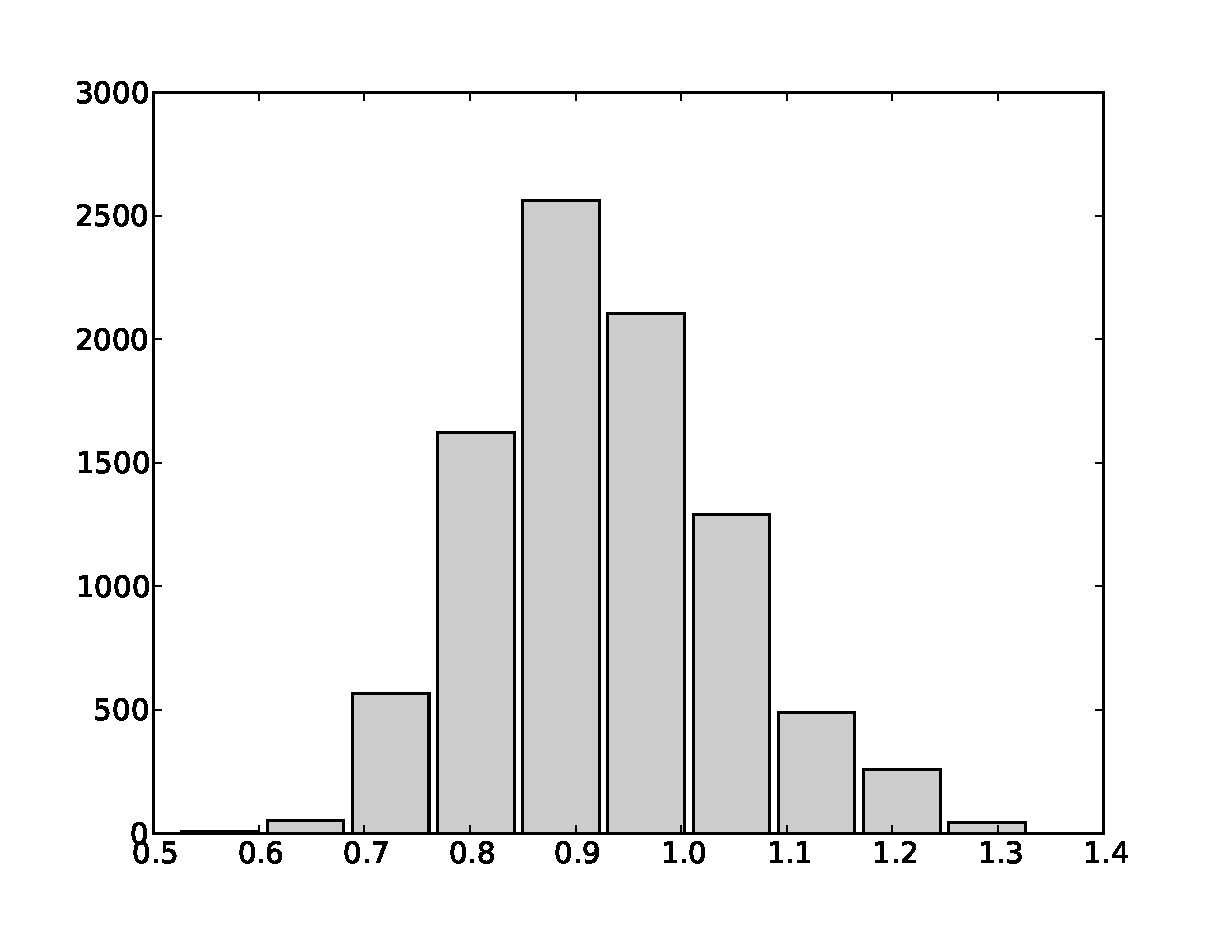
\epsfig{file=ltrace.pdf, width=10cm}
\end{center}
\pkg{PyMC} has its own plotting functionality, via the optional
\code{matplotlib} module as noted in the installation notes. The
\code{Matplot} module includes a \code{plot} function that takes the
model (or a single parameter) as an argument:
\begin{CodeInput}
\begin{CodeChunk}
   >>> from pymc.Matplot import plot
   >>> plot(M)
\end{CodeChunk}
\end{CodeInput}
For each variable in the model, \code{plot} generates a composite figure, such as this one for the switchpoint in the disasters model:
\begin{center}
   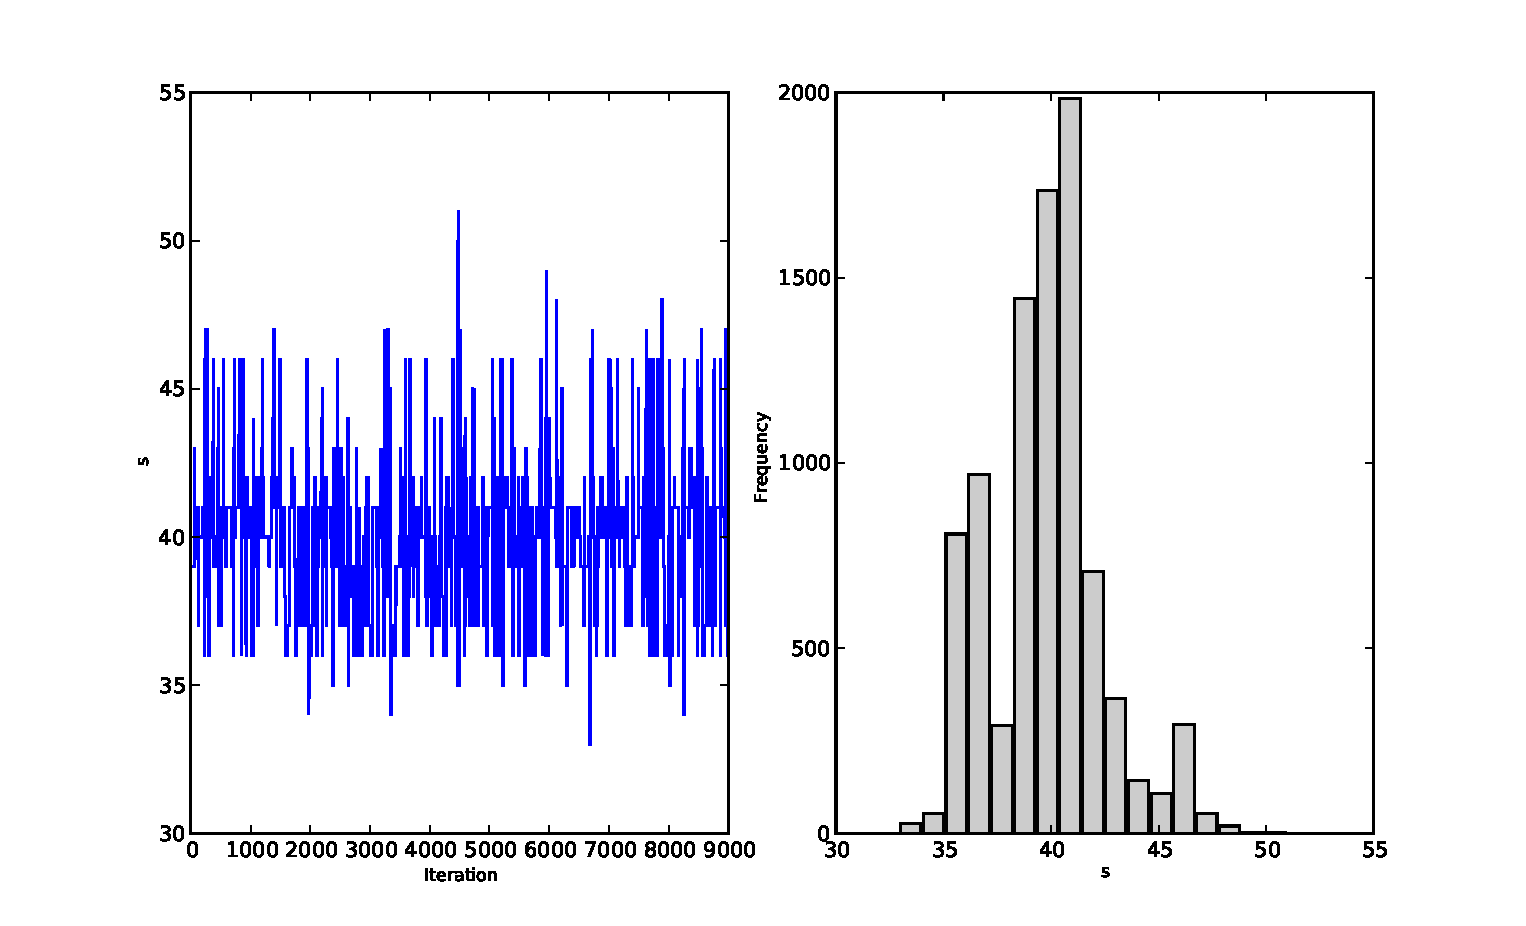
\epsfig{file=spost.pdf, width=15cm}
\end{center}
The left-hand pane of this figure shows the temporal series of the samples from $s$, while the right-hand pane shows a histogram of the trace. The trace is useful for evaluating and diagnosing the algorithm's performance (see \cite*{gelman}), while the histogram is useful for visualizing the posterior.

For a non-graphical summary of the posterior, simply call \code{M.stats()}.

\hypertarget{missing}{}
\subsubsection\*{Imputation of Missing Data} % (fold)

%\label{subsec:missing_data}

As with most ``textbook examples", the models we have examined so far assume that the associated data are complete. That is, there are no missing values corresponding to any observations in the dataset. However, many real-world datasets contain one or more missing values, usually due to some logistical problem during the data collection process. The easiest way of dealing with observations that contain missing values is simply to exclude them from the analysis. However, this results in loss of information if an excluded observation contains valid values for other quantities, and can bias results. An alternative is to impute the missing values, based on information in the rest of the model.

For example, consider a survey dataset for some wildlife species:

\begin{center}
\begin{tabular}{cccc}
\hline
Count & Site & Observer & Temperature\\
\hline
15 & 1 & 1 & 15\\
10 & 1 & 2 & NA\\
6 & 1 & 1 & 11\\
\hline
\end{tabular}
\end{center}

Each row contains the number of individuals seen during the survey, along with three covariates: the site on which the survey was conducted, the observer that collected the data, and the temperature during the survey. If we are interested in modelling, say, population size as a function of the count and the associated covariates, it is difficult to accommodate the second observation because the temperature is missing (perhaps the thermometer was broken that day). Ignoring this observation will allow us to fit the model, but it wastes information that is contained in the other covariates.

In a Bayesian modelling framework, missing data are accommodated simply by treating them as unknown model parameters. Values for the missing data $\tilde{y}$ are estimated naturally, using the posterior predictive distribution:

\begin{equation}
	p(\tilde{y}|y) = \int p(\tilde{y}|\theta) f(\theta|y) d\theta
\end{equation}

This describes additional data $\tilde{y}$, which may either be considered unobserved data or potential future observations. We can use the posterior predictive distribution to model the likely values of missing data.

Consider the coal mining disasters data introduced previously. Assume that two years of data are missing from the time series; we indicate this in the data array by the use of an arbitrary placeholder value, None.

\begin{CodeInput}
\begin{CodeChunk}
x = numpy.array([ 4, 5, 4, 0, 1, 4, 3, 4, 0, 6, 3, 3, 4, 0, 2, 6,
3, 3, 5, 4, 5, 3, 1, 4, 4, 1, 5, 5, 3, 4, 2, 5,
2, 2, 3, 4, 2, 1, 3, None, 2, 1, 1, 1, 1, 3, 0, 0,
1, 0, 1, 1, 0, 0, 3, 1, 0, 3, 2, 2, 0, 1, 1, 1,
0, 1, 0, 1, 0, 0, 0, 2, 1, 0, 0, 0, 1, 1, 0, 2,
3, 3, 1, None, 2, 1, 1, 1, 1, 2, 4, 2, 0, 0, 1, 4,
0, 0, 0, 1, 0, 0, 0, 0, 0, 1, 0, 0, 1, 0, 1])
\end{CodeChunk}
\end{CodeInput}

To estimate these values in \pkg{PyMC}, we generate a masked array. These are specialised \pkg{NumPy} arrays that contain a matching True or False value for each element to indicate if that value should be excluded from any computation. Masked arrays can be generated using \pkg{NumPy}'s \code{ma.masked_equal} function:
\begin{CodeInput}
\begin{CodeChunk}
>>> masked_data = numpy.ma.masked_equal(x, value=None)
>>> masked_data
masked_array(data = [4 5 4 0 1 4 3 4 0 6 3 3 4 0 2 6 3 3 5 4 5 3 1 4 4 1 5 5 3
 4 2 5 2 2 3 4 2 1 3 -- 2 1 1 1 1 3 0 0 1 0 1 1 0 0 3 1 0 3 2 2 0 1 1 1 0 1 0
 1 0 0 0 2 1 0 0 0 1 1 0 2 3 3 1 -- 2 1 1 1 1 2 4 2 0 0 1 4 0 0 0 1 0 0 0 0 0 1
 0 0 1 0 1],
 mask = [False False False False False False False False False False False False
 False False False False False False False False False False False False
 False False False False False False False False False False False False
 False False False  True False False False False False False False False
 False False False False False False False False False False False False
 False False False False False False False False False False False False
 False False False False False False False False False False False  True
 False False False False False False False False False False False False
 False False False False False False False False False False False False
 False False False],
      fill_value=?)

\end{CodeChunk}
\end{CodeInput}

This masked array, in turn, can then be passed to \pkg{PyMC}'s own \code{Impute} function, which replaces the missing values with Stochastic variables of the desired type. For the coal mining disasters problem, recall that disaster events were modelled as Poisson variates:

\begin{CodeInput}
\begin{CodeChunk}
	>>> from pymc import Impute
	>>> D = Impute('D', Poisson, masked_data, mu=r)
	>>> D
	[<pymc.distributions.Poisson 'D[0]' at 0x4ba42d0>,
	 <pymc.distributions.Poisson 'D[1]' at 0x4ba4330>,
	 <pymc.distributions.Poisson 'D[2]' at 0x4ba44d0>,
	 <pymc.distributions.Poisson 'D[3]' at 0x4ba45f0>,
	...
	 <pymc.distributions.Poisson 'D[110]' at 0x4ba46d0>]
\end{CodeChunk}
\end{CodeInput}

Here $r$ is an array of means for each year of data, allocated according to the location of the switchpoint. Each element in $D$ is a Poisson Stochastic, irrespective of whether the observation was missing or not. The difference is that actual observations are data Stochastics (\code{observed=True}), while the missing values are non-data Stochastics. The latter are considered unknown, rather than fixed, and therefore estimated by the MCMC algorithm, just as unknown model parameters.

In this example, we have manually generated the masked array for illustration. In practice, the \code{Impute} function will mask arrays automatically, replacing all \code{None} values with Stochastics. Hence, only the original data array needs to be passed.

The entire model looks very similar to the original model:

\begin{CodeInput}
\begin{CodeChunk}
	# Switchpoint
	s = DiscreteUniform('s', lower=0, upper=110)
	# Early mean
	e = Exponential('e', beta=1)
	# Late mean
	l = Exponential('l', beta=1)

	@deterministic(plot=False)
	def r(s=s, e=e, l=l):
	    """Allocate appropriate mean to time series"""
	    out = numpy.empty(len(disasters_array))
	    # Early mean prior to switchpoint
	    out[:s] = e
	    # Late mean following switchpoint
	    out[s:] = l
	    return out

	# Where the value of x is None, the value is taken as missing.
	D = Impute('D', Poisson, x, mu=r)
\end{CodeChunk}
\end{CodeInput}

\begin{figure}[ht]
\begin{center}
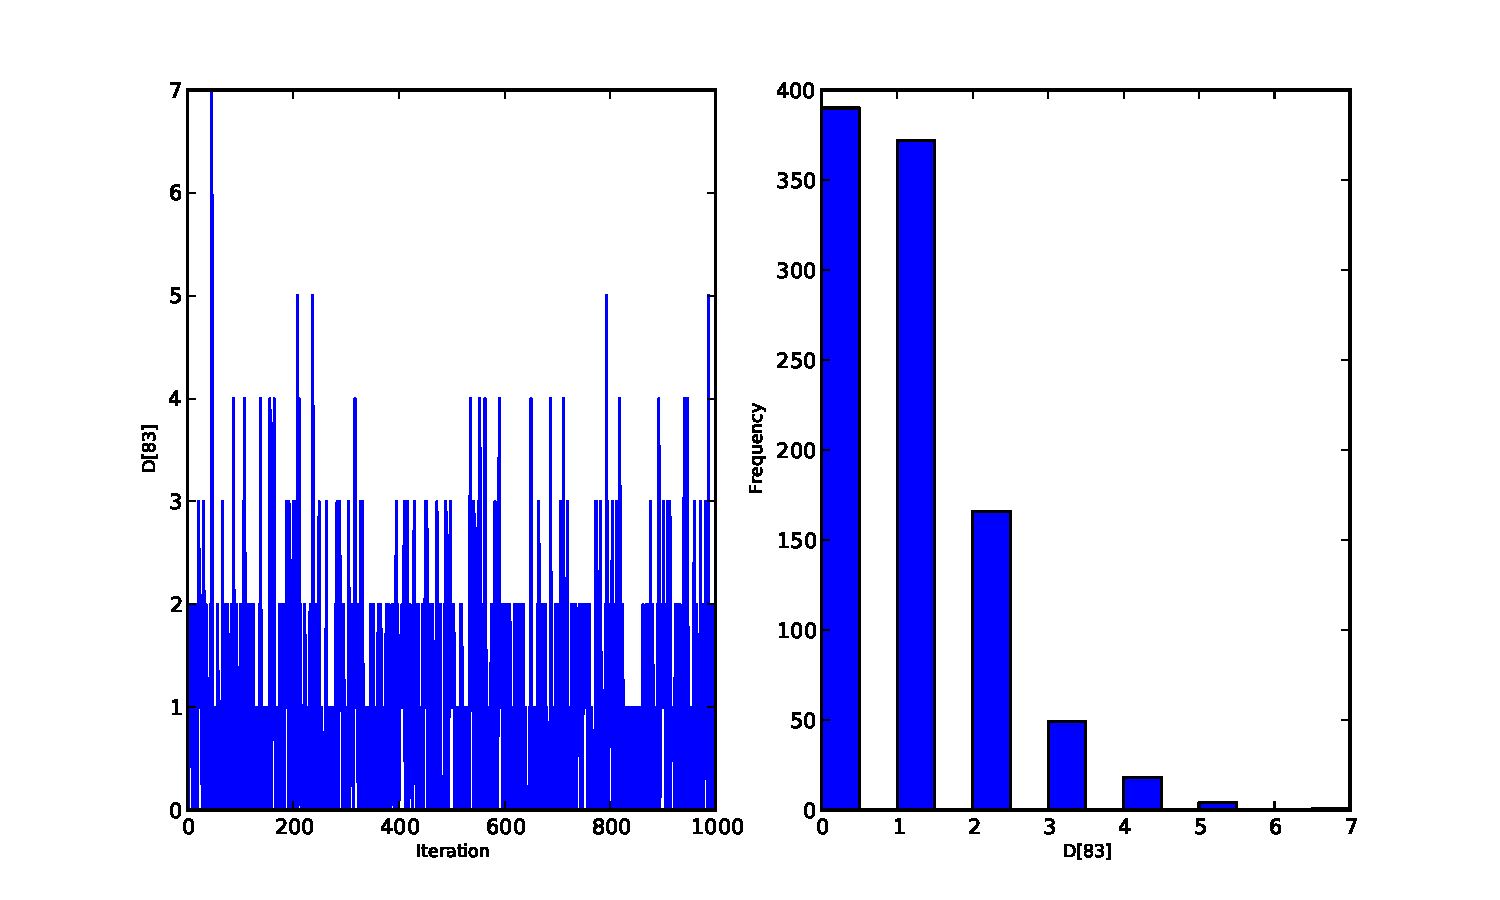
\includegraphics[height=3in]{missing.pdf}
\caption{Trace and posterior distribution of the second missing data point in the example.}
\label{fig:missing}
\end{center}
\end{figure}


The main limitation of this approach for imputation is performance. Because each
element in the data array is modelled by an individual Stochastic, rather than a
single Stochastic for the entire array, the number of nodes in the overall model
increases from 4 to 113. This significantly slows the rate of sampling, due to
the overhead costs associated with iterations over individual nodes.

% Section~missing_data (end)


\subsection{Fine-tuning the MCMC algorithm}

MCMC objects handle individual variables via \emph{step methods}, which determine how parameters are updated at each step of the MCMC algorithm. By default, step methods are automatically assigned to variables by \pkg{PyMC}. To see which step methods $M$ is using, look at its \code{step_method_dict} attribute with respect to each parameter:
\begin{CodeInput}
\begin{CodeChunk}
   >>> M.step_method_dict[DisasterModel.s]
   [<pymc.StepMethods.DiscreteMetropolis object at 0x3e8cb50>]

   >>> M.step_method_dict[DisasterModel.e]
   [<pymc.StepMethods.Metropolis object at 0x3e8cbb0>]

   >>> M.step_method_dict[DisasterModel.l]
   [<pymc.StepMethods.Metropolis object at 0x3e8ccb0>]
\end{CodeChunk}
\end{CodeInput}
The value of \code{step_method_dict} corresponding to a particular variable is a list of the step methods $M$ is using to handle that variable.

You can force $M$ to use a particular step method by calling \code{M.use_step_method} before telling it to sample. The following call will cause $M$ to handle $l$ with a standard \code{Metropolis} step method, but with proposal standard deviation equal to $2$:
\begin{CodeInput}
\begin{CodeChunk}
   >>> from pymc import Metropolis
   M.use_step_method(Metropolis, DisasterModel.l, proposal_sd=2.)
\end{CodeChunk}
\end{CodeInput}

Another step method class, \code{AdaptiveMetropolis}, is better at handling highly-correlated variables. If your model mixes poorly, using \code{AdaptiveMetropolis} is a sensible first thing to try.



\subsection{Beyond the basics}
That was a brief introduction to basic \pkg{PyMC} usage. Many more topics are covered in the subsequent sections, including:
\begin{itemize}
   \item Class \code{Potential}, another building block for probability models in addition to \code{Stochastic} and \code{Deterministic}
   \item Normal approximations
   \item Using custom probability distributions
   \item Object architecture
   \item Saving traces to the disk, or streaming them to the disk during sampling
   \item Writing your own step methods and fitting algorithms.
\end{itemize}
Also, be sure to check out the documentation for the Gaussian process extension,
which is available on \pkg{PyMC}'s
\href{http://code.google.com/p/pymc/downloads/list}{download} page.



\section[Building Models]{Building models}
\label{chap:modelbuilding}
%!TEX root = guide2.0.tex

% \subsection{Summary}\label{sec:\pkg{PyMC}Objects}
Bayesian inference begins with specification of a probability model relating unknown variables to data. \pkg{PyMC} provides three basic building blocks for probability models: \code{Stochastic}, \code{Deterministic} and \code{Potential}.

A \code{Stochastic} object represents a variable whose value is not completely determined by its parents, and a \code{Deterministic} object represents a variable that is entirely determined by its parents. \code{Stochastic} and \code{Deterministic} are subclasses of the \code{Variable} class, which only serves as a template for other classes and is never actually implemented in models.

The third basic class, \code{Potential}, represents `factor potentials' (\cite{dawidmarkov,Jordan:2004p5439}), which are \emph{not} variables but simply terms and/or constraints that are multiplied into joint distributions to modify them. \code{Potential} and \code{Variable} are subclasses of \code{Node}.

% TODO: Need a better description of what a Potential is. Given the description of Stochastic and Deterministic we have given, its not clear where Potential fits in, as it classifies the world into 2 things -- completely determined by parents and not.

% \pkg{PyMC} also provides container classes for variables to make it easier to program of certain dependency situations, such as when a variable is defined by its dependence on an entire Markov chain.

\medskip
\pkg{PyMC} probability models are simply linked groups of \code{Stochastic}, \code{Deterministic} and \code{Potential} objects. These objects have very limited awareness of the models in which they are embedded and do not themselves possess methods for updating their values in fitting algorithms. Objects responsible for fitting probability models are described in Section~\ref{chap:modelfitting}.



\subsection[The Stochastic class]{The \code{Stochastic} class}
\label{stochastic}


A stochastic variable has the following primary attributes:
\begin{description}
    \item[\code{value}:] The variable's current value.
    \item[\code{logp}:] The log-probability of the variable's current value given the values of its parents.
\end{description}
A stochastic variable can optionally be endowed with a method called \code{\bfseries rand}, which draws a value for the variable given the values of its parents\footnote{Note that the \code{random} method does not provide a Gibbs sample unless the variable has no children.}. Stochastic variables have the following additional attributes:
\begin{description}
    \item[\code{parents}:] A dictionary containing the variable's parents. The keys of the dictionary are to the labels assigned to the parents by the variable, and the values correspond to the actual parents. For example, the keys of $s$'s parents dictionary in model (\ref{disastermodel}) would be \code{'t_l'} and \code{'t_h'}. The actual parents (\emph{i.e.} the values of the dictionary) may be of any class or type.
    \item[\code{children}:] A set containing the variable's children.
    \item[\code{extended_parents}:] A set containing all the stochastic variables on which the variable depends either directly or via a sequence of deterministic variables. If the value of any of these variables changes, the variable will need to recompute its log-probability.
    \item[\code{extended_children}:] A set containing all the stochastic variables and potentials that depend on the variable either directly or via a sequence of deterministic variables. If the variable's value changes, all of these variables and potentials will need to recompute their log-probabilities.
    % \item[\code{coparents}:] A set containing all the stochastic variables that share extended children with the variable.
    % \item[\code{moral_neighbors}:] A set containing the union of the variable's extended parents, extended children and coparents, with Potential objects removed.
    % \item[\code{markov_blanket}:] A set containing self and self's moral neighbors.
    \item[\code{observed}:] A flag (boolean) indicating whether the variable's value has been observed (is fixed).
    \item[\code{dtype}:] A \pkg{NumPy} dtype object (such as \code{numpy.int}) that specifies the type of the variable's value. The variable's value is always cast to this type. If this is \code{None} (default) then no type is enforced.
    % \item[\code{__name__}:] The name of the variable, should be unique.
    %    \item[\code{__doc__}:] The docstring of the variable.
\end{description}

\subsubsection\*{Creation of stochastic variables}
There are three main ways to create stochastic variables, called the \textbf{automatic}, \textbf{decorator}, and \textbf{direct} interfaces.

\begin{description}
    \item[Automatic] Stochastic variables with standard distributions provided by \pkg{PyMC} (see Section~\ref{chap:distributions}) can be created in a single line using special subclasses of \code{Stochastic}. For example, the uniformly-distributed discrete variable $s$ in (\ref{disastermodel}) could be created using the automatic interface as follows:
\begin{CodeInput}
\begin{CodeChunk}
    import pymc as pm
    s = pm.DiscreteUniform('s', 1851, 1962, value=1900)
\end{CodeChunk}
\end{CodeInput}

    In addition to the classes in Section~\ref{chap:distributions}, \code{scipy.stats.distributions}' random variable classes are wrapped as \code{Stochastic} subclasses if \pkg{SciPy} is installed. These distributions are in the submodule \code{pymc.\pkg{SciPy}Distributions}.

    Users can call the class factory \code{stochastic_from_dist} to produce \code{Stochastic} subclasses of their own from probability distributions not included with \pkg{PyMC}.%  These classes' init methods take the following arguments:
    % \begin{description}
    %     \item[\code{name}:] The name of the variable.
    %     \item[\code{value}:] An initial value for the variable.
    %     \item[\code{parents}:] Keyword arguments specifying the parents of the variable.
    %     \item[\code{observed} (optional)]
    %     \item[\code{doc} (optional):] The docstring of the variable.
    %     \item[\code{verbose} (optional):] An integer from 0 to 3.
    %     \item[\code{trace} (optional):] A boolean indicating whether a trace should be kept for this variable in Monte Carlo fitting methods.
    %     \item[\code{cache_depth}:] See Section~\ref{sec:caching}.
    % \end{description}


    \item[Decorator] Uniformly-distributed discrete stochastic variable $s$ in (\ref{disastermodel}) could alternatively be created from a function that computes its log-probability as follows:
\begin{CodeInput}
\begin{CodeChunk}
@pm.stochastic(dtype=int)
def s(value=1900, t_l=1851, t_h=1962):
    """The switchpoint for the rate of disaster occurrence."""
    if value > t_h or value < t_l:
        # Invalid values
        return -numpy.inf
    else:
        # Uniform log-likelihood
        return -numpy.log(t_h - t_l + 1)
\end{CodeChunk}
\end{CodeInput}
Note that this is a simple \proglang{Python} function preceded by a \proglang{Python} expression called a \href{http://docs.python.org/glossary.html#term-decorator}{decorator}, here called \code{@stochastic}. Generally, decorators enhance functions with additional properties or functionality. The \code{Stochastic} object produced by the \code{@stochastic} decorator will evaluate its log-probability using the function $s$. The \code{value} argument, which is required, provides an initial value for the variable. The remaining arguments will be assigned as parents of $s$ (\emph{i.e.} they will populate the \code{parents} dictionary).

To emphasize, the \proglang{Python} function decorated by \code{@stochastic} should compute the \emph{log}-density or \emph{log}-probability of the variable. That's why the return value in the example above is $-\log(t_h-t_l+1)$ rather than $1/(t_h-t_l+1)$.

The \code{value} and parents of stochastic variables may be any objects, provided the log-probability function returns a real number (\code{float}). \pkg{PyMC} and \pkg{SciPy} both provide implementations of several standard probability distributions that may be helpful for creating custom stochastic variables. Based on informal comparison using version 2.0, the distributions in \pkg{PyMC} tend to be approximately an order of magnitude faster than their counterparts in \pkg{SciPy} (using version 0.7). See \href{http://code.google.com/p/pymc/wiki/Benchmarks}{the wiki page on benchmarks}.

    The decorator \code{stochastic} can take any of the arguments \code{Stochastic.__init__} takes except \code{parents}, \code{logp}, \code{random}, \code{doc} and \code{value}. These arguments include \code{trace}, \code{plot}, \code{verbose}, \code{dtype}, \code{rseed} and \code{name}.

    The decorator interface has a slightly more complex implementation which allows you to specify a \code{random} method for sampling the stochastic variable's value conditional on its parents.
    \begin{CodeInput}
\begin{CodeChunk}
@pm.stochastic(dtype=int)
def s(value=1900, t_l=1851, t_h=1962):
    """The switchpoint for the rate of disaster occurrence."""

    def logp(value, t_l, t_h):
        if value > t_h or value < t_l:
            return -numpy.inf
        else:
            return -numpy.log(t_h - t_l + 1)

    def random(t_l, t_h):
        return numpy.round( (t_l - t_h) * random() ) + t_l

    \end{CodeChunk}
\end{CodeInput}
The stochastic variable again gets its name, docstring and parents from function $s$, but in this case it will evaluate its log-probability using the \code{logp} function. The \code{random} function will be used when \code{s.random()} is called. Note that \code{random} doesn't take a \code{value} argument, as it generates values itself.

    \item[Direct] It's possible to instantiate \code{Stochastic} directly:
\begin{CodeInput}
\begin{CodeChunk}
def s_logp(value, t_l, t_h):
    if value > t_h or value < t_l:
        return -numpy.inf
    else:
        return -numpy.log(t_h - t_l + 1)

def s_rand(t_l, t_h):
    return numpy.round( (t_l - t_h) * random() ) + t_l

s = pm.Stochastic( logp = s_logp,
                doc = 'The switchpoint for the rate of disaster occurrence.',
                name = 's',
                parents = {'t_l': 1851, 't_h': 1962},
                random = s_rand,
                trace = True,
                value = 1900,
                dtype=int,
                rseed = 1.,
                observed = False,
                cache_depth = 2,
                plot=True,
                verbose = 0)
\end{CodeChunk}
\end{CodeInput}
Notice that the log-probability and random variate functions are specified externally and passed to \code{Stochastic} as arguments. This is a rather awkward way to instantiate a stochastic variable; consequently, such implementations should be rare.

\end{description}

\begin{center}
\begin{boxedminipage}{.9\textwidth}
\subsubsection\*{Don't update stochastic variables' values in-place}


\code{Stochastic} objects' values should not be updated in-place. This confuses \pkg{PyMC}'s caching scheme and corrupts the process used for accepting or rejecting proposed values in the MCMC algorithm. The only way a stochastic variable's value should be updated is using statements of the following form:
\begin{CodeInput}
\begin{CodeChunk}
    A.value = new_value
\end{CodeChunk}
\end{CodeInput}
The following are in-place updates and should \emph{never} be used:
\begin{itemize}
    \item \code{A.value += 3}
    \item \code{A.value[2,1] = 5}
    \item \code{A.value.attribute = new_attribute_value}.
\end{itemize}

This restriction becomes onerous if a step method proposes values for the elements of an array-valued variable separately. In this case, it may be preferable to partition the variable into several scalar-valued variables stored in an array or list.
\end{boxedminipage}
\end{center}


\subsection{Data} \label{data}


Data are represented by \code{Stochastic} objects whose \code{observed} attribute is set to \code{True}. Although the data are modelled with statistical distributions, their values should be treated as immutable (since they have been observed). If a stochastic variable's \code{observed} flag is \code{True}, its value cannot be changed, and it won't be sampled by the fitting method.

\subsubsection\*{Declaring stochastic variables to be data}

In each interface, an optional keyword argument \code{observed} can be set to \code{True}. In the decorator interface, this argument is added to the \code{@stochastic} decorator:

\begin{CodeInput}
\begin{CodeChunk}
@pm.stochastic(observed=True)
\end{CodeChunk}
\end{CodeInput}

In the other interfaces, the \code{observed=True} argument is added to the initialization arguments:

\begin{CodeInput}
\begin{CodeChunk}
	x = pm.Binomial('x', value=7, n=10, p=.8, observed=True)
\end{CodeChunk}
\end{CodeInput}

Alternatively, in the decorator interface only, a \code{Stochastic} object's \code{observed} flag can be set to true by stacking an \code{@observed} decorator on top of the \code{@stochastic} decorator:
\begin{CodeInput}
\begin{CodeChunk}
@observed
@stochastic(dtype=int)
\end{CodeChunk}
\end{CodeInput}


\subsection[The Deterministic class]{The \code{Deterministic} class}
\label{deterministic}


The \code{Deterministic} class represents variables whose values are completely determined by the values of their parents. For example, in model (\ref{disastermodel}), $r$ is a \code{deterministic} variable. Recall it was defined by
\begin{eqnarray*}
    r_t=\left\{\begin{array}{ll}
        e & t\le s\\ l & t>s
        \end{array}\right.,
\end{eqnarray*}
so $r$'s value can be computed exactly from the values of its parents $e$, $l$ and $s$.

A \code{deterministic} variable's most important attribute is \code{\bfseries value}, which gives the current value of the variable given the values of its parents. Like \code{Stochastic}'s \code{logp} attribute, this attribute is computed on-demand and cached for efficiency.

A Deterministic variable has the following additional attributes:
\begin{description}
    \item[\code{parents}:] A dictionary containing the variable's parents. The keys of the dictionary correspond to the labels assigned to the parents, and the values correspond to the actual parents.
    \item[\code{children}:] A set containing the variable's children, which must be nodes (variables or potentials).
    % \item[\code{__name__}:] The name of the variable, should be unique.
    %     \item[\code{__doc__}:] The docstring of the variable.
\end{description}
Deterministic variables have no methods.


\subsubsection\*{Creation of deterministic variables}
There are several ways to create deterministic variables:
\begin{description}
   \item[Automatic] A handful of common functions have been wrapped in Deterministic subclasses. These are brief enough to list:
   \begin{description}
      \item[\code{LinearCombination}:] Has two parents $x$ and $y$, both of which must be iterable (\emph{i.e.} vector-valued). The value of a linear combination is
      \[
      \sum_i x_i^T y_i.
      \]
      \item[\code{Index}:] Has two parents $x$ and \code{index}. $x$ must be iterable, \code{index} must be valued as an integer. The value of an index is
      \[
      x[\mathtt{index}].
      \]
      \code{Index} is useful for implementing dynamic models, in which the parent-child connections change.
      \item[\code{Lambda}:] Converts an anonymous function (in \proglang{Python}, called \textbf{lambda functions}) to a \code{Deterministic} instance on a single line.
      \item[\code{CompletedDirichlet}:] \pkg{PyMC} represents Dirichlet variables of length $k$ by the first $k-1$ elements; since they must sum to 1, the $k-$th element is determined by the others. \code{CompletedDirichlet} appends the $k-$th element to the value of its parent $D$.
      \item[\code{Logit}, \code{InvLogit}, \code{StukelLogit}, \code{StukelInvLogit}:] Two common link functions for generalized linear models and their inverses.
   \end{description}
   It's a good idea to use these classes when feasible in order to give hints to step methods.

   \item[Elementary operations on variables] Certain elementary operations on variables create deterministic variables. For example:   
\begin{CodeInput}
\begin{CodeChunk}
>>> x = pm.MvNormalCov('x',numpy.ones(3),numpy.eye(3))
>>> y = pm.MvNormalCov('y',numpy.ones(3),numpy.eye(3))
>>>
>>> print x+y
<pymc.\pkg{PyMC}Objects.Deterministic '(x_add_y)' at 0x105c3bd10>
>>>
>>> print x[0]
<pymc.CommonDeterministics.Index 'x[0]' at 0x105c52390>
>>>
>>> print x[1]+y[2]
<pymc.\pkg{PyMC}Objects.Deterministic '(x[1]_add_y[2])' at 0x105c52410>
\end{CodeChunk}
\end{CodeInput}

All the objects thus created have \code{trace=False} and \code{plot=False} by default. This convenient method of generating simple deterministics was inspired by \cite{fbc}.

    \item[Decorator] A deterministic variable can be created via a decorator in a way very similar to \code{Stochastic}'s decorator interface:
\begin{CodeInput}
\begin{CodeChunk}
@pm.deterministic
def r(switchpoint = s, early_rate = e, late_rate = l):
    """The rate of disaster occurrence."""
    value = numpy.zeros(len(D))
    value[:switchpoint] = early_rate
    value[switchpoint:] = late_rate
    return value
\end{CodeChunk}
\end{CodeInput}
Notice that rather than returning the log-probability, as is the case for \code{Stochastic} objects, the function returns the value of the deterministic object, given its parents. This return value may be of any type, as is suitable for the problem at hand. Also notice that, unlike for \code{Stochastic} objects, there is no \code{value} argument passed, since the value is calculated deterministically by the function itself. Arguments' keys and values are converted into a parent dictionary as with \code{Stochastic}'s short interface. The \code{deterministic} decorator can take \code{trace}, \code{verbose} and \code{plot} arguments, like the \code{stochastic} decorator\footnote{Note that deterministic variables have no \code{observed} flag. If a deterministic variable's value were known, its parents would be restricted to the inverse image of that value under the deterministic variable's evaluation function. This usage would be extremely difficult to support in general, but it can be implemented for particular applications at the \code{StepMethod} level.}.

    \item[Direct] \code{Deterministic} can also be instantiated directly:
\begin{CodeInput}
\begin{CodeChunk}
def r_eval(switchpoint = s, early_rate = e, late_rate = l):
    value = numpy.zeros(len(D))
    value[:switchpoint] = early_rate
    value[switchpoint:] = late_rate
    return value

r = pm.Deterministic(  eval = r_eval,
                    name = 'r',
                    parents = {'switchpoint': s, 'early_rate': e, 'late_rate': l},
                    doc = 'The rate of disaster occurrence.',
                    trace = True,
                    verbose = 0,
                    dtype=float,
                    plot=False,
                    cache_depth = 2)
\end{CodeChunk}
\end{CodeInput}
\end{description}


\subsection{Containers} \label{container}

In some situations it would be inconvenient to assign a unique label to each parent of a variable. Consider $y$ in the following model:
\begin{align*}
    x_0 &\sim \textup N (0,\tau_x)\\
    x_{i+1}|x_i &\sim \textup{N}(x_i, \tau_x)
    &i=0,\ldots, N-2\\
    y|x &\sim \textup N \left(\sum_{i=0}^{N-1}x_i^2,\tau_y\right)
\end{align*}
Here, $y$ depends on every element of the Markov chain $x$, but we wouldn't want to manually enter $N$ parent labels \code{`x_0'}, \code{`x_1'}, etc.

This situation can be handled naturally in \pkg{PyMC}:
\begin{CodeInput}
\begin{CodeChunk}
N = 10
x_0 = pm.Normal('x_0', mu=0, tau=1)

# Initialize array of stochastics
x = numpy.empty(N,dtype=object)
x[0] = x_0

# Loop over number of elements in N
for i in range(1,N):

   # Create Normal stochastic, whose mean is the previous element in x
   x[i] = pm.Normal('x_%i' % i, mu=x[i-1], tau=1)

@pm.observed
@pm.stochastic
def y(value = 1, mu = x, tau = 100):
    return pm.normal_like(value, numpy.sum(mu**2), tau)
\end{CodeChunk}
\end{CodeInput}
\pkg{PyMC} automatically wraps array $x$ in an appropriate \code{Container} class. The  expression \code{`x_\%i'\%i} labels each \code{Normal} object in the container with the appropriate index $i$; so if \code{i=1}, the name of the corresponding element becomes \code{`x_1'}.

Containers, like variables, have an attribute called \code{value}. This attribute returns a copy of the (possibly nested) iterable that was passed into the container function, but with each variable inside replaced with its corresponding value.

Containers can currently be constructed from lists, tuples, dictionaries, Numpy arrays, modules, sets or any object with a \code{__dict__} attribute. Variables and non-variables can be freely mixed in these containers, and different types of containers can be nested\footnote{Nodes whose parents are containers make private shallow copies of those containers. This is done for technical reasons rather than to protect users from accidental misuse.}. Containers attempt to behave like the objects they wrap. All containers are subclasses of \code{ContainerBase}.

Containers have the following useful attributes in addition to \code{value}:
\begin{itemize}
    \item\code{variables}
    \item\code{stochastics}
    \item\code{potentials}
    \item\code{deterministics}
    \item\code{data_stochastics}
    \item\code{step_methods}.
\end{itemize}
Each of these attributes is a set containing all the objects of each type in a container, and within any containers in the container.



\subsection[The Potential class]{The \code{Potential} class} \label{potential}


% See the two examples here and the extended example below. Is that enough?

The joint density corresponding to model (\ref{disastermodel}) can be written as follows:
\begin{eqnarray*}
    p(D,s,l,e) = p(D|s,l,e) p(s) p(l) p(e).
\end{eqnarray*}
Each factor in the joint distribution is a proper, normalized probability distribution for one of the variables conditional on its parents. Such factors are contributed by \code{Stochastic} objects.

In some cases, it's nice to be able to modify the joint density by incorporating terms that don't correspond to probabilities of variables conditional on parents, for example:
\begin{eqnarray*}
    p(x_0, x_2, \ldots x_{N-1}) \propto \prod_{i=0}^{N-2} \psi_i(x_i, x_{i+1}).
\end{eqnarray*}


In other cases we may want to add probability terms to existing models. For example, suppose we want to constrain the difference between $e$ and $l$ in (\ref{disastermodel}) to be less than 1, so that the joint density becomes
\begin{eqnarray*}
    p(D,s,l,e) \propto p(D|s,l,e) p(s) p(l) p(e) I(|e-l|<1).
\end{eqnarray*}
It's possible to express this constraint by adding variables to the model, or by grouping $e$ and $l$ to form a vector-valued variable, but it's uncomfortable to do so.

Arbitrary factors such as $\psi$ and the indicator function $I(|e-l|<1)$ are
implemented by objects of class \code{Potential} (\cite{dawidmarkov} and
\cite{Jordan:2004p5439} call these terms `factor potentials'). Bayesian
hierarchical notation (cf model (\ref{disastermodel})) doesn't accomodate these
potentials. They are often used in cases where there is no natural dependence
hierarchy, such as the first example above (which is known as a Markov random
field). They are also useful for expressing `soft data'
\citep{Christakos:2002p5506} as in the second example above.


\bigskip
Potentials have one important attribute, \code{\bfseries logp}, the log of their current probability or probability density value given the values of their parents. The only other attribute of interest is \code{parents}, a dictionary containing the potential's parents. Potentials have no methods. They have no \code{trace} attribute, because they are not variables. They cannot serve as parents of variables (for the same reason), so they have no \code{children} attribute.google map

\subsubsection\*{An example of soft data}
The role of potentials can be confusing, so we will provide another example: we have a dataset $t$ consisting of the days on which several marked animals were recaptured. We believe that the probability $S$ that an animal is not recaptured on any given day can be explained by a covariate vector $x$. We model this situation as follows:
\begin{eqnarray*}
    t_i|S_i \sim \textup{Geometric}(S_i), & i=1\ldots N\\
    S_i = \textup{logit}^{-1}(\beta x_i), &i=1\ldots N\\
    \beta\sim \textup{N}(\mu_\beta, V_\beta).
\end{eqnarray*}
So far, so good. Now suppose we have some knowledge of other related experiments and we have a good idea of what $S$ will be independent of the value of $\beta$. It's not obvious how to work this `soft data', because as we've written the model $S$ is completely determined by $\beta$. There are three options within the strict Bayesian hierarchical framework:
\begin{itemize}
    \item Work the soft data into the prior on $\beta$.
    \item Incorporate the data from the previous experiments explicitly into the model.
    \item Refactor the model so that $S$ is at the bottom of the hierarchy, and assign the prior directly.
\end{itemize}

Factor potentials provide a convenient way to incorporate the soft data without the need for such major modifications. We can simply modify the joint distribution from
\begin{eqnarray*}
    p(t|S(x,\beta)) p(\beta)
\end{eqnarray*}
to
\begin{eqnarray*}
    \gamma(S) p(t|S(x,\beta)) p(\beta),
\end{eqnarray*}
where the value of $\gamma$ is large if $S$'s value is plausible (based on our external information) and small otherwise. We do not know the normalizing constant for the new distribution, but we don't need it to use most popular fitting algorithms. It's a good idea to check the induced priors on $S$ and $\beta$ for sanity. This can be done in \pkg{PyMC} by fitting the model with the data $t$ removed.

It's important to understand that $\gamma$ is not a variable, so it does not have a value. That means, among other things, there will be no $\gamma$ column in MCMC traces.


\subsubsection\*[Creation of Potentials]{Creation of \code{Potentials}}
There are two ways to create potentials:
\begin{description}
    \item[Decorator] A potential can be created via a decorator in a way very similar to \code{Deterministic}'s decorator interface:
\begin{CodeInput}
\begin{CodeChunk}
@pm.potential
def psi_i(x_lo = x[i], x_hi = x[i+1]):
    """A pair potential"""
    return -(x_lo - x_hi)**2
\end{CodeChunk}
\end{CodeInput}
The function supplied should return the potential's current \emph{log}-probability or \emph{log}-density as a Numpy \code{float}. The \code{potential} decorator can take \code{verbose} and \code{cache_depth} arguments like the \code{stochastic} decorator.
    \item[Direct] The same potential could be created directly as follows:
\begin{CodeInput}
\begin{CodeChunk}
def psi_i_logp(x_lo = x[i], x_hi = x[i+1]):
    return -(x_lo - x_hi)**2

psi_i = pm.Potential(  logp = psi_i_logp,
                    name = 'psi_i',
                    parents = {'xlo': x[i], 'xhi': x[i+1]},
                    doc = 'A pair potential',
                    verbose = 0,
                    cache_depth = 2)
\end{CodeChunk}
\end{CodeInput}
\end{description}



\subsection{Graphing models} \label{graphical}


The function \code{graph} in \code{pymc.graph} draws graphical representations of \code{Model} (Section~\ref{chap:modelfitting}) instances using GraphViz via the \proglang{Python} package PyDot. See \cite{dawidmarkov} and \cite{Jordan:2004p5439} for more discussion of useful information that can be read off of graphical models. Note that these authors do not consider deterministic variables.

The symbol for stochastic variables is an ellipse. Parent-child relationships are indicated by arrows. These arrows point from parent to child and are labeled with the names assigned to the parents by the children. \pkg{PyMC}'s symbol for deterministic variables is a downward-pointing triangle. A graphical representation of model \ref{disastermodel} follows:
\begin{center}
    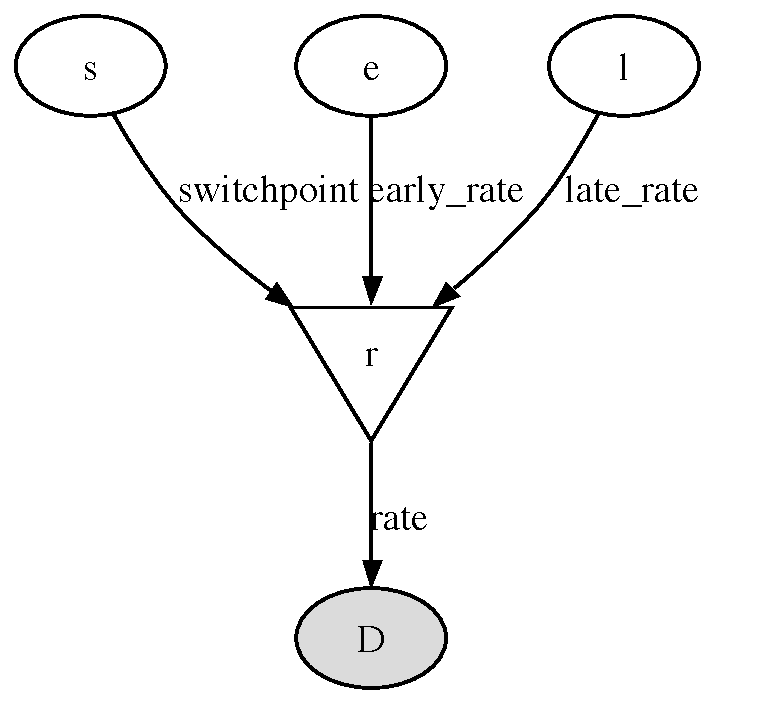
\epsfig{file=DisasterModel2.pdf, width=6cm}
\end{center}
$D$ is shaded because it is flagged as data.

% Note that if a deterministic variable has more than one child, its parents each inherit all of its children when it is made implicit:
% \begin{center}
%     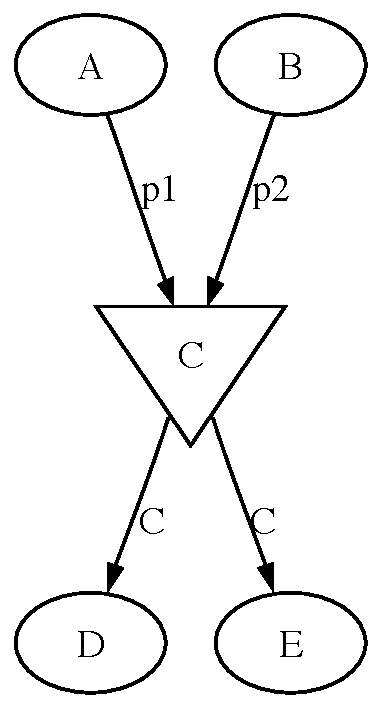
\epsfig{file=DeterministicPreInheritance.pdf, width=3.5cm} $\Rightarrow$ 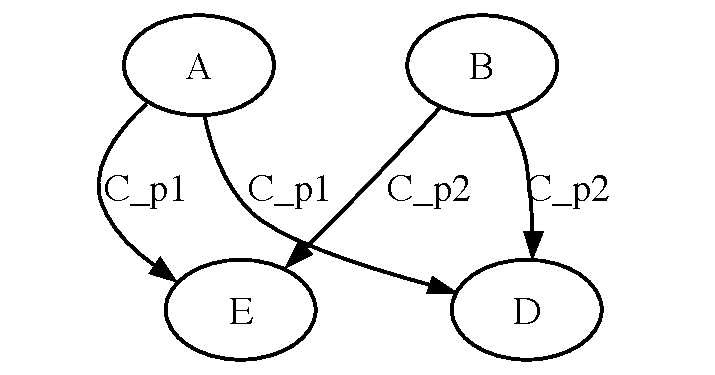
\epsfig{file=DeterministicPostInheritance.pdf, width=5cm}
% \end{center}
% These inherited children can be accessed via the \code{extended_children} attributes of the parents.

The symbol for factor potentials is a rectangle, as in the following model.
\begin{center}
    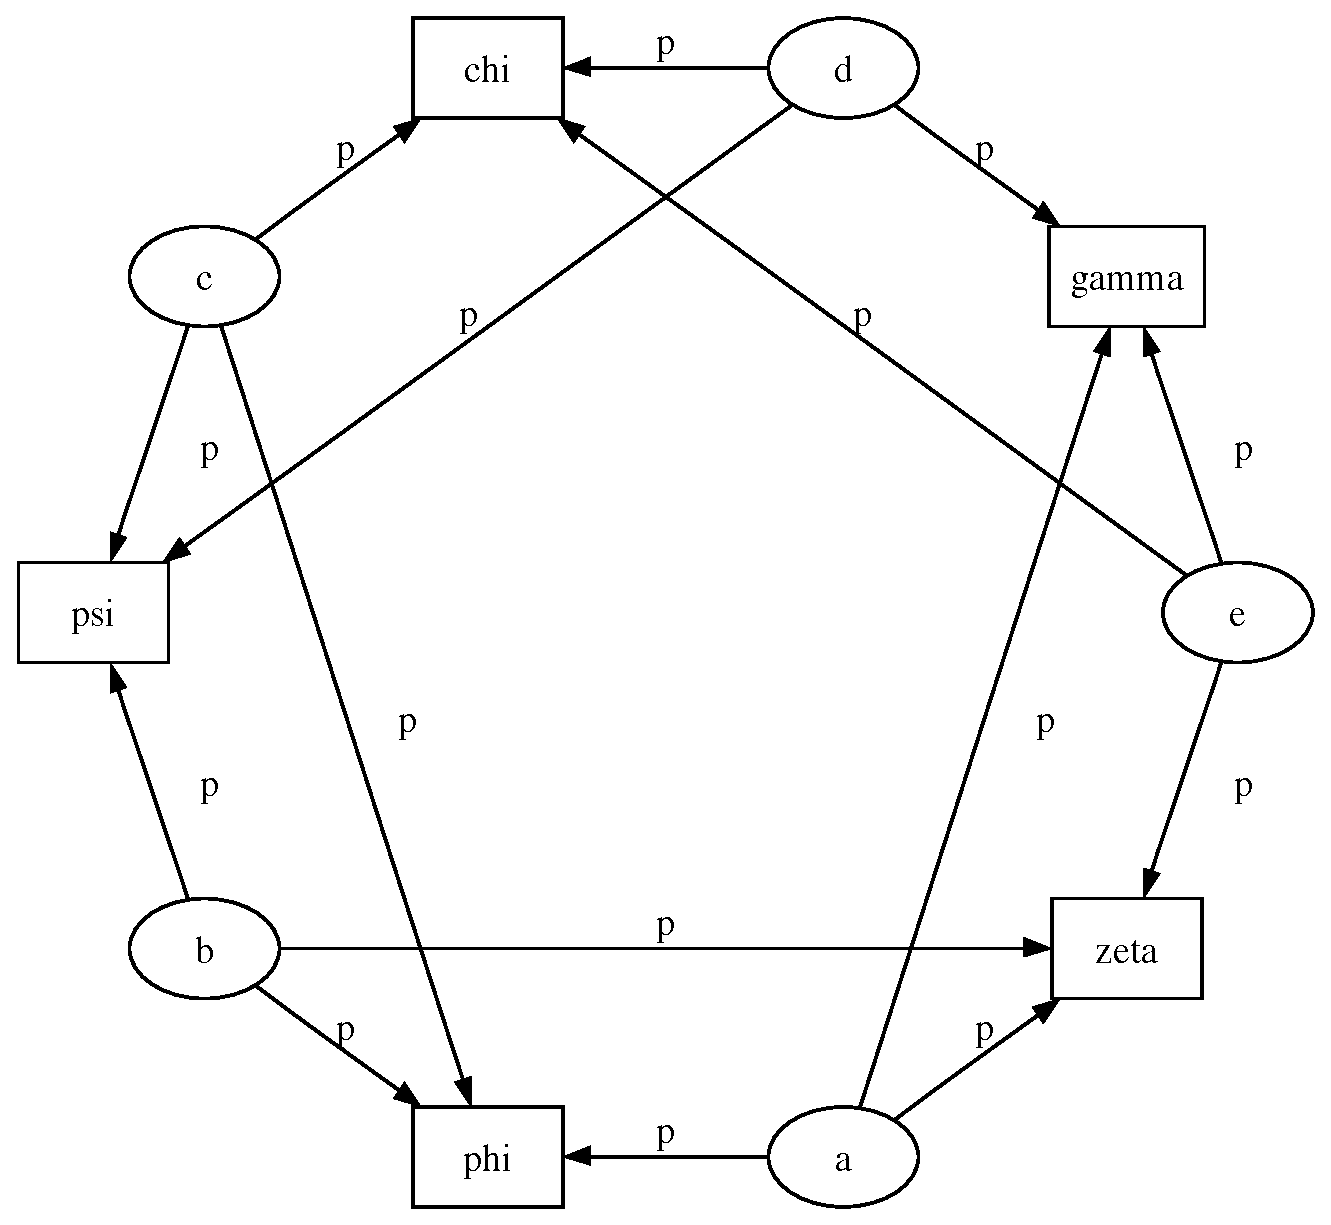
\epsfig{file=PotExample.pdf, width=10cm}
\end{center}
Factor potentials are usually associated with \emph{undirected} grahical models. In undirected representations, each parent of a potential is connected to every other parent by an undirected edge. The undirected representation of the model pictured above is much more compact:
\begin{center}
    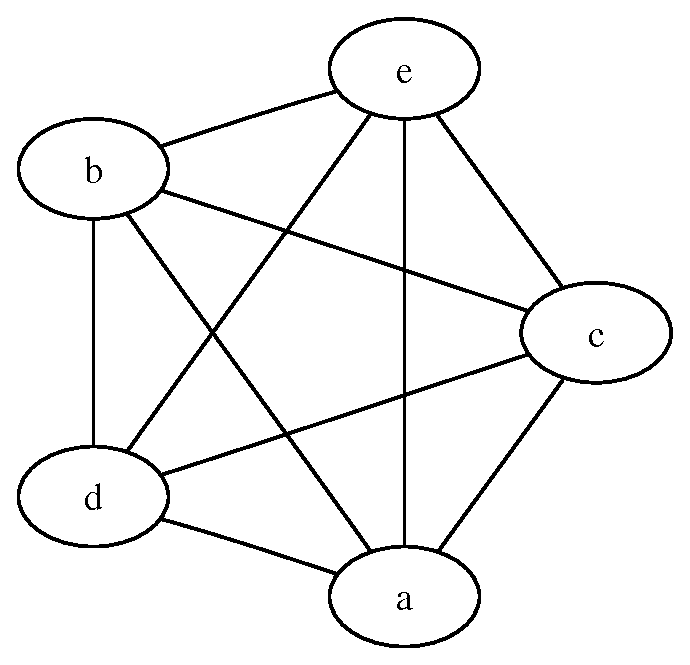
\epsfig{file=PotExampleCollapsed.pdf, width=5cm}
\end{center}
Directed or mixed graphical models can be represented in an undirected form by `moralizing', which is done by the function \code{pymc.graph.moral_graph}.


\subsection[Class LazyFunction and caching]{Class \code{LazyFunction}
and caching}
\label{sec:caching}
This Section~gives an overview of how \pkg{PyMC} computes log-probabilities. This is advanced information that is not required in order to use \pkg{PyMC}.

The \code{logp} attributes of stochastic variables and potentials and the \code{value} attributes of deterministic variables are wrappers for instances of class \code{LazyFunction}. Lazy functions are wrappers for ordinary \proglang{Python} functions. A lazy function \code{L} could be created from a function \code{fun} as follows:
\begin{CodeInput}
\begin{CodeChunk}
L = pm.LazyFunction(fun, arguments)
\end{CodeChunk}
\end{CodeInput}
The argument \code{arguments} is a dictionary container; \code{fun} must accept keyword arguments only. When \code{L}'s \code{get()} method is called, the return value is the same as the call
\begin{CodeInput}
\begin{CodeChunk}
fun(**arguments.value)
\end{CodeChunk}
\end{CodeInput}
Note that no arguments need to be passed to \code{L.get}; lazy functions memorize their arguments.

Before calling \code{fun}, \code{L} will check the values of its arguments' extended children against an internal cache. This comparison is done \emph{by reference}, not by value, and this is part of the reason why stochastic variables' values cannot be updated in-place. If the arguments' extended children's values match a frame of the cache, the corresponding output value is returned and \code{fun} is not called. If a call to \code{fun} is needed, the arguments' extended children's values and the return value replace the oldest frame in the cache. The depth of the cache can be set using the optional init argument \code{cache_depth}, which defaults to 2.

Caching is helpful in MCMC, because variables' log-probabilities and values tend to be queried multiple times for the same parental value configuration. The default cache depth of 2 turns out to be most useful in Metropolis-Hastings-type algorithms involving proposed values that may be rejected.

Lazy functions are implemented in C using \href{http://www.cosc.canterbury.ac.nz/greg.ewing/python/\pkg{Pyrex}/}{\pkg{Pyrex}} , a language for writing \proglang{Python} extensions.



\section[Fitting Models]{Fitting models}
\label{chap:modelfitting}
% \pkg{PyMC} probability models are linked collections of nodes. These nodes are only informed by the values of their parents. \code{Deterministic} instances can compute their values given their parents' values, \code{Stochastic} instances can compute their log-probabilities or draw new values, and \code{Potential} instances can compute their log-probabilities. Fitting probability models requires larger-scale coordination and communication.

\pkg{PyMC} provides three objects that fit models:
\begin{itemize}
    \item \code{MCMC}, which coordinates Markov chain Monte Carlo algorithms. The actual work of updating stochastic variables conditional on the rest of the model is done by \code{StepMethod} objects, which are described in this section.
    \item \code{MAP}, which computes maximum \emph{a posteriori} estimates.
    \item \code{NormApprox}, which computes the `normal approximation' \citep{gelman}: the joint distribution of all stochastic variables in a model is approximated as normal using local information at the maximum \emph{a posteriori} estimate.
\end{itemize}

All three objects are subclasses of \code{Model}, which is \pkg{PyMC}'s base class for fitting methods. \code{MCMC} and \code{NormApprox}, both of which can produce samples from the posterior, are subclasses of \code{Sampler}, which is \pkg{PyMC}'s base class for Monte Carlo fitting methods. \code{Sampler} provides a generic sampling loop method and database support for storing large sets of joint samples. These base classes are documented at the end of this section. %Sampling loops can optionally be run interactively, meaning the user can pause sampling at any time, return to the \proglang{Python} prompt, check progress, and make adjustments.

\subsection{Creating models} \label{sec:ModelInstantiation}
The first argument to any fitting method's \code{init} method, including that of \code{MCMC}, is called \code{input}. The \code{input} argument can be just about anything; once you have defined the nodes that make up your model, you shouldn't even have to think about how to wrap them in a \code{Model} instance. Some examples of model instantiation using nodes \code{a}, \code{b} and \code{c} follow:
\begin{itemize}
    \item \code{M = Model(set([a,b,c]))}
    \item \code{M = Model(\{`a': a, `d': [b,c]\})} In this case, $M$ will expose $a$ and $d$ as attributes: \code{M.a} will be $a$, and \code{M.d} will be \code{[b,c]}.
    \item \code{M = Model([[a,b],c])}
    \item If file \code{MyModule} contains the definitions of \code{a}, \code{b} and \code{c}:
   \begin{CodeInput}
\begin{CodeChunk}
import MyModule
M = Model(MyModule)
    \end{CodeChunk}
\end{CodeInput}
    In this case, $M$ will expose $a$, $b$ and $c$ as attributes.
    \item Using a `model factory' function:
    \begin{CodeInput}
\begin{CodeChunk}
def make_model(x):
    a = pm.Exponential('a',beta=x,value=0.5)

    @pm.deterministic
    def b(a=a):
        return 100-a

    @pm.stochastic
    def c(value=0.5, a=a, b=b):
        return (value-a)**2/b

    return locals()

M = pm.Model(make_model(3))
    \end{CodeChunk}
\end{CodeInput}
    In this case, $M$ will also expose $a$, $b$ and $c$ as attributes.
\end{itemize}

\subsubsection\*[The Model class]{The \code{Model} class} \label{sec:Model}
\code{Model} serves as a container for probability models and as a base class for the classes responsible for model fitting, such as \code{MCMC}.

\code{Model}'s init method takes the following arguments:
\begin{description}
    \item[\code{input}:] Some collection of \pkg{PyMC} nodes defining a probability model. These may be stored in a list, set, tuple, dictionary, array, module, or any object with a \code{__dict__} attribute.
    \item[\code{verbose} (optional):] An integer controlling the verbosity of the model's output.
\end{description}

Models' useful methods are:
\begin{description}
    \item[\code{draw_from_prior()}:] Sets all stochastic variables' values to new random values, which would be a sample from the joint distribution if all data and \code{Potential} instances' log-probability functions returned zero. If any stochastic variables lack a \code{random()} method, \pkg{PyMC} will raise an exception.
    \item[\code{seed()}:] Same as \code{draw_from_prior}, but only \code{stochastics} whose \code{rseed} attribute is not \code{None} are changed.
\end{description}

The helper function \code{graph} produces graphical representations of models \cite[see]{Jordan:2004p5439}.

Models have the following important attributes:
\begin{itemize}
    \item \code{variables}
    \item \code{stochastics}
    \item \code{potentials}
    \item \code{deterministics}
    \item \code{observed_stochastics}
    \item \code{step_methods}
    \item \code{value}: A copy of the model, with each attribute that is a \pkg{PyMC} variable or container replaced by its value.
    \item \code{generations}: A \href{http://en.wikipedia.org/wiki/Topological_sort}{topological sorting} of the stochastics in the model.
\end{itemize}

In addition, models expose each node they contain as an attribute. For instance, if model \code{M} were produced from model (\ref{disastermodel}) \code{M.s} would return the switchpoint variable.


\subsection{Maximum \emph{a posteriori} estimates} \label{sec:MAP}

The \code{MAP} class sets all stochastic variables to their maximum \emph{a posteriori} values using functions in \pkg{SciPy}'s \code{optimize} package. \pkg{SciPy} must be installed to use it. \code{MAP} can only handle variables whose dtype is \code{float}, so it will not work on model \ref{disastermodel}. To fit the model in \code{examples/gelman_bioassay.py} using \code{MAP}, do the following
\begin{CodeInput}
\begin{CodeChunk}
>>> from pymc.examples import gelman_bioassay
>>> M = pm.MAP(gelman_bioassay)
>>> M.fit()
\end{CodeChunk}
\end{CodeInput}
This call will cause $M$ to fit the model using Nelder-Mead optimization, which does not require derivatives. The variables in \code{gelman_bioassay} have now been set to their maximum \emph{a posteriori} values:
\begin{CodeInput}
\begin{CodeChunk}
>>> M.alpha.value
array(0.8465892309923545)
>>> M.beta.value
array(7.7488499785334168)
\end{CodeChunk}
\end{CodeInput}
In addition, the AIC and BIC of the model are now available:
\begin{CodeInput}
\begin{CodeChunk}
>>> M.AIC
7.9648372671389458
>>> M.BIC
6.7374259893787265
\end{CodeChunk}
\end{CodeInput}

\bigskip
\code{MAP} has two useful methods:
\begin{description}
    \item[\code{fit(method ='fmin', iterlim=1000, tol=.0001)}:] The optimization method may be \code{fmin}, \code{fmin_l_bfgs_b}, \code{fmin_ncg}, \code{fmin_cg}, or \code{fmin_powell}. See the documentation of \pkg{SciPy}'s \code{optimize} package for the details of these methods. The \code{tol} and \code{iterlim} parameters are passed to the optimization function under the appropriate names.
    \item[\code{revert_to_max()}:] If the values of the constituent stochastic variables change after fitting, this function will reset them to their maximum \emph{a posteriori} values.
\end{description}
If you're going to use an optimization method that requires derivatives, \code{MAP}'s \code{init} method can take additional parameters \code{eps} and \code{diff_order}. \code{diff_order}, which must be an integer, specifies the order of the numerical approximation (see the \pkg{SciPy} function \code{derivative}). The step size for numerical derivatives is controlled by \code{eps}, which may be either a single value or a dictionary of values whose keys are variables (actual objects, not names).

The useful attributes of \code{MAP} are:
\begin{description}
    \item[\code{logp}:] The joint log-probability of the model.
    \item[\code{logp_at_max}:] The maximum joint log-probability of the model.
    % \item[\code{len}:] The total number of elements in all the stochastic variables in the model with \code{observed=False}.
    % \item[\code{data_len}:] The total number number of elements in all the stochastic variables in the model with \code{observed=True}.
    \item[\code{AIC}:] Akaike's information criterion for this model \citep{Akaike:1973aj,Burnham:2002ic}.
    \item[\code{BIC}:] The Bayesian information criterion for this model \citep{Schwarz:1978ud}.
\end{description}

One use of the \code{MAP} class is finding reasonable initial states for MCMC chains. Note that multiple \code{Model} subclasses can handle the same collection of nodes.

\subsection{Normal approximations} \label{sec:norm-approx}

The \code{NormApprox} class extends the \code{MAP} class by approximating the posterior covariance of the model using the Fisher information matrix, or the Hessian of the joint log probability at the maximum. To fit the model in \code{examples/gelman_bioassay.py} using \code{NormApprox}, do:
\begin{CodeInput}
\begin{CodeChunk}
>>> N = pm.NormApprox(gelman_bioassay)
>>> N.fit()
\end{CodeChunk}
\end{CodeInput}
The approximate joint posterior mean and covariance of the variables are available via the attributes \code{mu} and \code{C}:
\begin{CodeInput}
\begin{CodeChunk}
>>> N.mu[N.alpha]
array([ 0.84658923])
>>> N.mu[N.alpha, N.beta]
array([ 0.84658923,  7.74884998])
>>> N.C[N.alpha]
matrix([[ 1.03854093]])
>>> N.C[N.alpha, N.beta]
matrix([[  1.03854093,   3.54601911],
        [  3.54601911,  23.74406919]])
\end{CodeChunk}
\end{CodeInput}
As with \code{MAP}, the variables have been set to their maximum \emph{a posteriori} values (which are also in the \code{mu} attribute) and the AIC and BIC of the model are available.

In addition, it's now possible to generate samples from the posterior as with \code{MCMC}:
\begin{CodeInput}
\begin{CodeChunk}
>>> N.sample(100)
>>> N.trace('alpha')[::10]
array([-0.85001278,  1.58982854,  1.0388088 ,  0.07626688,  1.15359581,
       -0.25211939,  1.39264616,  0.22551586,  2.69729987,  1.21722872])
>>> N.trace('beta')[::10]
array([  2.50203663,  14.73815047,  11.32166303,   0.43115426,
        10.1182532 ,   7.4063525 ,  11.58584317,   8.99331152,
        11.04720439,   9.5084239 ])
\end{CodeChunk}
\end{CodeInput}
Any of the database backends can be used (Section~\ref{chap:database}).

\bigskip
In addition to the methods and attributes of \code{MAP}, \code{NormApprox} provides the following methods:
\begin{description}
    \item[\code{sample(iter)}:] Samples from the approximate posterior distribution are drawn and stored.
    \item[\code{isample(iter)}:] An `interactive' version of \code{sample()}: sampling can be paused, returning control to the user.
    \item[\code{draw}:] Sets all variables to random values drawn from the approximate posterior.
\end{description}
It provides the following additional attributes:
\begin{description}
    \item[\code{mu}:] A special dictionary-like object that can be keyed with multiple variables. \code{N.mu[p1, p2, p3]} would return the approximate posterior mean values of stochastic variables \code{p1}, \code{p2} and \code{p3}, ravelled and concatenated to form a vector.
    \item[\code{C}:] Another special dictionary-like object. \code{N.C[p1, p2, p3]} would return the approximate posterior covariance matrix of stochastic variables \code{p1}, \code{p2} and \code{p3}. As with \code{mu}, these variables' values are ravelled and concatenated before their covariance matrix is constructed.
\end{description}

\subsection[Markov chain Monte Carlo: the MCMC class]{Markov chain Monte
Carlo: the \code{MCMC} class} \label{sec:mcmc}

The \code{MCMC} class implements \pkg{PyMC}'s core business: producing `traces' for a model's variables which can be considered sequences of joint samples from the posterior. See Section~\ref{chap:tutorial} for an example of basic usage.

\code{MCMC}'s primary job is to create and coordinate a collection of `step methods', each of which is responsible for updating one or more variables. The available step methods are described below. Instructions on how to create your own step method are available in Section~\ref{chap:extending}.

\code{MCMC} provides the following useful methods:
\begin{description}
    \item[\code{sample(iter, burn, thin, tune\_interval, tune\_throughout, save\_interval, verbose)}:] Runs the MCMC algorithm and produces the traces. The \code{iter} argument controls the total number of MCMC iterations. No tallying will be done during the first \code{burn} iterations; these samples will be forgotten. After this burn-in period, tallying will be done each \code{thin} iterations. Tuning will be done each \code{tune\_interval} iterations. If \code{tune\_throughout=False}, no more tuning will be done after the burnin period. The model state will be saved every \code{save\_interval} iterations, if given.
    \item[\code{isample(iter, burn, thin, tune\_interval, tune\_throughout, save\_interval, verbose)}:] An interactive version of \code{sample}. The sampling loop may be paused at any time, returning control to the user.
    \item[\code{use_step_method(method, *args, **kwargs)}:] Creates an instance of step method class \code{method} to handle some stochastic variables. The extra arguments are passed to the \code{init} method of \code{method}. Assigning a step method to a variable manually will prevent the \code{MCMC} instance from automatically assigning one. However, you may handle a variable with multiple step methods.
    % \item[\code{assign_step_methods()}:] Assigns step methods to all stochastic variables that do not currently have any. This method is called whenever \code{sample} or \code{isample} is called, but it can be useful to call it directly to see what the default step methods will be.

    % A variable is assigned a step method as follows: each eligible \code{StepMethod} subclass in existence is allowed to inspect the variable in question and determine its competence to handle the variable, on a scale of 0 to 3. An instance of the highest bidder is created to handle the variable.
    \item[\code{goodness()}:] Calculates goodness-of-fit (GOF) statistics according to \cite{Brooks:2000il}.
    \item[\code{save\_state()}:] Saves the current state of the sampler, including all stochastics, to the database. This allows the sampler to be reconstituted at a later time to resume sampling. This is not supported yet for the RDBMS backends, sqlite and mysql.
    \item[\code{restore\_state()}:] Restores the sampler to the state stored in the database.
	 \item[\code{stats()}:] Generates summary statistics for all nodes in the model.
    \item[\code{remember(trace\_index)}:] Set all variables' values from frame \code{trace\_index} in the database.
\end{description}

MCMC samplers' step methods can be accessed via the \code{\textbf{step_method_dict}} attribute. \code{M.step_method_dict[x]} returns a list of the step methods \code{M} will use to handle the stochastic variable \code{x}.

After sampling, the information tallied by \code{M}  can be queried via \code{M.db.trace_names}. In addition to the values of variables, tuning information for adaptive step methods is generally tallied. These `traces' can be plotted to verify that tuning has in fact terminated.

You can produce `traces' for arbitrary functions with zero arguments as well. If you issue the command \code{M._funs_to_tally['trace_name'] = f} before sampling begins, then each time the model variables' values are tallied \code{f} will be called with no arguments, and the return value will be tallied. After sampling ends you can retrieve the trace as \code{M.trace['trace_name']}

\subsubsection\*[The Sampler class]{The \code{Sampler} class} \label{sec:Sampler}
\code{MCMC} is a subclass of a more general class called \code{Sampler}. Samplers fit models with Monte Carlo fitting methods, which characterize the posterior distribution by approximate samples from it. They are initialized as follows: \code{Sampler(input=None, db='ram', name='Sampler', reinit_model=True, calc_deviance=False)}. The \code{input} argument is a module, list, tuple, dictionary, set, or object that contains all elements of the model, the \code{db} argument indicates which database backend should be used to store the samples (see Section~\ref{chap:database}), \code{reinit\_model} is a boolean flag that indicates whether the model should be re-initialised before running, and \code{calc\_deviance} is a boolean flag indicating whether deviance should be calculated for the model at each iteration. Samplers have the following important methods:
\begin{description}
    \item[\code{sample(iter, length=None, verbose=0)}:] Samples from the joint distribution. The \code{iter} argument controls how many times the sampling loop will be run, and the \code{length} argument controls the initial size of the database that will be used to store the samples.
    \item[\code{isample(iter, length=None, verbose=0)}:] The same as \code{sample}, but the sampling is done interactively: you can pause sampling at any point and be returned to the \proglang{Python} prompt to inspect progress and adjust fitting parameters. While sampling is paused, the following methods are useful:
    \begin{description}
        \item[\code{icontinue()}:] Continue interactive sampling.
        \item[\code{halt()}:] Truncate the database and clean up.
    \end{description}
    \item[\code{tally()}:] Write all variables' current values to the database. The actual write operation depends on the specified database backend.
    %\item[\code{draw()}:] Not currently used. In future Monte Carlo fitting methods that aren't MCMC, such as importance samplers, the \code{draw()} method will be responsible for drawing approximate samples from the joint distribution (by setting the values of all the stochastic variables in the model).
    \item[\code{save\_state()}:] Saves the current state of the sampler, including all stochastics, to the database. This allows the sampler to be reconstituted at a later time to resume sampling. This is not supported yet for the RDBMS backends, sqlite and mysql.
    \item[\code{restore\_state()}:] Restores the sampler to the state stored in the database.
	 \item[\code{stats()}:] Generates summary statistics for all nodes in the model.
    \item[\code{remember(trace\_index)}:] Set all variables' values from frame \code{trace\_index} in the database. Note that the \code{trace_index} is different from the current iteration, since not all samples are necessarily saved due to burning and thinning.
\end{description}

In addition, the sampler attribute \code{deviance} is a deterministic variable valued as the model's deviance at its current state.


\subsection{Step methods} \label{sec:stepmethod}


Step method objects handle individual stochastic variables, or sometimes groups of them. They are responsible for making the variables they handle take single MCMC steps conditional on the rest of the model. Each subclass of \code{StepMethod} implements a method called \code{step()}, which is called by \code{MCMC}. Step methods with adaptive tuning parameters can optionally implement a method called \code{tune()}, which causes them to assess performance so far and adjust.

The major subclasses of \code{StepMethod} are \code{Metropolis},
\code{AdaptiveMetropolis} and \code{Gibbs}. \pkg{PyMC} provides several flavors of the
basic Metropolis steps, but the Gibbs steps are not ready for use as of the
current release. However, because it is feasible to write Gibbs step methods
for particular applications, the \code{Gibbs} base class will be documented
here.

\subsubsection\*{Metropolis step methods} \label{metropolis}

\code{Metropolis} and subclasses implement Metropolis-Hastings steps. To tell an \code{MCMC} object $M$ to handle a variable $x$ with a Metropolis step method, you might do the following:
\begin{CodeInput}
\begin{CodeChunk}
M.use_step_method(pm.Metropolis, x, proposal_sd=1., proposal_distribution='Normal')
\end{CodeChunk}
\end{CodeInput}

\code{Metropolis} itself handles float-valued variables, and subclasses \code{DiscreteMetropolis} and \code{BinaryMetropolis} handle integer- and boolean-valued variables, respectively. Subclasses of \code{Metropolis} must implement the following methods:
\begin{description}
    \item[\code{propose()}:] Sets the values of the variables handled by the Metropolis step method to proposed values.
    \item[\code{reject()}:] If the Metropolis-Hastings acceptance test fails, this method is called to reset the values of the variables to their values before \code{propose()} was called.
\end{description}
Note that there is no \code{accept()} method; if a proposal is accepted, the variables' values are simply left alone. Subclasses that use proposal distributions other than symmetric random-walk may specify the `Hastings factor' by changing the \code{hastings\_factor} method. See Section~\ref{chap:extending} for an example.

\code{Metropolis}' \code{init} method takes the following arguments:
\begin{description}
   \item[\code{stochastic}:] The variable to handle.
   \item[\code{proposal_sd}:] A float or array of floats. This sets the
    default proposal standard deviation if the proposal distribution is normal.
   \item[\code{scale}:] A float, defaulting to 1. If the \code{scale} argument is provided but not \code{proposal_sd}, \code{proposal\_sd} is computed as follows:
   \begin{CodeInput}
\begin{CodeChunk}
   if all(self.stochastic.value != 0.):
       self.proposal_sd = ones(shape(self.stochastic.value)) * \
                           abs(self.stochastic.value) * scale
   else:
       self.proposal_sd = ones(shape(self.stochastic.value)) * scale
   \end{CodeChunk}
\end{CodeInput}
   \item[\code{proposal_distribution}:] A string indicating which distribution should be used for proposals. Current options are \code{'Normal'} and \code{'Prior'}. If \code{proposal_distribution=None}, the proposal distribution is chosen automatically. It is set to \code{'Prior'} if the variable has no children and has a random method, and to \code{'Normal'} otherwise.
   \item[\code{verbose}:] An integer. By convention, $0$ indicates minimal output and $2$ indicates maximum verbosity.
\end{description}

Although the \code{proposal\_sd} attribute is fixed at creation, Metropolis step methods adjust this initial value using an attribute called \code{adaptive_scale_factor}. When \code{tune()} is called, the acceptance ratio of the step method is examined and this scale factor is updated accordingly. If the proposal distribution is normal, proposals will have standard deviation \code{self.proposal\_sd * self.adaptive_scale_factor}.

By default, tuning will continue throughout the sampling loop, even after the burnin period is over. This can be changed via the \code{tune\_throughout} argument to \code{MCMC.sample}. If an adaptive step method's \code{tally} flag is set (the default for \code{Metropolis}), a trace of its tuning parameters will be kept. If you allow tuning to continue throughout the sampling loop, it is important to verify that the `Diminishing Tuning' condition of \cite{tuning} is satisfied: the amount of tuning should decrease to zero, or tuning should become very infrequent.

If a Metropolis step method handles an array-valued variable, it proposes all elements independently but simultaneously. That is, it decides whether to accept or reject all elements together but it does not attempt to take the posterior correlation between elements into account. The \code{AdaptiveMetropolis} class (see below), on the other hand, does make correlated proposals.

\paragraph\*[The AdaptiveMetropolis class]{The
\code{AdaptiveMetropolis} class}
\label{subsec:AM}
The \code{AdaptativeMetropolis} (AM) step method works like a regular Metropolis
step method, with the exception that its variables are block-updated using a
multivariate jump distribution whose covariance is tuned during sampling.
Although the chain is non-Markovian, it has correct ergodic properties (see
\cite{Haario:2001lr}).

To tell an \code{MCMC} object $M$ to handle variables $x$, $y$ and $z$ with an
\code{AdaptiveMetropolis} instance, you might do the following:
\begin{CodeInput}
\begin{CodeChunk}
   M.use_step_method(pm.AdaptiveMetropolis, [x,y,z], \
                      scales={x:1, y:2, z:.5}, delay=10000)
\end{CodeChunk}
\end{CodeInput}

\code{AdaptativeMetropolis}' init method takes the following arguments:
% cov=None, delay=1000, scales=None, interval=200, greedy=True,verbose=0
\begin{description}
   \item[\code{stochastics}:] The stochastic variables to handle. These will be
updated jointly.
   \item[\code{cov} (optional):] An initial covariance matrix. Defaults to the
identity matrix, adjusted according to the \code{scales} argument.
   \item[\code{delay} (optional):] The number of iterations to delay before
computing the empirical covariance matrix.
   \item[\code{scales} (optional):] The initial covariance matrix will be
diagonal, and its diagonal elements will be set to \code{scales} times the
stochastics' values, squared.
   \item[\code{interval} (optional):] The number of iterations between updates
of the covariance matrix. Defaults to 1000.
   \item[\code{greedy} (optional):] If \code{True}, only accepted jumps will be
counted toward the delay before the covariance is first computed. Defaults to
\code{True}.
   \item[\code{verbose} (optional):] An integer from 0 to 3 controlling the verbosity of
the step method's printed output.
    \item[\code{shrink_if_necessary} (optional):] Whether the proposal covariance should be
shrunk if the acceptance rate becomes extremely small.
\end{description}

In this algorithm, jumps are proposed from a multivariate normal
distribution with covariance matrix $C$. The algorithm first iterates
until \code{delay} samples have been drawn (if \code{greedy} is true, until
\code{delay} jumps have been accepted). At this point, $C$ is given
the value of the empirical covariance of the trace so far and sampling
resumes. The covariance is then updated each \code{interval}
iterations throughout the entire sampling run\footnote{The covariance is
estimated recursively from the previous value and the last \code{interval}
samples, instead of computing it each time from the entire trace.}. It is
this constant adaptation of the proposal distribution that makes the chain
non-Markovian.

\paragraph\*[The DiscreteMetropolis class]{The
\code{DiscreteMetropolis} class}
This class is just like \code{Metropolis}, but specialized to handle
\code{Stochastic} instances with dtype \code{int}. The jump proposal
distribution can either be \code{'Normal'}, \code{'Prior'} or \code{'Poisson'}.
In the normal case, the proposed value is drawn from a normal distribution
centered at the current value and then rounded to the
nearest integer. In the Poisson case, the proposed value is obtained by adding
or substracting (with equal probability) a random value drawn from a Poisson
distribution.

\paragraph\*[The BinaryMetropolis class]{The
\code{BinaryMetropolis} class}
This class is specialized to handle \code{Stochastic} instances with dtype
\code{bool}.

For array-valued variables, \code{BinaryMetropolis} can be set to propose from
the prior by passing in \code{dist="Prior"}. Otherwise, the argument
\code{p_jump} of the init method specifies how probable a change is. Like
\code{Metropolis}' attribute \code{proposal_sd}, \code{p_jump} is tuned
throughout the sampling loop via \code{adaptive_scale_factor}.

For scalar-valued variables, \code{BinaryMetropolis} behaves like a Gibbs
sampler, since this requires no additional expense. The \code{p_jump} and
\code{adaptive_scale_factor} parameters are not used in this case.

% ==========================================================
% = We can uncomment this when we actually release them... =
% ==========================================================
% \hypertarget{gibbs}{}
% \subsubsection\*{Gibbs step methods} \label{gibbs}
% 
%
% Conjugate submodels (see \cite{gelman}) can be handled by Gibbs step methods rather than the default Metropolis methods. Gibbs step methods are Metropolis methods whose acceptance rate is always 1. They can be convenient because they relieve the user from having to worry about tuning the acceptance rate, but they can be computationally expensive. When variables are highly dependent on one another, better mixing can often be obtained by using \code{AdaptiveMetropolis} even when Gibbs step methods are available.
%
% Alpha versions of Gibbs step methods handling the following conjugate submodels are available in the \code{sandbox} module, but they are not recommended and will not be assigned automatically:
% \begin{itemize}
%     \item Gamma-Gamma
%     \item Gamma-Exponential
%     \item Gamma-Poisson
%     \item Gamma-Normal
%     \item Beta-Geometric
%     \item Beta-Binomial
%     \item Wishart-Multivariate Normal (represented by the \code{MvNormal} class, which is parameterized by precision)
%     \item Dirichlet-Multinomial.
%     \item Normal-Normal (or Normal-MvNormal, etc.) (requires \code{cvxopt}, \href{http://abel.ee.ucla.edu/cvxopt}{http://abel.ee.ucla.edu/cvxopt} )
% \end{itemize}
% However, if you implement a custom Gibbs step method, subclassing the \code{Gibbs} class will ensure interopera
%
% Gibbs step methods have the following class attributes:
% \begin{itemize}
%     \item \code{child_class}: The step method can handle variables whose children are all of this class. \code{GammaNormal.child_class} is \code{Normal}, for example.
%     \item \code{parent_label}: The target variable's children must refer to it by this label. \code{GammaNormal.parent_label} is \code{'mu'}.
%     \item \code{target_class}: The target variable should be of this class for the submodel to be fully conjugate. \code{GammaNormal.target_class} is \code{Gamma}.
%     \item \code{linear_OK}: A flag indicating whether the variable's children can depend on a multiple of the variable. Such multiples must be implemented via the \code{Deterministic} subclass \code{LinearCombination}.
% \end{itemize}
%
% A Gibbs step method can handle variables that are not of their target class, as long as all their children are of the appropriate class. If this is the case, the step method's \code{conjugate} attribute will be set to \code{False} and its acceptance rate will no longer be 1.
%
% Gibbs step methods are easy to use manually. To tell an \code{MCMC}
% object $M$ to handle a variable $x$ using the \code{GammaNormal} class,
% simply use the call
% \begin{CodeInput}
\begin{CodeChunk}
%     M.use_step_method(GammaNormal, x)
% \end{CodeChunk}
\end{CodeInput}
%
% To indicate a general preference for Gibbs step methods vs. Metropolis step methods, set the following global integer values:
% \begin{itemize}
%     \item \code{pymc.conjugate_Gibbs_competence}: Applicable Gibbs step methods' competence functions will return this value for variables that are not of their target classes. The default value is 0, meaning that these methods will never be assigned automatically. Set this value to 3 to ensure that Gibbs step methods are always be assigned to conjugate submodels, or to 1.5 to set their priorities between those of \code{Metropolis} and \code{AdaptiveMetropolis}.
%     \item \code{pymc.nonconjugate_Gibbs_competence}: Applicable Gibbs step methods' competence functions will return this value for variables that are of their target classes. The default value is 0, meaning that these methods are never assigned automatically.
% \end{itemize}
%

\subsubsection\*{Granularity of step methods: one-at-a-time vs. block updating}
\label{subsec:granularity}
There is currently no way for a stochastic variable to compute individual terms of its log-probability; it is computed all together. This means that updating the elements of a array-valued variable individually would be inefficient, so all existing step methods update array-valued variables together, in a block update.

To update an array-valued variable's elements individually, simply break it up into an array of scalar-valued variables. Instead of this:
\begin{CodeInput}
\begin{CodeChunk}
A = pm.Normal('A', value=numpy.zeros(100), mu=0., tau=1.)
\end{CodeChunk}
\end{CodeInput}
do this:
\begin{CodeInput}
\begin{CodeChunk}
A = [pm.Normal('A_%i'%i, value=0., mu=0., tau=1.) for i in range(100)]
\end{CodeChunk}
\end{CodeInput}
An individual step method will be assigned to each element of \code{A} in the latter case, and the elements will be updated individually. Note that \code{A} can be broken up into larger blocks if desired.

\subsubsection\*{Automatic assignment of step methods}
Every step method subclass (including user-defined ones) that does not require any \code{init} arguments other than the stochastic variable to be handled adds itself to a list called \code{StepMethodRegistry} in the \pkg{PyMC} namespace. If a stochastic variable in an \code{MCMC} object has not been explicitly assigned a step method, each class in \code{StepMethodRegistry} is allowed to examine the variable.

To do so, each step method implements a class method called \code{competence}, whose only argument is a single stochastic variable. These methods return values from 0 to 3; 0 meaning the step method cannot safely handle the variable and 3 meaning it will most likely be the best available step method for variables like this. The \code{MCMC} object assigns the step method that returns the highest competence value to each of its stochastic variables.




\section[Sampling Results]{Saving and managing sampling results}
\label{chap:database}



\section[Model Checking]{Model checking and diagnostics}
\label{chap:modelchecking}

\subsection{Convergence Diagnostics} % (fold)
%\label{sec:convergence_diagnostics}

Valid inferences from sequences of MCMC samples are based on the assumption that samples are derived from the true posterior distribution of interest. Theory guarantees this condition as the number of iterations approaches infinity. It is important, therefore, to determine the minimum number of samples required to ensure a reasonable approximation to the target posterior density. Unfortunately, no universal threshold exists across all problems, so convergence must be assessed independently each time MCMC estimation is performed. The procedures for verifying convergence are collectively known as convergence diagnostics.

One approach to analyzing convergence is analytical, whereby the variance of the sample at different sections of the chain are compared to that of the limiting distribution. These methods use distance metrics to analyze convergence, or place theoretical bounds on the sample variance, and though they are promising, they are generally difficult to use and are not prominent in the MCMC literature. More common is a statistical approach to assessing convergence. Statistical techniques, rather than considering the properties of the theoretical target distribution, only consider the statistical properties of the observed chain. Reliance on the sample alone restricts such convergence criteria to heuristics, and hence, convergence cannot be guaranteed. Although evidence for lack of convergence using statistical convergence diagnostics will correctly imply lack of convergence in the chain, the absence of such evidence will not \emph{guarantee} convergence in the chain. Nevertheless, negative results for one or more criteria will provide some measure of assurance to users that their sample will provide valid inferences.

For most simple models, convergence will occur quickly, sometimes within the first several hundred iterations, after which all remaining samples of the chain may be used to calculate posterior quantities. For many more complex models, convergence requires a significantly longer burn-in period; sometimes  orders of magnitude more samples are needed. Frequently, lack of convergence will be caused by poor \emph{mixing} (Figure \ref{fig:mix}). Mixing refers to the degree to which the Markov chain explores the support of the posterior distribution. Poor mixing may stem from inappropriate proposals (if one is using the Metropolis-Hastings sampler) or from attempting to estimate models with highly correlated variables.

\begin{figure}[ht]
\begin{center}
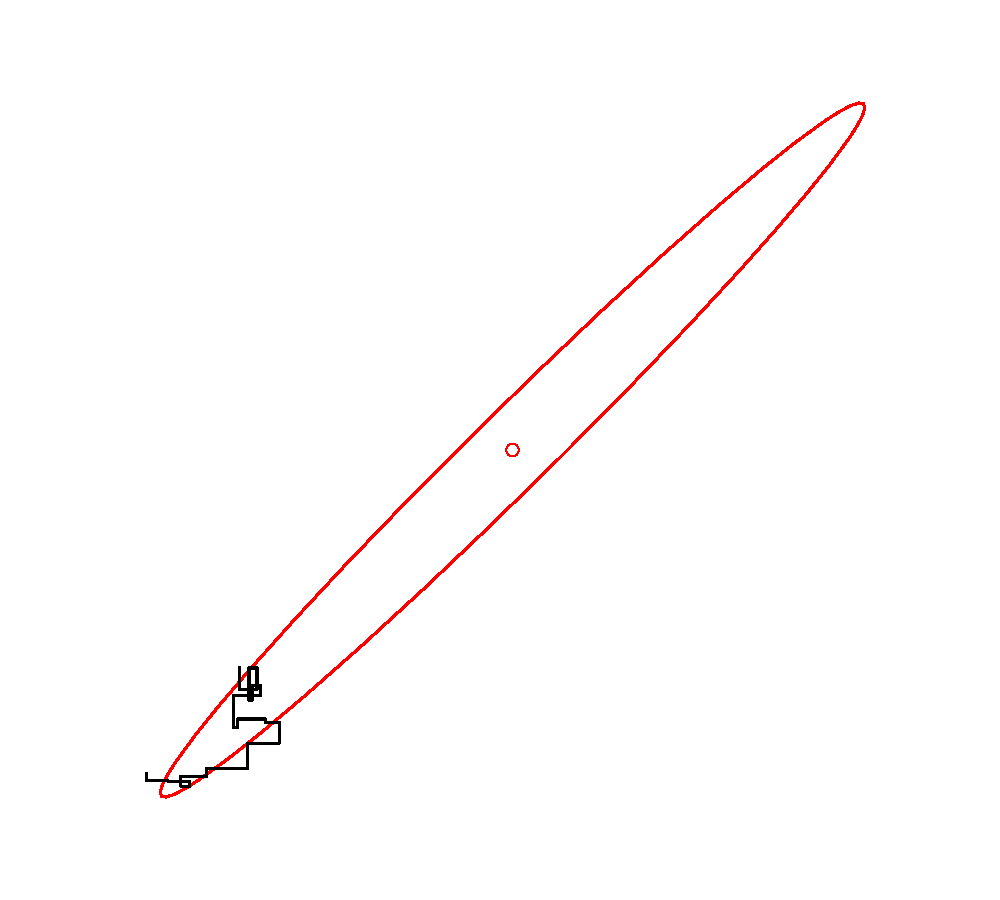
\includegraphics[height=3in]{poormixing.pdf}
\caption{An example of a poorly-mixing sample in two dimensions. Notice that the chain is trapped in a region of low probability relative to the mean (dot) and variance (oval) of the true posterior quantity.}
\label{fig:mix}
\end{center}
\end{figure}

\subsubsection\*{Informal Methods}

The most straightforward approach for assessing convergence is based on simply plotting and inspecting traces and histograms of the observed MCMC sample. If the trace of values for each of the stochastics exhibits asymptotic behaviour\footnote{Asymptotic behaviour implies that the variance and the mean value of the sample stays relatively constant over some arbitrary period.} over the last $m$ iterations, this may be satisfactory evidence for convergence. A similar approach involves plotting a histogram for every set of $k$ iterations (perhaps 50-100) beyond some burn-in threshold $n$; if the histograms are not visibly different among the sample intervals, this is some evidence for convergence. Note that such diagnostics should be carried out for each stochastic estimated by the MCMC algorithm, because convergent behaviour by one variable does not imply evidence for convergence for other variables in the model. An extension of this approach can be taken when multiple parallel chains are run, rather than just a single, long chain. In this case, the final values of $c$ chains run for $n$ iterations are plotted in a histogram; just as above, this is repeated every $k$ iterations thereafter, and the histograms of the endpoints are plotted again and compared to the previous histogram. This is repeated until consecutive histograms are indistinguishable.

\begin{figure}[h]
\begin{center}
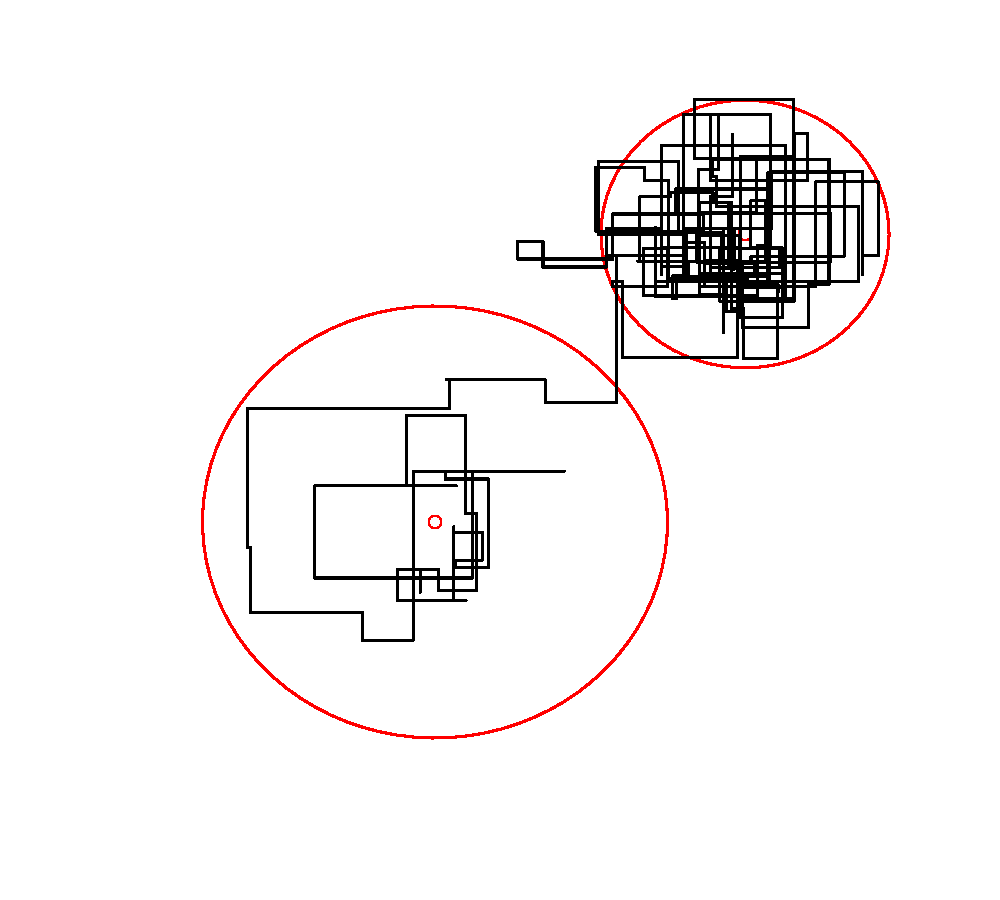
\includegraphics[height=3in]{metastable.pdf}
\caption{An example of metastability in a two-dimensional parameter space. The chain appears to be stable in one region of the parameter space for an extended period, then unpredictably jumps to another region of the space.}
\label{fig:metas}
\end{center}
\end{figure}

Another \emph{ad hoc} method for detecting convergence is to examine the traces of several MCMC chains initialized with different starting values. Overlaying these traces on the same set of axes should (if convergence has occurred) show each chain tending toward the same equilibrium value, with approximately the same variance. Recall that the tendency for some Markov chains to converge to the true (unknown) value from diverse initial values is called \emph{ergodicity}. This property is guaranteed by the reversible chains constructed using MCMC, and should be observable using this technique. Again, however, this approach is only a heuristic method, and cannot always detect lack of convergence, even though chains may appear ergodic.

A principal reason that evidence from informal techniques cannot guarantee convergence is a phenomenon called metastability. Chains may appear to have converged to the true equilibrium value, displaying excellent qualities by any of the methods described above. However, after some period of stability around this value, the chain may suddenly move to another region of the parameter space (Figure \ref{fig:metas}). This period of metastability can sometimes be very long, and therefore escape detection by these convergence diagnostics. Unfortunately, there is no statistical technique available for detecting metastability.

\subsubsection\*{Formal Methods}

Along with the \emph{ad hoc} techniques described above, a number of more formal methods exist which are prevalent in the literature. These are considered more formal because they are based on existing statistical methods, such as time series analysis.

\pkg{PyMC} currently includes functions for two formal convergence diagnostic procedures. The first, proposed by \citet{Geweke:1992gm}, is a time-series approach that compares the mean and variance of segments from the beginning and end of a single chain.
\begin{equation}
z = \frac{\bar{\theta}_a - \bar{\theta}_b}{\sqrt{Var(\theta_a) + Var(\theta_b)}}
\end{equation}
where $a$ is the early interval and $b$ the late interval. If the z-scores (theoretically distributed as standard normal variates) of these two segments are similar, it can provide evidence for convergence. \pkg{PyMC} calculates z-scores of the difference between various initial segments along the chain, and the last 50\% of the remaining chain. If the chain has converged, the majority of points should fall within 2 standard deviations of zero.

Diagnostic z-scores can be obtained by calling the \code{geweke} function. It accepts either (1) a single trace, (2) a Node or Stochastic object, or (3) an entire Model object.

\paragraph{Method Usage}
\begin{CodeInput}
\begin{CodeChunk}
pm.geweke(pymc_object, first=0.1, last=0.5, intervals=20)
\end{CodeChunk}
\end{CodeInput}
\begin{itemize}

\item \verb=pymc_object=: The object that is or contains the output trace(s).

\item \verb=first= (optional): First portion of chain to be used in Geweke diagnostic. Defaults to 0.1 (i.e. first 10\% of chain).

\item \verb=last= (optional): Last portion of chain to be used in Geweke diagnostic. Defaults to 0.5 (i.e. last 50\% of chain).

\item \verb=intervals= (optional): Number of sub-chains to analyze. Defaults to 20.
\end{itemize}

The resulting scores are best interpreted graphically, using the \code{geweke_plot} function. This displays the scores in series, in relation to the 2 standard deviation boundaries around zero. Hence, it is easy to see departures from the standard normal assumption.

\begin{figure}[h!]
\begin{center}
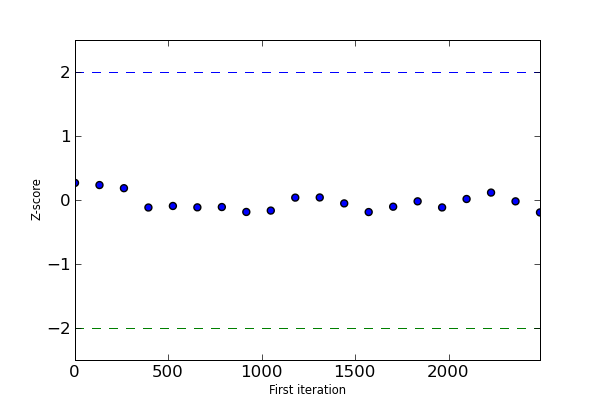
\includegraphics[height=6in]{geweke.png}
\caption{Sample plots of Geweke z-scores for a variable using \textbf{geweke_plot}. The occurrence of the scores well within 2 standard deviations of zero gives does not indicate lack of convergence (top), while deviations exceeding 2 standard deviations suggests that additional samples are required to achieve convergence (bottom).}
\label{fig:geweke}
\end{center}
\end{figure}

\code{geweke_plot} takes either a single set of scores, or a dictionary of scores (output by \code{geweke} when an entire Sampler is passed) as its argument:

\paragraph{Method Usage}
\begin{CodeInput}
\begin{CodeChunk}
geweke_plot(scores, name='geweke', format='png', suffix='-diagnostic', \
                path='./', fontmap = {1:10, 2:8, 3:6, 4:5, 5:4}, verbose=1)
\end{CodeChunk}
\end{CodeInput}
\begin{itemize}

\item \verb=scores=: The object that contains the Geweke scores. Can be a list (one set) or a dictionary (multiple sets).

\item \verb=name= (optional): Name used for output files. For multiple scores, the dictionary keys are used as names.

\item \verb=format= (optional): Graphic output file format (defaults to \emph{png}).

\item \verb=suffix= (optional): Suffix to filename (defaults to \emph{-diagnostic})

\item \verb=path= (optional): The path for output graphics (defaults to working directory).

\item \verb=fontmap= (optional): Dictionary containing the font map for the labels of the graphic.

\item \verb=verbose= (optional): Verbosity level for output (defaults to 1).
\end{itemize}

To illustrate, consider a model \code{my_model} that is used to instantiate a MCMC sampler. The sampler is then run for a given number of iterations:
\begin{CodeInput}
\begin{CodeChunk}
	>>> S = pm.MCMC(my_model)
	>>> S.sample(10000, burn=5000)
\end{CodeChunk}
\end{CodeInput}
It is easiest simply to pass the entire sampler \code{S} to the \code{geweke} function:
\begin{CodeInput}
\begin{CodeChunk}
	>>> scores = pm.geweke(S, intervals=20)
	>>> pm.Matplot.geweke_plot(scores)
\end{CodeChunk}
\end{CodeInput}
Alternatively, individual stochastics within \code{S} can be analyzed for convergence:
\begin{CodeInput}
\begin{CodeChunk}
	>>> trace = S.trace('alpha')[:]
	>>> alpha_scores = pm.geweke(trace, intervals=20)
	>>> pm.Matplot.geweke_plot(alpha_scores, 'alpha')
\end{CodeChunk}
\end{CodeInput}
An example of convergence and non-convergence of a chain using \code{geweke_plot} is given in Figure \ref{fig:geweke}. 


The second diagnostic provided by \pkg{PyMC} is the \citet{raftery} procedure. This approach estimates the number of iterations required to reach convergence, along with the number of burn-in samples to be discarded and the appropriate thinning interval. A separate estimate of both quantities can be obtained for each variable in a given model.

As the criterion for determining convergence, the Raftery and Lewis approach uses the accuracy of estimation of a user-specified quantile. For example, we may want to estimate the quantile $q=0.975$ to within $r=0.005$ with probability $s=0.95$. In other words,

\begin{equation}
	Pr(|\hat{q}-q| \le r) = s
\end{equation}

From any sample of $\theta$, one can construct a binary chain:

\begin{equation}
	Z^{(j)} = I(\theta^{(j)} \le u_q)
\end{equation}

where $u_q$ is the quantile value and $I$ is the indicator function. While $\{\theta^{(j)}\}$ is a Markov chain, $\{Z^{(j)}\}$ is not necessarily so. In any case, the serial dependency among $Z^{(j)}$ decreases as the thinning interval $k$ increases. A value of $k$ is chosen to be the smallest value such that the first order Markov chain is preferable to the second order Markov chain.

This thinned sample is used to determine number of burn-in samples. This is done by comparing the remaining samples from burn-in intervals of increasing length to the limiting distribution of the chain. An appropriate value is one for which the truncated sample's distribution is within $\epsilon$ (arbitrarily small) of the limiting distribution. See \citet{raftery} or \citet{Gamerman:1997tb} for computational details. Estimates for sample size tend to be conservative.

This diagnostic is best used on a short pilot run of a particular model, and the results used to parameterize a subsequent sample that is to be used for inference.


\paragraph{Method Usage}
\begin{CodeInput}
\begin{CodeChunk}
raftery_lewis(pymc_object, q, r, s=.95, epsilon=.001, verbose=1)
\end{CodeChunk}
\end{CodeInput}
\begin{itemize}

	\item \verb=pymc_object=: The object that contains the Geweke scores. Can be a list (one set) or a dictionary (multiple sets).

    \item \verb=q=: Desired quantile to be estimated.

    \item \verb=r=: Desired accuracy for quantile.

    \item \verb=s=(optional): Probability of attaining the requested accuracy (defaults to 0.95).

    \item \verb=epsilon= (optional) : Half width of the tolerance interval required for the q-quantile (defaults to 0.001).

    \item \verb=verbose= (optional) : Verbosity level for output (defaults to 1).
\end{itemize}

The code for \code{raftery_lewis} is based on the FORTRAN program \emph{gibbsit}, which was written by Steven Lewis.

For example, consider again a sampler \code{S} run for some model \code{my_model}:
\begin{CodeInput}
\begin{CodeChunk}
	>>> S = pm.MCMC(my_model)
	>>> S.sample(10000, burn=5000)
\end{CodeChunk}
\end{CodeInput}
One can pass either the entire sampler \code{S} or any stochastic within \code{S} to the \code{raftery_lewis} function, along with suitable arguments. Here, we have chosen $q=0.025$ (the lower limit of the equal-tailed 95\% interval) and error $r=0.01$:
\begin{CodeInput}
\begin{CodeChunk}
	>>> pm.raftery_lewis(S, q=0.025, r=0.01)
\end{CodeChunk}
\end{CodeInput}
This yields diagnostics as follows for each stochastic of \code{S}, as well as a dictionary containing the diagnostic quantities:

\begin{CodeInput}
\begin{CodeChunk}
	========================
	Raftery-Lewis Diagnostic
	========================

	937 iterations required (assuming independence) to achieve 0.01 accuracy
	with 95 percent probability.

	Thinning factor of 1 required to produce a first-order Markov chain.

	39 iterations to be discarded at the beginning of the simulation (burn-in).

	11380 subsequent iterations required.

	Thinning factor of 11 required to produce an independence chain.
\end{CodeChunk}
\end{CodeInput}

Additional convergence diagnostics are available in the
\href{http://lib.stat.cmu.edu/R/CRAN/}{R statistical package}, via the
\href{http://www-fis.iarc.fr/coda/}{CODA module}. \pkg{PyMC} includes a method
\code{coda} for exporting model traces in a format that may be
directly read by CODA.

\paragraph{Method Usage}
\begin{CodeInput}
\begin{CodeChunk}
pm.utils.coda(pymc_object)
\end{CodeChunk}
\end{CodeInput}
\begin{itemize}

\item \verb=pymc_object=: The \pkg{PyMC} sampler for which output is desired.

\end{itemize}
Calling \verb=coda= yields two files, one containing raw trace values (suffix
\verb=.out=) and another containing indices to the trace values (suffix
\verb=.ind=).

% Section~convergence_diagnostics (end)

\subsubsection\*{Autocorrelation Plots} % (fold)
%\label{sec:autocorrelation_plots}

Samples from MCMC algorithms are ususally autocorrelated, due partly to the
inherent Markovian dependence structure. The degree of autocorrelation can
be quantified using the autocorrelation function:
\begin{eqnarray*}
    \rho_k &=& \frac{\mbox{Cov}(X_t,
X_{t+k})}{\sqrt{\mbox{Var}(X_t)\mbox{Var}(X_{t+k})}} \\
            &=& \frac{E[(X_t - \theta)(X_{t+k} - \theta)]}{\sqrt{E[(X_t -
\theta)^2] E[(X_{t+k} - \theta)^2]}}
\end{eqnarray*}
\pkg{PyMC} includes a function for plotting the autocorrelation function for each
stochastic in the sampler (Figure \ref{fig:autocorr}). This allows users
to examine the relationship among successive samples within sampled chains.
Significant autocorrelation suggests that chains require thinning prior to
use of the posterior statistics for inference.

\begin{figure}[h]
        \begin{center}
        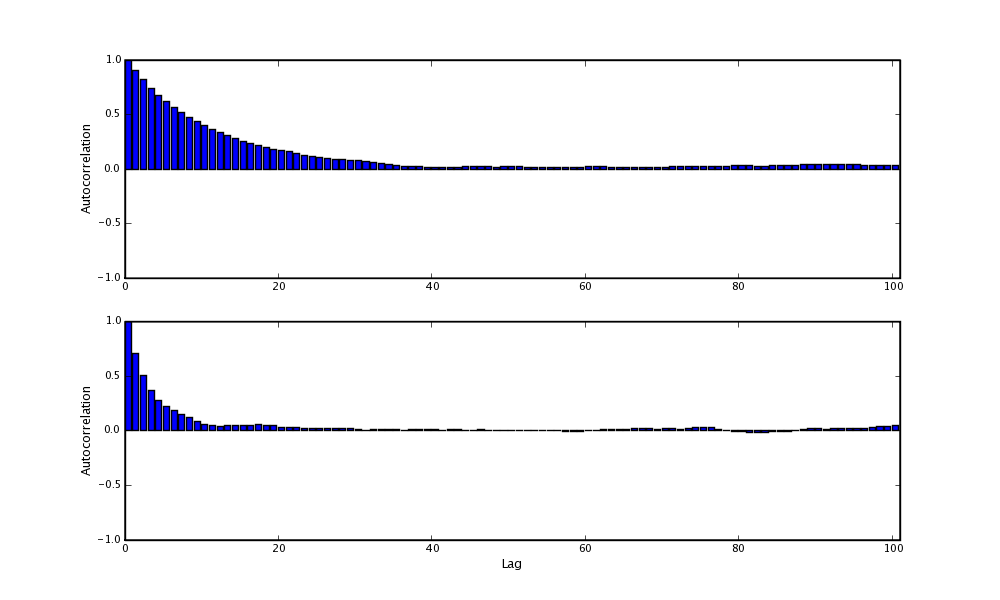
\includegraphics[scale=0.4]{autocorr.png}
    \end{center}
    \caption{Sample autocorrelation plots for two Poisson variables from
coal mining disasters example model.}
    \label{fig:autocorr}
\end{figure}

\begin{CodeInput}
\begin{CodeChunk}
autocorrelation(pymc_object, name, maxlag=100, format='png', suffix='-acf',
path='./', fontmap = {1:10, 2:8, 3:6, 4:5, 5:4}, verbose=1)
\end{CodeChunk}
\end{CodeInput}
\begin{itemize}
	\item \verb=pymc_object=: The object that is or contains the output
trace(s).

	\item \verb=name=: Name used for output files.

	\item \verb=maxlag=: The highest lag interval for which
autocorrelation is calculated.

	\item \verb=format= (optional): Graphic output file format
(defaults to \emph{png}).

	\item \verb=suffix= (optional): Suffix to filename (defaults to
\emph{-diagnostic})

	\item \verb=path= (optional): The path for output graphics
(defaults to working directory).

	\item \verb=fontmap= (optional): Dictionary containing the font map
for the labels of the graphic.

	\item \verb=verbose= (optional): Verbosity level for output
(defaults to 1).
\end{itemize}

Using any given model \code{my_model} as an example, autocorrelation plots can be obtained simply by passing the sampler for that model to the \code{autocorrelation} function (within the \code{Matplot} module) directly:
\begin{CodeInput}
\begin{CodeChunk}
	>>> S = pm.MCMC(my_model)
	>>> S.sample(10000, burn=5000)
	>>> pm.Matplot.autocorrelation(S)
\end{CodeChunk}
\end{CodeInput}
Alternatively, variables within a model can be plotted individually. For example, a hypothetical variable \code{beta} that was estimated using sampler \code{S} will yield a correlation plot as follows:
\begin{CodeInput}
\begin{CodeChunk}
	>>> pm.Matplot.autocorrelation(S.beta)
\end{CodeChunk}
\end{CodeInput}

% Section~autocorrelation_plots (end)

\subsection{Goodness of Fit} % (fold)
%\label{sec:goodness_of_fit}

Checking for model convergence is only the first step in the evaluation of MCMC model outputs. It is possible for an entirely unsuitable model to converge, so additional steps are needed to ensure that the estimated model adequately fits the data. One intuitive way for evaluating model fit is to compare model predictions with actual observations. In other words, the fitted model can be used to simulate data, and the distribution of the simulated data should resemble the distribution of the actual data.

Fortunately, simulating data from the model is a natural component of the Bayesian modelling framework. Recall, from the discussion on imputation of missing data, the posterior predictive distribution:

\begin{equation}
	p(\tilde{y}|y) = \int p(\tilde{y}|\theta) f(\theta|y) d\theta
\end{equation}

Here, $\tilde{y}$ represents some hypothetical new data that would be expected, taking into account the posterior uncertainty in the model parameters. Sampling from the posterior predictive distribution is easy in \pkg{PyMC}. The code looks identical to the corresponding data stochastic, with two modifications: (1) the node should be specified as deterministic and (2) the statistical likelihoods should be replaced by random number generators. As an example, consider a simple dose-response model, where deaths are modeled as a binomial random variable for which the probability of death is a logit-linear function of the dose of a particular drug:
\begin{CodeInput}
\begin{CodeChunk}
	# Sample size, dose and response
	n = [5]*4
	dose = [-.86,-.3,-.05,.73]
	x = [0,1,3,5]

	alpha = pm.Normal('alpha', mu=0.0, tau=0.01)
	beta = pm.Normal('beta', mu=0.0, tau=0.01)

	@pm.deterministic
	def theta(a=alpha, b=beta, d=dose):
	    """theta = inv_logit(a+b)"""
	    return pm.invlogit(a+b*d)

	"""deaths ~ binomial(n, p)"""
	deaths = pm.Binomial('deaths', n=n, p=theta, value=x, observed=True)
\end{CodeChunk}
\end{CodeInput}
The posterior predictive distribution of deaths uses the same functional form as the data likelihood, in this case a binomial stochastic. Here is the corresponding sample from the posterior predictive distribution:
\begin{CodeInput}
\begin{CodeChunk}
	@pm.deterministic
	def deaths_sim(n=n, p=theta):
	    """deaths_sim = rbinomial(n, p)"""
	    return pm.rbinomial(n, p)
\end{CodeChunk}
\end{CodeInput}
Notice that the stochastic \code{pm.Binomial} has been replaced with a deterministic node that simulates values using \code{pm.rbinomial} and the unknown parameters \code{theta}. 

The degree to which simulated data correspond to observations can be evaluated in at least two ways. First, these quantities can simply be compared visually. This allows for a qualitative comparison of model-based replicates and observations. If there is poor fit, the true value of the data may appear in the tails of the histogram of replicated data, while a good fit will tend to show the true data in high-probability regions of the posterior predictive distribution (Figure~\ref{fig:gof}).

\begin{figure}[htdevi!]
        \begin{center}
        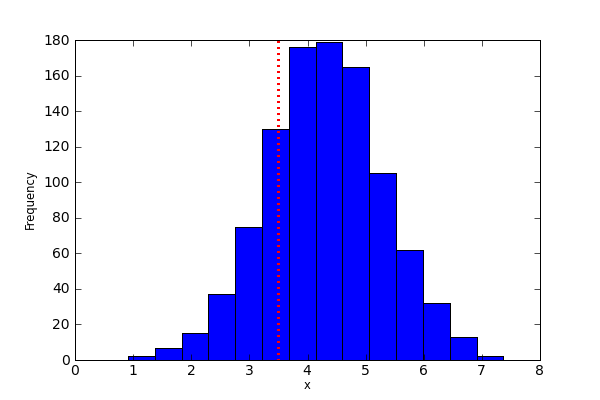
\includegraphics[height=3in]{gof.png}
    \end{center}
    \caption{Data sampled from the posterior predictive distribution of a model for some observation \textbf{x}. The true value of \textbf{x} is shown by the dotted red line.}
    \label{fig:gof}
\end{figure}

The Matplot module in \pkg{PyMC} provides an easy way of producing such plots, via the \code{gof_plot} function. To illustrate, consider a single observed data point \code{x} and an array of values \code{x_sim} sampled from the posterior predictive distribution. The histogram is generated by calling:

\begin{CodeInput}
\begin{CodeChunk}
	pm.Matplot.gof_plot(x_sim, x, name='x')
\end{CodeChunk}
\end{CodeInput}

A second approach for evaluating goodness of fit using samples from the posterior predictive distribution involves the use of a statistical criterion. For example, the Bayesian p-value \citep{Gelman:1996gp} uses a discrepancy measure that quantifies the difference between data (observed or simulated) $x$ and the expected value $e$, conditional on some model. One such discrepancy measure is the Freeman-Tukey statistic \citep{Brooks:2000il}:

\begin{equation}
	D(x|\theta) = \sum_j (\sqrt{x_j}-\sqrt{e_j})^2
\end{equation}

Model fit is assessed by comparing the discrepancies from observed data to those from simulated data. On average, we expect the difference between them to be zero; hence, the Bayesian p-value is simply the proportion of simulated discrepancies that are larger than their corresponding observed discrepancies:

\begin{equation}
	p = Pr[ D(\text{sim}) > D(\text{obs}) ]
\end{equation}

If $p$ is very large (e.g. $>0.975$) or very small (e.g. $<0.025$) this implies that the model is not consistent with the data, and thus is evidence of lack of fit. Graphically, data and simulated discrepancies plotted together should be clustered along a 45 degree line passing through the origin, as shown in Figure~\ref{fig:deviate}.

\begin{figure}[ht!]
        \begin{center}
        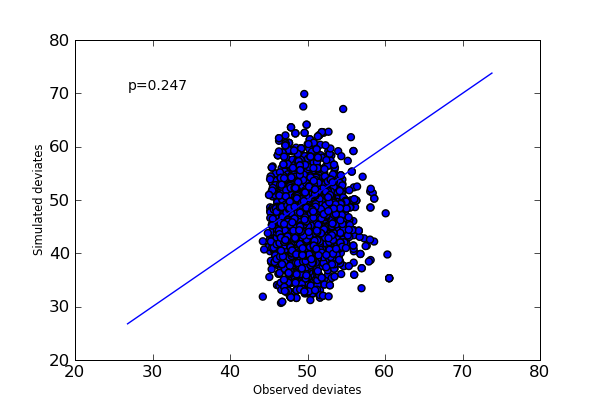
\includegraphics[height=3in]{deviates.png}
    \end{center}
    \caption{Plot of deviates of observed and simulated data from expected values. The cluster of points symmetrically about the 45 degree line (and the reported p-value) suggests acceptable fit for the modeled parameter.}
    \label{fig:deviate}
\end{figure}

The \code{discrepancy} function in the \code{diagnostics} module can be used to generate discrepancy statistics from arrays of data, simulated values, and expected values:

\begin{CodeInput}
\begin{CodeChunk}
	D = pm.diagnostics.discrepancy(x, x_sim, x_exp)
\end{CodeChunk}
\end{CodeInput}

A call to this function returns two arrays of discrepancy values (one for observed data and one for simulated data), which can be passed to the \code{discrepancy_plot} function in the Matplot module to generate a scatter plot, and if desired, a p-value:

\begin{CodeInput}
\begin{CodeChunk}
	pm.Matplot.discrepancy_plot(D, name='D', report_p=True)
\end{CodeChunk}
\end{CodeInput}

Additional optional arguments for \code{discrepancy_plot} are identical to other \pkg{PyMC} plotting functions.

% Section~goodness_of_fit (end)




\section[Extending PyMC]{Extending \pkg{PyMC}}
\label{chap:extending}
\pkg{PyMC} tries to make standard things easy, but keep unusual things possible. Its openness, combined with \proglang{Python}'s flexibility, invite extensions from using new step methods to exotic stochastic processes (see the Gaussian process module). This Section~briefly reviews the ways \pkg{PyMC} is designed to be extended.


\subsection{Nonstandard Stochastics} \label{nonstandard}


The simplest way to create a \code{Stochastic} object with a nonstandard distribution is to use the medium or long decorator syntax. See Section~\ref{chap:modelbuilding}. If you want to create many stochastics with the same nonstandard distribution, the decorator syntax can become cumbersome. An actual subclass of \code{Stochastic} can be created using the class factory \code{stochastic_from_dist}. This function takes the following arguments:
\begin{itemize}
   \item The name of the new class,
   \item A \code{logp} function,
   \item A \code{random} function (which may be \code{None}),
   \item The \pkg{NumPy} datatype of the new class (for continuous distributions, this should be \code{float}; for discrete distributions, \code{int}; for variables valued as non-numerical objects, \code{object}),
   \item A flag indicating whether the resulting class represents a vector-valued variable.
\end{itemize}
The necessary parent labels are read from the \code{logp} function, and a docstring for the new class is automatically generated.

Full subclasses of \code{Stochastic} may be necessary to provide nonstandard behaviors (see \code{gp.GP}).


\subsection{User-defined step methods} \label{custom-stepper}

The \code{StepMethod} class is meant to be subclassed. There are an enormous number of MCMC step methods in the literature, whereas \pkg{PyMC} provides only about half a dozen. Most user-defined step methods will be either Metropolis-Hastings or Gibbs step methods, and these should subclass \code{Metropolis} or \code{Gibbs} respectively. More unusual step methods should subclass \code{StepMethod} directly.


\subsubsection\*{Example: an asymmetric Metropolis step} \label{user-gen}
Consider the probability model in \code{examples/custom_step.py}:
\begin{CodeInput}
\begin{CodeChunk}
mu = pymc.Normal('mu',0,.01, value=0)
tau = pymc.Exponential('tau',.01, value=1)
cutoff = pymc.Exponential('cutoff',1, value=1.3)
D = pymc.TruncatedNormal('D',mu,tau,-numpy.inf,cutoff,value=data,observed=True)
\end{CodeChunk}
\end{CodeInput}
The stochastic variable \code{cutoff} cannot be smaller than the largest element of $D$, otherwise $D$'s density would be zero. The standard \code{Metropolis} step method can handle this case without problems; it will propose illegal values occasionally, but these will be rejected.

\medskip
Suppose we want to handle \code{cutoff} with a smarter step method that doesn't propose illegal values. Specifically, we want to use the nonsymmetric proposal distribution
\begin{eqnarray*}
	x_p | x \sim \textup{Truncnorm}(x, \sigma, \max(D), \infty).
\end{eqnarray*}
We can implement this Metropolis-Hastings algorithm with the following step method class:
\begin{CodeInput}
\begin{CodeChunk}
class TruncatedMetropolis(pymc.Metropolis):
    def __init__(self, stochastic, low_bound, up_bound, *args, **kwargs):
        self.low_bound = low_bound
        self.up_bound = up_bound
        pymc.Metropolis.__init__(self, stochastic, *args, **kwargs)

    # Propose method generates proposal values
    def propose(self):
        tau = 1./(self.adaptive_scale_factor * self.proposal_sd)**2
        self.stochastic.value = \
            pymc.rtruncnorm(self.stochastic.value, tau, self.low_bound, self.up_bound)

    # Hastings factor method accounts for asymmetric proposal distribution
    def hastings_factor(self):
        tau = 1./(self.adaptive_scale_factor * self.proposal_sd)**2
        cur_val = self.stochastic.value
        last_val = self.stochastic.last_value

        lp_for = pymc.truncnorm_like(cur_val, last_val, tau, self.low_bound, self.up_bound)
        lp_bak = pymc.truncnorm_like(last_val, cur_val, tau, self.low_bound, self.up_bound)

        if self.verbose > 1:
            print self._id + ': Hastings factor %f'%(lp_bak - lp_for)
        return lp_bak - lp_for
\end{CodeChunk}
\end{CodeInput}

The \code{propose} method sets the step method's stochastic's value to a new value, drawn from a truncated normal distribution. The precision of this distribution is computed from two factors: \code{self.proposal_sd}, which can be set with an input argument to Metropolis, and \code{self.adaptive_scale_factor}. Metropolis step methods' default tuning behavior is to reduce \code{adaptive_scale_factor} if the acceptance rate is too low, and to increase \code{adaptive_scale_factor} if it is too high. By incorporating \code{adaptive_scale_factor} into the proposal standard deviation, we avoid having to write our own tuning infrastructure. If we don't want the proposal to tune, we don't have to use \code{adaptive_scale_factor}.

The \code{hastings_factor} method adjusts for the asymmetric proposal distribution \citep{gelman}. It computes the log of the quotient of the `backward' density and the `forward' density. For symmetric proposal distributions, this quotient is 1, so its log is zero. 

\medskip
Having created our custom step method, we need to tell MCMC instances to use it to handle the variable \code{cutoff}. This is done in \code{custom_step.py} with the following line:
\begin{CodeInput}
\begin{CodeChunk}
M.use_step_method(TruncatedMetropolis, cutoff, D.value.max(), numpy.inf)
\end{CodeChunk}
\end{CodeInput}
This call causes $M$ to pass the arguments \code{cutoff, D.value.max(), numpy.inf} to a \code{TruncatedMetropolis} object's \code{init} method, and use the object to handle \code{cutoff}.

\medskip
It's often convenient to get a handle to a custom step method instance directly for debugging purposes. \code{M.step_method_dict[cutoff]} returns a list of all the step methods $M$ will use to handle \code{cutoff}:
\begin{CodeInput}
\begin{CodeChunk}
>>> M.step_method_dict[cutoff]
[<custom_step.TruncatedMetropolis object at 0x3c91130>]
\end{CodeChunk}
\end{CodeInput}
There may be more than one, and conversely step methods may handle more than one stochastic variable. To see which variables step method $S$ is handling, try
\begin{CodeInput}
\begin{CodeChunk}
>>> S.stochastics
set([<pymc.distributions.Exponential 'cutoff' at 0x3cd6b90>])
\end{CodeChunk}
\end{CodeInput}


\subsubsection\*{General step methods} \label{user-gen}


All step methods must implement the following methods:
\begin{description}
   \item[\code{step()}:] Updates the values of \code{self.stochastics}.
   \item[\code{tune()}:] Tunes the jumping strategy based on performance so far. A default method is available that increases \code{self.adaptive_scale_factor} (see below) when acceptance rate is high, and decreases it when acceptance rate is low. This method should return \code{True} if additional tuning will be required later, and \code{False} otherwise.
   \item[\code{competence(s):}] A class method that examines stochastic variable $s$ and returns a value from 0 to 3 expressing the step method's ability to handle the variable. This method is used by \code{MCMC} instances when automatically assigning step methods. Conventions are:
   \begin{description}
      \item[0] I cannot safely handle this variable.
      \item[1] I can handle the variable about as well as the standard \code{Metropolis} step method.
      \item[2] I can do better than \code{Metropolis}.
      \item[3] I am the best step method you are likely to find for this variable in most cases.
   \end{description}
   For example, if you write a step method that can handle \code{NewStochasticSubclass} well, the competence method might look like this:
\begin{CodeInput}
\begin{CodeChunk}
class NewStepMethod(pymc.StepMethod):
   def __init__(self, stochastic, *args, **kwargs):
      ...

   @classmethod
   def competence(self, stochastic):
      if isinstance(stochastic, NewStochasticSubclass):
         return 3
      else:
         return 0
\end{CodeChunk}
\end{CodeInput}
   Note that \pkg{PyMC} will not even attempt to assign a step method automatically if its \code{init} method cannot be called with a single stochastic instance, that is \code{NewStepMethod(x)} is a legal call. The list of step methods that \pkg{PyMC} will consider assigning automatically is called \code{pymc.StepMethodRegistry}.
   \item[\code{current_state()}:] This method is easiest to explain by showing the code:
   \begin{CodeInput}
\begin{CodeChunk}
state = {}
for s in self._state:
    state[s] = getattr(self, s)
return state
   \end{CodeChunk}
\end{CodeInput}
   \code{self._state} should be a list containing the names of the attributes needed to reproduce the current jumping strategy. If an \code{MCMC} object writes its state out to a database, these attributes will be preserved. If an \code{MCMC} object restores its state from that database later, the corresponding step method will have these attributes set to their saved values.
\end{description}

Step methods should also maintain the following attributes:
\begin{description}
   \item[\code{_id}:] A string that can identify each step method uniquely (usually something like \code{<class_name>_<stochastic_name>}).
   \item[\code{adaptive_scale_factor}:] An `adaptive scale factor'. This attribute is only needed if the default \code{tune()} method is used.
   \item[\code{_tuning_info}:] A list of strings giving the names of any tuning parameters. For \code{Metropolis} instances, this would be \code{['adaptive_scale_factor']}. This list is used to keep traces of tuning parameters in order to verify `diminishing tuning' \citep{tuning}.
\end{description}

All step methods have a property called \code{loglike}, which gives the sum of the log-probabilities of the union of the extended children of \code{self.stochastics}. This quantity is one term in the log of the Metropolis-Hastings acceptance ratio. The \code{logp_plus_loglike} property gives the sum of that and the log-probabilities of \code{self.stochastics}.  



\subsubsection\*{Metropolis-Hastings step methods} \label{user-metro}

A Metropolis-Hastings step method only needs to implement the following methods, which are called by \code{Metropolis.step()}:
\begin{description}
   \item[\code{reject()}:] Usually just
   \begin{CodeInput}
\begin{CodeChunk}
def reject(self):
    self.rejected += 1
    [s.value = s.last_value for s in self.stochastics]
   \end{CodeChunk}
\end{CodeInput}
   \item[\code{propose():}] Sets the values of all \code{self.stochastics} to new, proposed values. This method may use the \code{adaptive_scale_factor} attribute to take advantage of the standard tuning scheme.
\end{description}
Metropolis-Hastings step methods may also override the \code{tune} and \code{competence} methods.

Metropolis-Hastings step methods with asymmetric jumping distributions must implement a method called \code{hastings_factor()}, which returns the log of the ratio of the `reverse' and `forward' proposal probabilities. Note that no \code{accept()} method is needed or used.

Metropolis-Hastings step methods should log the number of jumps they have accepted and rejected using attributes called \code{accepted} and \code{rejected}.


\subsubsection\*{Gibbs step methods} \label{user-gibbs}


Gibbs step methods handle conjugate submodels. These models usually have two components: the `parent' and the `children'. For example, a gamma-distributed variable serving as the precision of several normally-distributed variables is a conjugate submodel; the gamma variable is the parent and the normal variables are the children.

This Section~describes \pkg{PyMC}'s current scheme for Gibbs step methods, several of which are in a semi-working state in the sandbox. It is meant to be as generic as possible to minimize code duplication, but it is admittedly complicated. Feel free to subclass StepMethod directly when writing Gibbs step methods if you prefer.

Gibbs step methods that subclass \pkg{PyMC}'s \code{Gibbs} should define the following class attributes:
\begin{description}
   \item[\code{child_class}:] The class of the children in the submodels the step method can handle.
   \item[\code{parent_class}:] The class of the parent.
   \item[\code{parent_label}:] The label the children would apply to the parent in a conjugate submodel. In the gamma-normal example, this would be \code{tau}.
   \item[\code{linear_OK}:] A flag indicating whether the children can use linear combinations involving the parent as their actual parent without destroying the conjugacy.
\end{description}

A subclass of \code{Gibbs} that defines these attributes only needs to implement a \code{propose()} method, which will be called by \code{Gibbs.step()}. The resulting step method will be able to handle both conjugate and `non-conjugate' cases. The conjugate case corresponds to an actual conjugate submodel. In the nonconjugate case all the children are of the required class, but the parent is not. In this case the parent's value is proposed from the likelihood and accepted based on its prior. The acceptance rate in the nonconjugate case will be less than one.

The inherited class method \code{Gibbs.competence} will determine the new step method's ability to handle a variable $x$ by checking whether:
\begin{itemize}
   \item all $x$'s children are of class \code{child_class}, and either apply \code{parent_label} to $x$ directly or (if \code{linear_OK=True}) to a \code{LinearCombination} object (Section~\ref{chap:modelbuilding}), one of whose parents contains $x$.
   \item $x$ is of class \code{parent_class}
\end{itemize}
If both conditions are met, \code{pymc.conjugate_Gibbs_competence} will be returned. If only the first is met, \code{pymc.nonconjugate_Gibbs_competence} will be returned.


\subsection{New fitting algorithms} \label{custom-model}


\pkg{PyMC} provides a convenient platform for non-MCMC fitting algorithms in addition to MCMC. All fitting algorithms should be implemented by subclasses of \code{Model}. There are virtually no restrictions on fitting algorithms, but many of \code{Model}'s behaviors may be useful. See Section~\ref{chap:modelfitting}.


\subsubsection\*{Monte Carlo fitting algorithms} \label{custom-MC}


Unless there is a good reason to do otherwise, Monte Carlo fitting algorithms should be implemented by subclasses of \code{Sampler} to take advantage of the interactive sampling feature and database backends. Subclasses using the standard \code{sample()} and \code{isample()} methods must define one of two methods:
\begin{description}
   \item[\code{draw()}:] If it is possible to generate an independent sample from the posterior at every iteration, the \code{draw} method should do so. The default \code{_loop} method can be used in this case.
   \item[\code{_loop()}:] If it is not possible to implement a \code{draw()} method, but you want to take advantage of the interactive sampling option, you should override \code{_loop()}. This method is responsible for generating the posterior samples and calling \code{tally()} when it is appropriate to save the model's state. In addition, \code{_loop} should monitor the sampler's \code{status} attribute at every iteration and respond appropriately. The possible values of \code{status} are:
   \begin{description}
      \item[\code{'ready'}:] Ready to sample.
      \item[\code{'running'}:] Sampling should continue as normal.
      \item[\code{'halt'}:] Sampling should halt as soon as possible. \code{_loop} should call the \code{halt()} method and return control. \code{_loop} can set the status to \code{'halt'} itself if appropriate (eg the database is full or a \code{KeyboardInterrupt} has been caught).
      \item[\code{'paused'}:] Sampling should pause as soon as possible. \code{_loop} should return, but should be able to pick up where it left off next time it's called.
   \end{description}
\end{description}

Samplers may alternatively want to override the default \code{sample()} method. In that case, they should call the \code{tally()} method whenever it is appropriate to save the current model state. Like custom \code{_loop()} methods, custom \code{sample()} methods should handle \code{KeyboardInterrupts} and call the \code{halt()} method when sampling terminates to finalize the traces.


\subsection{Don't update stochastic variables' values in-place}
\label{dont-update-indepth}


If you're going to implement a new step method, fitting algorithm or unusual (non-numeric-valued) \code{Stochastic} subclass, you should understand the issues related to in-place updates of \code{Stochastic} objects' values. Fitting methods should never update variables' values in-place for two reasons:
\begin{itemize}
   \item In algorithms that involve accepting and rejecting proposals, the `pre-proposal' value needs to be preserved uncorrupted. It would be possible to make a copy of the pre-proposal value and then allow in-place updates, but in \pkg{PyMC} we have chosen to store the pre-proposal value as \code{Stochastic.last_value} and require proposed values to be new objects. In-place updates would corrupt \code{Stochastic.last_value}, and this would cause problems.
   \item \code{LazyFunction}'s caching scheme checks variables' current values against its internal cache by reference. That means if you update a variable's value in-place, it or its child may miss the update and incorrectly skip recomputing its value or log-probability.
\end{itemize}

However, a \code{Stochastic} object's value can make in-place updates to itself if the updates don't change its identity. For example, the \code{Stochastic} subclass \code{gp.GP} is valued as a \code{gp.Realization} object. GP realizations represent random functions, which are infinite-dimensional stochastic processes, as literally as possible. The strategy they employ is to `self-discover' on demand: when they are evaluated, they generate the required value conditional on previous evaluations and then make an internal note of it. This is an in-place update, but it is done to provide the same interface as a single random function whose value everywhere has been determined since it was created.


\clearpage

\section{Conclusion}
\label{conclusion}
%!TEX root = UserGuide.tex

MCMC is a surprisingly difficult and bug-prone algorithm to implement by hand. We find \pkg{PyMC} makes it much easier and less stressful. \pkg{PyMC} also makes our work more dynamic; getting hand-coded MCMC's working used to be so much work that we were reluctant to change anything, but with \pkg{PyMC} changing models is a breeze. We hope it does the same for you!

% \hypertarget{whatsnext}{}
% \subsection{What's next?} % (fold)
% 
% 
% A partial list of the features we would like to include in future releases follows. Three stars means that only debugging and checking is needed, so the feature is likely to be available in release 2.1; two stars means that there are no conceptual hurdles to be overcome but there's a lot of work left to do; and one star means only experimental development has been done.
% \begin{itemize}
%    \item (***) Gibbs step methods to handle conjugate and nearly-conjugate submodels,
%    \item (***) Handling all-normal submodels with sparse linear algebra \citep{normalsubmodel}. This will help \pkg{PyMC} handle Markov random fields and time-series models based on the `dynamic linear model' \citep{westharrison} (among others) more efficiently, in some cases fitting them in closed form,
%    \item (**) Generic Monte Carlo EM and SEM algorithms,
%    \item (**) Parallelizing single chains with a thread pool,
%    \item (**) Terse syntax inspired by \cite{fbc} for creating variables: \code{C=A*B} should return a deterministic object if $A$ and/or $B$ is a \pkg{PyMC} variable,
%    \item (**) Distributing multiple chains across multiple processes,
%    \item (*) Parsers for model-definition syntax from R and WinBugs,
%    \item (*) Dirichlet processes and other stick-breaking processes \citep{stickbreak}.
% \end{itemize}
% These features will make their way into future releases as (and if) we are able to finish them and make them reliable.

\subsection{How to get involved} % (fold)

We welcome new contributors at all levels. If you would like to contribute new code, improve documentation, share your results or provide ideas for new features, please introduce yourself on our \href{pymc@googlegroups.com}{mailing list}. Our \href{http://code.google.com/p/pymc/w/list}{wiki page} also hosts a number of tutorials and examples from users that could give you some ideas. We have taken great care to make the code easy to extend, whether by adding new database backends, step methods or entirely new sampling algorithms. Contributing to open source projects is a great experience, so don't hesitate to jump in and become part of \pkg{PyMC} !   





\section[Acknowledgments]{Acknowledgments}
\label{chap:acknowledge}
The authors would like to thank several users of \pkg{PyMC} who have been particularly helpful during the development of the 2.0 release. In alphabetical order, these are Mike Conroy, Abraham Flaxman, J. Miguel Marin, Aaron MacNeil, Nick Matsakis, John Salvatier and Andrew Straw.

Anand Patil's work on \pkg{PyMC} has been supported since 2008 by the \href{http://www.map.ox.ac.uk}{Malaria Atlas
Project}, principally funded by the Wellcome Trust.

David Huard's early work on \pkg{PyMC} was supported by a scholarship from the Natural Sciences and Engineering Research Council of Canada. 
\newpage
\appendix
% \section[MCMC]{Markov chain Monte Carlo}
% \label{sec:MCMC}
% %!TEX root = guide2.0.tex

\hypertarget{monte-carlo-methods-in-bayesian-analysis}{}


\subsection{Monte Carlo Methods in Bayesian Analysis}

Bayesian analysis often requires integration over multiple dimensions that is intractable both via analytic methods or standard methods of numerical integration. However, it is often possible to compute these integrals by simulating (drawing samples) from posterior distributions. For example, consider the expected value of a random variable $\mathbf{x}$:

\[
E[{\bf x}] = \int {\bf x} f({\bf x}) d{\bf x}, \qquad
{\bf x} = \{x_1,...,x_k\}
\]

\noindent where $k$ (the dimension of vector $x$) is perhaps very large. If we can produce a reasonable number of random vectors $\{{\bf x_i}\}$, we can use these values to approximate the unknown integral. This process is known as {\em Monte Carlo integration}. In general, MC integration allows integrals against probability density functions:

\[
I = \int h(\mathbf{x}) f(\mathbf{x}) \mathbf{dx}
\]

\noindent to be estimated by finite sums:

\[
\hat{I} = \frac{1}{n}\sum_{i=1}^n h(\mathbf{x}_i),
\]

\noindent where $\mathbf{x}_i$ is a sample from $f$. This estimate is valid and useful because:

\begin{itemize}
\item
By the strong law of large numbers:
\[\hat{I} \rightarrow I   \mbox{   with probability 1}\]
\item
Simulation error can be measured and controlled:
\[Var(\hat{I}) = \frac{1}{n(n-1)}\sum_{i=1}^n (h(\mathbf{x}_i)-\hat{I})^2\]
\end{itemize}

Why is this relevant to Bayesian analysis? If we replace $f(\mathbf{x})$ with a posterior, $f(\theta|d)$ and make $h(\theta)$ an interesting function of the unknown parameter, the resulting expectation is that of the posterior of $h(\theta)$:

\[
E[h(\theta)|d] = \int f(\theta|d) h(\theta) d\theta \approx \frac{1}{n}\sum_{i=1}^n h(\theta)
\]

%___________________________________________________________________________

\hypertarget{rejection-sampling}{}

\subsubsection\*{Rejection Sampling}

Though Monte Carlo integration allows us to estimate integrals that are unassailable by analysis and standard numerical methods, it relies on the ability to draw samples from the posterior distribution. For known parametric forms, this is not a problem; probability integral transforms or bivariate techniques (e.g Box-Muller method) may be used to obtain samples from uniform pseudo-random variates generated from a computer. Often, however, we cannot readily generate random values from non-standard posteriors. In such instances, we can use rejection sampling to generate samples.

\begin{figure}[ht]
        \begin{center}
        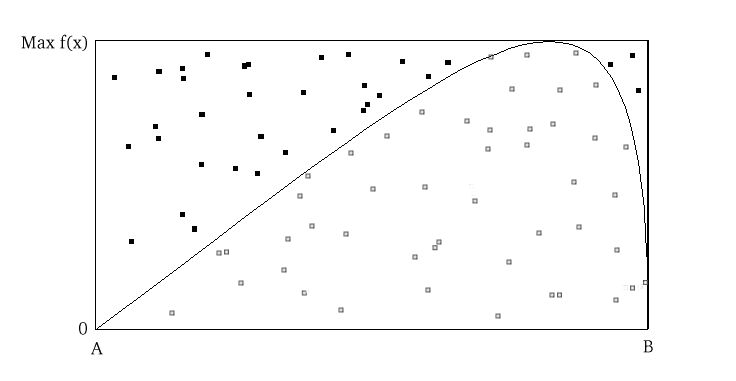
\includegraphics[scale=0.4]{reject.png}
    \end{center}
    \caption{Rejection sampling of a bounded form. Area is estimated by the ratio of accepted (open squares) to total points, multiplied by the rectangle area.}
    \label{fig:bound}
\end{figure}

Posit a function, $f(x)$ which can be evaluated for any value on the support of $x:S_x = [A,B]$, but may not be integrable or easily sampled from. If we can calculate the maximum  value of $f(x)$, we can then define a rectangle that is guaranteed to contain all possible values $(x,f(x))$. It is then trivial to generate points over the box and enumerate the values that fall under the curve (Figure \ref{fig:bound}).

\[
\frac{\mbox{Points under curve}}{\mbox{Points generated}} \times \mbox{box area} = \lim_{n \to \infty} \int_A^B f(x) dx
\]

\begin{figure}[h]
        \begin{center}
        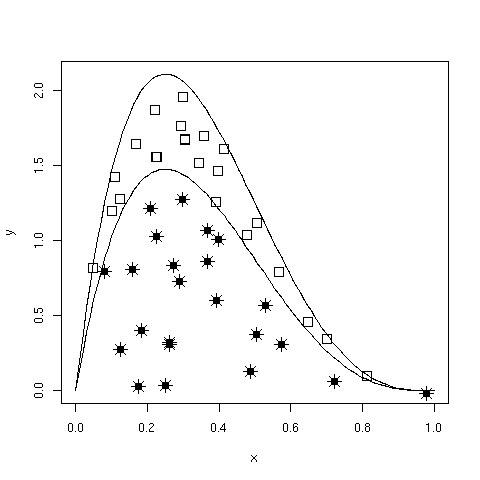
\includegraphics[scale=0.4]{envelope.png}
    \end{center}
    \caption{Rejection sampling of an unbounded form using an enveloping distribution.}
    \label{fig:unbound}
\end{figure}

\noindent This approach is useful, for example, in estimating the normalizing constant for posterior distributions.

If $f(x)$ has unbounded support (i.e. infinite tails), such as a Gaussian distribution, a bounding box is no longer appropriate. We must specify a majorizing (or, enveloping) function, $g(x)$, which implies:

\[
g(x) \ge  f(x) \qquad\forall x \in (-\infty,\infty)
\]

Having done this, we can now sample ${x_i}$ from $g(x)$ and accept or reject each of these values based upon $f(x_i)$. Specifically, for each draw $x_i$, we also draw a uniform random variate $u_i$ and accept $x_i$ if $u_i < f(x_i)/cg(x_i)$, where $c$ is a constant (Figure \ref{fig:unbound}). This approach is made more efficient by choosing an enveloping distribution that is ``close'' to the target distribution, thus maximizing the number of accepted points. Further improvement is gained by using optimized algorithms such as importance sampling which, as the name implies, samples more frequently from important areas of the distribution.

Rejection sampling is usually subject to declining performance as the dimension of the parameter space increases, so it is used less frequently than MCMC for evaluation of posterior distributions \citep{Gamerman:1997tb}.

%___________________________________________________________________________

\hypertarget{markov-chains}{}

\subsection{Markov Chains}

A Markov chain is a special type of \emph{stochastic process}. The standard definition of a stochastic process is an ordered collection of random variables:

\[
\{X_t:t \in T\}
\]

\noindent where $t$ is frequently (but not necessarily) a time index. If we think of $X_t$ as a state $X$ at time $t$, and invoke the following dependence condition on each state:

\[
Pr(X_{t+1}=x_{t+1} | X_t=x_t, X_{t-1}=x_{t-1},\ldots,X_0=x_0) = Pr(X_{t+1}=x_{t+1} | X_t=x_t)
\]

\noindent then the stochastic process is known as a Markov chain. This conditioning specifies that the future depends on the current state, but not past states. Thus, the Markov chain wanders about the state space, remembering only where it has just been in the last time step. The collection of transition probabilities is sometimes called a \emph{transition matrix} when dealing with discrete states, or more generally, a \emph{transition kernel}.

\noindent In the context of Markov chain Monte Carlo, it is useful to think of the Markovian property as ``mild non-independence''. MCMC allows us to indirectly generate independent samples from a particular posterior distribution.

%___________________________________________________________________________

\hypertarget{jargon-busting}{}

\subsubsection\*{Jargon-busting}

Before we move on, it is important to define some general properties of Markov chains. They are frequently encountered in the MCMC literature, and some will help us decide whether MCMC is producing a useful sample from the posterior.

\begin{itemize}
\item \emph{Homogeneity}: A Markov chain is homogeneous at step $t$ if the transition probabilities are independent of time $t$.
\item \emph{Irreducibility}: A Markov chain is irreducible if every state is accessible in one or more steps from any other state. That is, the chain contains no absorbing states. This implies that there is a non-zero probability of eventually reaching state $k$ from any other state in the chain.
\item \emph{Recurrence}: States which are visited repeatedly are \emph{recurrent}. If the expected time to return to a particular state is bounded, this is known as \emph{positive recurrence}, otherwise the recurrent state is \emph{null recurrent}. Further, a chain is \emph{Harris recurrent} when it visits all states $X \in S$ infinitely often in the limit as $t \to \infty$; this is an important characteristic when dealing with unbounded, continuous state spaces. Whenever a chain ends up in a closed, irreducible set of Harris recurrent states, it stays there forever and visits every state with probability one.
\item \emph{Stationarity}: A stationary Markov chain produces the same marginal distribution when multiplied by the transition kernel.  Thus, if $P$ is some $n \times n$ transition matrix:

\[{\bf \pi P} = {\bf \pi}\]

\noindent for Markov chain $\pi$. Thus, $\pi$ is no longer subscripted, and is referred to as the \emph{limiting distribution} of the chain. In MCMC, the chain explores the state space according to its limiting marginal distribution.
\item \emph{Ergodicity}: Ergodicity is an emergent property of Markov chains which are irreducible, positive Harris recurrent and aperiodic. Ergodicity is defined as:

\[
\lim_{n \to \infty} Pr^{(n)}(\theta_i \rightarrow \theta_j) = \pi(\theta) \quad \forall \theta_i, \theta_j \in \Theta
\]

\noindent or in words, after many steps the marginal distribution of the chain is the same at one step as at all other steps. This implies that our Markov chain, which we recall is dependent, can generate samples that are independent if we wait long enough between samples. If it means anything to you, ergodicity is the analogue of the strong law of large numbers for Markov chains. For example, take values $\theta_{i+1},\ldots,\theta_{i+n}$ from a chain that has reached an ergodic state. A statistic of interest can then be estimated by:

\[
\frac{1}{n}\sum_{j=i+1}^{i+n} h(\theta_j) \approx \int f(\theta) h(\theta) d\theta
\]

\end{itemize}

%___________________________________________________________________________

\hypertarget{reversible-markov-chains}{}

\subsection{Why MCMC Works: Reversible Markov Chains}

Markov chain Monte Carlo simulates a Markov chain for which some function of interest (\emph{e.g.} the joint distribution of the parameters of some model) is the unique, invariant limiting distribution. An invariant distribution with respect to some Markov chain with transition kernel $Pr(y \mid x)$ implies that:
\[
\int_x Pr(y \mid x) \pi(x) dx = \pi(y).
\]

Invariance is guaranteed for any \textbf{reversible} Markov chain. Consider a Markov chain in reverse sequence: $\{\theta^{(n)},\theta^{(n-1)},...,\theta^{(0)}\}$. This sequence is still Markovian, because:
\[
Pr(\theta^{(k)}=y \mid \theta^{(k+1)}=x,\theta^{(k+2)}=x_1,\ldots ) = Pr(\theta^{(k)}=y \mid \theta^{(k+1)}=x)
\]
Forward and reverse transition probabilities may be related through Bayes theorem:
\begin{eqnarray}
Pr(\theta^{(k)}=y \mid \theta^{(k+1)}=x) &=& \frac{Pr(\theta^{(k+1)}=x \mid \theta^{(k)}=y) Pr(\theta^{(k)}=y)}{Pr(\theta^{(k+1)}=x)} \nonumber \\
&=& \frac{Pr(\theta^{(k+1)}=x \mid \theta^{(k)}=y) \pi^{(k)}(y)}{\pi^{(k+1)}(x)} \nonumber
\end{eqnarray}

\[
\frac{Pr(\theta^{(k+1)}=x \mid \theta^{(k)}=y) \pi^{(k)}(y)}{\pi^{(k+1)}(x)}
\]

\noindent Though not homogeneous in general, $\pi$ becomes homogeneous if \textbf{Do you ever call the stationary distribution itself homogeneous?}:
\begin{itemize}
\item $n \rightarrow \infty$
\item $\pi^{(0)}=\pi$ for some $i < k$ \textbf{Is it meant to be $\pi^(i)$, and }
\end{itemize}

\noindent If this chain is homogeneous it is called reversible, because it satisfies the \textbf{detailed balance equation}:
\[
\pi(x)Pr(y \mid x) = \pi(y) Pr(x \mid y)
\]
Reversibility is important because it has the effect of balancing movement through the entire state space. When a Markov chain is reversible, $\pi$ is the unique, invariant, stationary distribution of that chain.
Hence, if $\pi$ is of interest, we need only find the reversible Markov chain for which $\pi$ is the limiting distribution. This is what MCMC does!

%___________________________________________________________________________

\hypertarget{gibbs-sampling}{}

\subsection{Gibbs Sampling}

The Gibbs sampler is the simplest and most prevalent MCMC algorithm. If a posterior has $k$ parameters to be estimated, we may condition each parameter on current values of the other $k-1$ parameters, and sample from the resultant distributional form (usually easier), and repeat this operation on the other parameters in turn. This procedure generates samples from the posterior distribution. Note that we have now combined Markov chains (conditional independence) and Monte Carlo techniques (estimation by simulation) to yield Markov chain Monte Carlo.

Here is a stereotypical Gibbs sampling algorithm:

\newcounter{lcount}
\begin{list}{\arabic{lcount}}
{\usecounter{lcount}}
\item Choose starting values for states (parameters): ${\bf \theta} = [\theta_1^{(0)},\theta_2^{(0)},\ldots,\theta_k^{(0)}]$
\item Initialize counter $j=1$
\item Draw the following values from each of the $k$ conditional distributions:
\begin{eqnarray*}
\theta_1^{(j)} &\sim& \pi(\theta_1 | \theta_2^{(j-1)},\theta_3^{(j-1)},\ldots,\theta_{k-1}^{(j-1)},\theta_k^{(j-1)}) \\
\theta_2^{(j)} &\sim& \pi(\theta_2 | \theta_1^{(j)},\theta_3^{(j-1)},\ldots,\theta_{k-1}^{(j-1)},\theta_k^{(j-1)}) \\
\theta_3^{(j)} &\sim& \pi(\theta_3 | \theta_1^{(j)},\theta_2^{(j)},\ldots,\theta_{k-1}^{(j-1)},\theta_k^{(j-1)}) \\
\vdots \\
\theta_{k-1}^{(j)} &\sim& \pi(\theta_{k-1} | \theta_1^{(j)},\theta_2^{(j)},\ldots,\theta_{k-2}^{(j)},\theta_k^{(j-1)}) \\
\theta_k^{(j)} &\sim& \pi(\theta_k | \theta_1^{(j)},\theta_2^{(j)},\theta_4^{(j)},\ldots,\theta_{k-2}^{(j)},\theta_{k-1}^{(j)})
\end{eqnarray*}
\item Increment $j$ and repeat until convergence occurs.
\end{list}

As we can see from the algorithm, each distribution is conditioned on the last iteration of its chain values, constituting a Markov chain as advertised. The Gibbs sampler has all of the important properties outlined in the previous section: it is aperiodic, homogeneous and ergodic. Once the sampler converges, all subsequent samples are from the target distribution. This convergence occurs at a geometric rate.

\hypertarget{the-metropolis-hastings-algorithm}{}

\subsection{The Metropolis-Hastings Algorithm}

The key to success in applying the Gibbs sampler to the estimation of Bayesian posteriors is being able to specify the form of the complete conditionals of ${\bf \theta}$. In fact, the algorithm cannot be implemented without them. Of course, the posterior conditionals cannot always be neatly specified. In contrast to the Gibbs algorithm, the Metropolis-Hastings algorithm generates candidate state transitions from an alternate distribution, and accepts or rejects each candidate probabilistically.

Let us first consider a simple Metropolis-Hastings algorithm for a single parameter, $\theta$. We will use a standard sampling distribution, referred to as the \emph{proposal distribution}, to produce candidate variables $q_t(\theta^{\prime} | \theta)$. That is, the generated value, $\theta^{\prime}$, is a \emph{possible} next value for $\theta$ at step $t+1$. We also need to be able to calculate the probability of moving back to the original value from the candidate, or $q_t(\theta | \theta^{\prime})$. These probabilistic ingredients are used to define an \emph{acceptance ratio}:

\[
a(\theta^{\prime},\theta) = \frac{q_t(\theta^{\prime} | \theta) \pi(\theta^{\prime})}{q_t(\theta | \theta^{\prime}) \pi(\theta)}
\]

\noindent The value of $\theta^{(t+1)}$ is then determined by:

\[
\theta^{(t+1)} = \left\{\begin{array}{l@{\quad \mbox{with prob.} \quad}l}\theta^{\prime} & \min(a(\theta^{\prime},\theta),1) \\ \theta^{(t)} & 1 - \min(a(\theta^{\prime},\theta),1) \end{array}\right.
\]

\noindent This transition kernel implies that movement is not guaranteed at every step. It only occurs if the suggested transition is likely based on the acceptance ratio.

A single iteration of the Metropolis-Hastings algorithm proceeds as follows:

\newcounter{lcount2}
\begin{list}{\arabic{lcount2}}
{\usecounter{lcount2}}
\item Sample $\theta^{\prime}$ from $q(\theta^{\prime} | \theta^{(t)})$.
\item Generate a Uniform[0,1] random variate $u$.
\item If $a(\theta^{\prime},\theta) > u$ then $\theta^{(t+1)} = \theta^{\prime}$, otherwise $\theta^{(t+1)} = \theta^{(t)}$.
\end{list}

\noindent The original form of the algorithm specified by Metropolis required that $q_t(\theta^{\prime} | \theta) = q_t(\theta | \theta^{\prime})$, which reduces $a(\theta^{\prime},\theta)$ to $\pi(\theta^{\prime})/\pi(\theta)$, but this is not necessary. In either case, the state moves to high-density points in the distribution with high probability, and to low-density points with low probability. After convergence, the Metropolis-Hastings algorithm describes the full target posterior density, so all points are recurrent.

%___________________________________________________________________________

\hypertarget{random-walk-metropolis-hastings}{}

\subsubsection\*{Random-walk Metropolis-Hastings}

A practical implementation of the Metropolis-Hastings algorithm makes use of a random-walk proposal. Recall that a random walk is a Markov chain that evolves according to:

\begin{eqnarray*}
\theta^{(t+1)} &=& \theta^{(t)} + \epsilon_t \\
\epsilon_t &\sim& f(\phi)
\end{eqnarray*}

As applied to the MCMC sampling, the random walk is used as a proposal distribution, whereby dependent proposals are generated according to:

\[
q(\theta^{\prime} | \theta^{(t)}) = f(\theta^{\prime} - \theta^{(t)}) = \theta^{(t)} + \epsilon_t
\]

Generally, the density generating $\epsilon_t$ is symmetric about zero, resulting in a symmetric chain. Chain symmetry implies that $q(\theta^{\prime} | \theta^{(t)}) = q(\theta^{(t)} | \theta^{\prime})$, which reduces the Metropolis-Hastings acceptance ratio to:

\[
a(\theta^{\prime},\theta) = \frac{\pi(\theta^{\prime})}{\pi(\theta)}
\]

The choice of the random walk distribution for $\epsilon_t$ is frequently a normal or Student's $t$ density, but it may be any distribution that generates an irreducible proposal chain.

An important consideration is the specification of the scale parameter for the random walk error distribution. Large values produce random walk steps that are highly exploratory, but tend to produce proposal values in the tails of the target distribution, potentially resulting in very small acceptance rates. Conversely, small values tend to be accepted more frequently, since they tend to produce proposals close to the current parameter value, but may result in chains that mix very slowly. Some simulation studies suggest optimal acceptance rates in the range of 20-50\%. It is often worthwhile to optimize the proposal variance by iteratively adjusting its value, according to observed acceptance rates early in the MCMC simulation \citep{Gamerman:1997tb}.



\section[Distributions]{Probability distributions}
\label{chap:distributions}
% Generated by Sphinx.
%\usepackage[utf8]{inputenc}
%\usepackage[T1]{fontenc}
%\usepackage{babel}
%\usepackage{times}
%\usepackage[Bjarne]{fncychap}


\pkg{PyMC} provides 35 built-in probability distributions. For each distribution, \pkg{PyMC} provides:
\begin{itemize}
    \item A function that evaluates its log-probability or log-density, for example \code{normal_like()}.
    \item A function that draws random variables, for example \code{rnormal()}.
    \item A function that computes the expectation associated with the distribution, for example \code{normal_expval()}.
    \item A \code{Stochastic} subclass generated from the distribution, for example \code{Normal}.
\end{itemize}

This Section~describes the likelihood functions of these distributions.
\index{pymc.distributions (module)}
\hypertarget{module-pymc.distributions}{}
%\declaremodule[pymc.distributions]{}{pymc.distributions}

\small

\subsection{Discrete distributions}
\index{bernoulli\_like() (in module pymc.distributions)}

\hypertarget{pymc.distributions.bernoulli_like}{}\begin{funcdesc}{bernoulli\_like}{x, p}
The Bernoulli distribution describes the probability of successes (x=1) and
failures (x=0).
\begin{gather}
\begin{split}f(x \mid p) = p^{x} (1-p)^{1-x}\end{split}\notag\\\begin{split}\end{split}\notag
\end{gather}\begin{description}
\item[Parameters] \leavevmode\begin{itemize}
\item {} 
\emph{x} : Series of successes (1) and failures (0). $x=0,1$

\item {} 
\emph{p} : Probability of success. $0 < p < 1$.

\end{itemize}

\item[Example] \leavevmode
\begin{Verbatim}[commandchars=@\[\]]
@PYGaQ[@textgreater[]@textgreater[]@textgreater[] ]bernoulli@_like(@PYGZlb[]@PYGaw[0],@PYGaw[1],@PYGaw[0],@PYGaw[1]@PYGZrb[], @PYGbe[.]@PYGaw[4])
@PYGaa[-2.8542325496673584]
\end{Verbatim}

\end{description}

\begin{notice}{note}{Note:}\begin{itemize}
\item {} 
$E(x)= p$

\item {} 
$Var(x)= p(1-p)$

\end{itemize}
\end{notice}
\end{funcdesc}
\index{binomial\_like() (in module pymc.distributions)}

\hypertarget{pymc.distributions.binomial_like}{}\begin{funcdesc}{binomial\_like}{x, n, p}
Binomial log-likelihood.  The discrete probability distribution of the
number of successes in a sequence of n independent yes/no experiments,
each of which yields success with probability p.
\begin{gather}
\begin{split}f(x \mid n, p) = \frac{n!}{x!(n-x)!} p^x (1-p)^{n-x}\end{split}\notag\\\begin{split}\end{split}\notag
\end{gather}\begin{description}
\item[Parameters] \leavevmode\begin{itemize}
\item {} 
\emph{x} : {[}int{]} Number of successes, \textgreater{} 0.

\item {} 
\emph{n} : {[}int{]} Number of Bernoulli trials, \textgreater{} x.

\item {} 
\emph{p} : Probability of success in each trial, $p \in [0,1]$.

\end{itemize}

\end{description}

\begin{notice}{note}{Note:}\begin{itemize}
\item {} 
$E(X)=np$

\item {} 
$Var(X)=np(1-p)$

\end{itemize}
\end{notice}
\end{funcdesc}
\index{categorical\_like() (in module pymc.distributions)}

\hypertarget{pymc.distributions.categorical_like}{}\begin{funcdesc}{categorical\_like}{x, p}
Categorical log-likelihood. The most general discrete distribution.
\begin{gather}
\begin{split}f(x=i \mid p) = p_i\end{split}\notag\\\begin{split}\end{split}\notag
\end{gather}
for $i \in 0 \ldots k-1$.
\begin{description}
\item[Parameters] \leavevmode\begin{itemize}
\item {} 
\emph{x} : {[}int{]} $x \in 0\ldots k-1$

\item {} 
\emph{p} : {[}float{]} $p > 0$, $\sum p = 1$

\end{itemize}

\end{description}
\end{funcdesc}
\index{discrete\_uniform\_like() (in module pymc.distributions)}

\hypertarget{pymc.distributions.discrete_uniform_like}{}\begin{funcdesc}{discrete\_uniform\_like}{x, lower, upper}
Discrete uniform log-likelihood.
\begin{gather}
\begin{split}f(x \mid lower, upper) = \frac{1}{upper-lower}\end{split}\notag\\\begin{split}\end{split}\notag
\end{gather}\begin{description}
\item[Parameters] \leavevmode\begin{itemize}
\item {} 
\emph{x} : {[}int{]} $lower \leq x \leq upper$

\item {} 
\emph{lower} : Lower limit.

\item {} 
\emph{upper} : Upper limit (upper \textgreater{} lower).

\end{itemize}

\end{description}
\end{funcdesc}
\index{geometric\_like() (in module pymc.distributions)}

\hypertarget{pymc.distributions.geometric_like}{}\begin{funcdesc}{geometric\_like}{x, p}
Geometric log-likelihood. The probability that the first success in a
sequence of Bernoulli trials occurs on the x'th trial.
\begin{gather}
\begin{split}f(x \mid p) = p(1-p)^{x-1}\end{split}\notag\\\begin{split}\end{split}\notag
\end{gather}\begin{description}
\item[Parameters] \leavevmode\begin{itemize}
\item {} 
\emph{x} : {[}int{]} Number of trials before first success (x \textgreater{} 0).

\item {} 
\emph{p} : Probability of success on an individual trial, $p \in [0,1]$

\end{itemize}

\end{description}

\begin{notice}{note}{Note:}\begin{itemize}
\item {} 
$E(X)=1/p$

\item {} 
$Var(X)=\frac{1-p}{p^2}$

\end{itemize}
\end{notice}
\end{funcdesc}
\index{hypergeometric\_like() (in module pymc.distributions)}

\hypertarget{pymc.distributions.hypergeometric_like}{}\begin{funcdesc}{hypergeometric\_like}{x, n, m, N}
Hypergeometric log-likelihood. Discrete probability distribution that
describes the number of successes in a sequence of draws from a finite
population without replacement.
\begin{gather}
\begin{split}f(x \mid n, m, N) = \frac{\binom{m}{x}\binom{N-m}{n-x}}{\binom{N}{n}}\end{split}\notag
\end{gather}\begin{description}
\item[Parameters] \leavevmode\begin{itemize}
\item {} 
\emph{x} : {[}int{]} Number of successes in a sample drawn from a population.

\item {} 
\emph{n} : {[}int{]} Size of sample drawn from the population.

\item {} 
\emph{m} : {[}int{]} Number of successes in the population.

\item {} 
\emph{N} : {[}int{]} Total number of units in the population.

\end{itemize}

\end{description}

\begin{notice}{note}{Note:}
$E(X) = \frac{n n}{N}$
\end{notice}
\end{funcdesc}
\index{negative\_binomial\_like() (in module pymc.distributions)}

\hypertarget{pymc.distributions.negative_binomial_like}{}\begin{funcdesc}{negative\_binomial\_like}{x, mu, alpha}
Negative binomial log-likelihood. The negative binomial distribution describes a
Poisson random variable whose rate parameter is gamma distributed. \pkg{PyMC}'s chosen
parameterization is based on this mixture interpretation.
\begin{gather}
\begin{split}f(x \mid \mu, \alpha) = \frac{\Gamma(x+\alpha)}{x! \Gamma(\alpha)} (\alpha/(\mu+\alpha))^\alpha (\mu/(\mu+\alpha))^x\end{split}\notag\\\begin{split}\end{split}\notag
\end{gather}\begin{description}
\item[Parameters] \leavevmode\begin{itemize}
\item {} 
\emph{x} : Input data (x \textgreater{} 0).

\item {} 
\emph{mu} : mu \textgreater{} 0

\item {} 
\emph{alpha} : alpha \textgreater{} 0

\end{itemize}

\end{description}

\begin{notice}{note}{Note:}\begin{itemize}
\item {} 
$E[x]=\mu$

\item {} 
In Wikipedia's parameterization,
$r=\alpha$
$p=\alpha/(\mu+\alpha)$
$\mu=r(1-p)/p$

\end{itemize}
\end{notice}
\end{funcdesc}
\index{poisson\_like() (in module pymc.distributions)}

\hypertarget{pymc.distributions.poisson_like}{}\begin{funcdesc}{poisson\_like}{x, mu}
Poisson log-likelihood. The Poisson is a discrete probability distribution.
It is often used to model the number of events occurring in a fixed period of
time when the times at which events occur are independent. The Poisson
distribution can be derived as a limiting case of the binomial distribution.
\begin{gather}
\begin{split}f(x \mid \mu) = \frac{e^{-\mu}\mu^x}{x!}\end{split}\notag\\\begin{split}\end{split}\notag
\end{gather}\begin{description}
\item[Parameters] \leavevmode\begin{itemize}
\item {} 
\emph{x} : {[}int{]} $x \in {0,1,2,...}$

\item {} 
\emph{mu} : Expected number of occurrences during the given interval, $\mu \geq 0$.

\end{itemize}

\end{description}

\begin{notice}{note}{Note:}\begin{itemize}
\item {} 
$E(x)=\mu$

\item {} 
$Var(x)=\mu$

\end{itemize}
\end{notice}
\end{funcdesc}


\subsection{Continuous distributions}
\index{beta\_like() (in module pymc.distributions)}

\hypertarget{pymc.distributions.beta_like}{}\begin{funcdesc}{beta\_like}{x, alpha, beta}
Beta log-likelihood. The conjugate prior for the parameter :math: \emph{p} of the binomial distribution.
\begin{gather}
\begin{split}f(x \mid \alpha, \beta) = \frac{\Gamma(\alpha + \beta)}{\Gamma(\alpha) \Gamma(\beta)} x^{\alpha - 1} (1 - x)^{\beta - 1}\end{split}\notag\\\begin{split}\end{split}\notag
\end{gather}\begin{description}
\item[Parameters] \leavevmode\begin{itemize}
\item {} 
\emph{x} : 0 \textless{} x \textless{} 1

\item {} 
\emph{alpha} : alpha \textgreater{} 0

\item {} 
\emph{beta} : beta \textgreater{} 0

\end{itemize}

\item[Example] \leavevmode
\begin{Verbatim}[commandchars=@\[\]]
@PYGaQ[@textgreater[]@textgreater[]@textgreater[] ]beta@_like(@PYGbe[.]@PYGaw[4],@PYGaw[1],@PYGaw[2])
@PYGaa[0.18232160806655884]
\end{Verbatim}

\end{description}

\begin{notice}{note}{Note:}\begin{itemize}
\item {} 
$E(X)=\frac{\alpha}{\alpha+\beta}$

\item {} 
$Var(X)=\frac{\alpha \beta}{(\alpha+\beta)^2(\alpha+\beta+1)}$

\end{itemize}
\end{notice}
\end{funcdesc}
\index{cauchy\_like() (in module pymc.distributions)}

\hypertarget{pymc.distributions.cauchy_like}{}\begin{funcdesc}{cauchy\_like}{x, alpha, beta}
Cauchy log-likelihood. The Cauchy distribution is also known as the
Lorentz or the Breit-Wigner distribution.
\begin{gather}
\begin{split}f(x \mid \alpha, \beta) = \frac{1}{\pi \beta [1 + (\frac{x-\alpha}{\beta})^2]}\end{split}\notag\\\begin{split}\end{split}\notag
\end{gather}\begin{description}
\item[Parameters] \leavevmode\begin{itemize}
\item {} 
\emph{alpha} : Location parameter.

\item {} 
\emph{beta} : Scale parameter \textgreater{} 0.

\end{itemize}

\end{description}

\begin{notice}{note}{Note:}\begin{itemize}
\item {} 
Mode and median are at alpha.

\end{itemize}
\end{notice}
\end{funcdesc}
\index{chi2\_like() (in module pymc.distributions)}

\hypertarget{pymc.distributions.chi2_like}{}\begin{funcdesc}{chi2\_like}{x, nu}
Chi-squared $\chi^2$ log-likelihood.
\begin{gather}
\begin{split}f(x \mid \nu) = \frac{x^{(\nu-2)/2}e^{-x/2}}{2^{\nu/2}\Gamma(\nu/2)}\end{split}\notag\\\begin{split}\end{split}\notag
\end{gather}\begin{description}
\item[Parameters] \leavevmode\begin{itemize}
\item {} 
\emph{x} : \textgreater{} 0

\item {} 
\emph{nu} : {[}int{]} Degrees of freedom ( nu \textgreater{} 0 )

\end{itemize}

\end{description}

\begin{notice}{note}{Note:}\begin{itemize}
\item {} 
$E(X)=\nu$

\item {} 
$Var(X)=2\nu$

\end{itemize}
\end{notice}
\end{funcdesc}
\index{degenerate\_like() (in module pymc.distributions)}

\hypertarget{pymc.distributions.degenerate_like}{}\begin{funcdesc}{degenerate\_like}{x, k}
Degenerate log-likelihood.
\begin{gather}
\begin{split}f(x \mid k) = \left\{ \begin{matrix} 1 \text{ if } x = k \\ 0 \text{ if } x \ne k\end{matrix} \right.\end{split}\notag\\\begin{split}\end{split}\notag
\end{gather}\begin{description}
\item[Parameters] \leavevmode\begin{itemize}
\item {} 
\emph{x} : Input value.

\item {} 
\emph{k} : Degenerate value.

\end{itemize}

\end{description}
\end{funcdesc}
\index{exponential\_like() (in module pymc.distributions)}

\hypertarget{pymc.distributions.exponential_like}{}\begin{funcdesc}{exponential\_like}{x, beta}
Exponential log-likelihood.

The exponential distribution is a special case of the gamma distribution
with alpha=1. It often describes the time until an event.
\begin{gather}
\begin{split}f(x \mid \beta) = \frac{1}{\beta}e^{-x/\beta}\end{split}\notag\\\begin{split}\end{split}\notag
\end{gather}\begin{description}
\item[Parameters] \leavevmode\begin{itemize}
\item {} 
\emph{x} : x \textgreater{} 0

\item {} 
\emph{beta} : Survival parameter (beta \textgreater{} 0).

\end{itemize}

\end{description}

\begin{notice}{note}{Note:}\begin{itemize}
\item {} 
$E(X) = \beta$

\item {} 
$Var(X) = \beta^2$

\end{itemize}
\end{notice}
\end{funcdesc}
\index{exponweib\_like() (in module pymc.distributions)}

\hypertarget{pymc.distributions.exponweib_like}{}\begin{funcdesc}{exponweib\_like}{x, alpha, k, loc=0, scale=1}
Exponentiated Weibull log-likelihood.

The exponentiated Weibull distribution is a generalization of the Weibull
family. Its value lies in being able to model monotone and non-monotone
failure rates.
\begin{gather}
\begin{split}f(x \mid \alpha,k,loc,scale)  & = \frac{\alpha k}{scale} (1-e^{-z^k})^{\alpha-1} e^{-z^k} z^{k-1} \\
z & = \frac{x-loc}{scale}\end{split}\notag\\\begin{split}\end{split}\notag
\end{gather}\begin{description}
\item[Parameters] \leavevmode\begin{itemize}
\item {} 
\emph{x} : x \textgreater{} 0

\item {} 
\emph{alpha} : Shape parameter

\item {} 
\emph{k} : k \textgreater{} 0

\item {} 
\emph{loc} : Location parameter

\item {} 
\emph{scale} : Scale parameter (scale \textgreater{} 0).

\end{itemize}

\end{description}
\end{funcdesc}
\index{gamma\_like() (in module pymc.distributions)}

\hypertarget{pymc.distributions.gamma_like}{}\begin{funcdesc}{gamma\_like}{x, alpha, beta}
Gamma log-likelihood.

Represents the sum of alpha exponentially distributed random variables, each
of which has mean beta.
\begin{gather}
\begin{split}f(x \mid \alpha, \beta) = \frac{\beta^{\alpha}x^{\alpha-1}e^{-\beta x}}{\Gamma(\alpha)}\end{split}\notag\\\begin{split}\end{split}\notag
\end{gather}\begin{description}
\item[Parameters] \leavevmode\begin{itemize}
\item {} 
\emph{x} : math:\emph{x ge 0}

\item {} 
\emph{alpha} : Shape parameter (alpha \textgreater{} 0).

\item {} 
\emph{beta} : Scale parameter (beta \textgreater{} 0).

\end{itemize}

\end{description}

\begin{notice}{note}{Note:}\begin{itemize}
\item {} 
$E(X) = \frac{\alpha}{\beta}$

\item {} 
$Var(X) = \frac{\alpha}{\beta^2}$

\end{itemize}
\end{notice}
\end{funcdesc}
\index{half\_normal\_like() (in module pymc.distributions)}

\hypertarget{pymc.distributions.half_normal_like}{}\begin{funcdesc}{half\_normal\_like}{x, tau}
Half-normal log-likelihood, a normal distribution with mean 0 limited
to the domain $x \in [0, \infty)$.
\begin{gather}
\begin{split}f(x \mid \tau) = \sqrt{\frac{2\tau}{\pi}}\exp\left\{ {\frac{-x^2 \tau}{2}}\right\}\end{split}\notag\\\begin{split}\end{split}\notag
\end{gather}\begin{description}
\item[Parameters] \leavevmode\begin{itemize}
\item {} 
\emph{x} : $x \ge 0$

\item {} 
\emph{tau} : tau \textgreater{} 0

\end{itemize}

\end{description}
\end{funcdesc}
\index{hypergeometric\_like() (in module pymc.distributions)}

\begin{funcdesc}{hypergeometric\_like}{x, n, m, N}
Hypergeometric log-likelihood. Discrete probability distribution that
describes the number of successes in a sequence of draws from a finite
population without replacement.
\begin{gather}
\begin{split}f(x \mid n, m, N) = \frac{\binom{m}{x}\binom{N-m}{n-x}}{\binom{N}{n}}\end{split}\notag
\end{gather}\begin{description}
\item[Parameters] \leavevmode\begin{itemize}
\item {} 
\emph{x} : {[}int{]} Number of successes in a sample drawn from a population.

\item {} 
\emph{n} : {[}int{]} Size of sample drawn from the population.

\item {} 
\emph{m} : {[}int{]} Number of successes in the population.

\item {} 
\emph{N} : {[}int{]} Total number of units in the population.

\end{itemize}

\end{description}

\begin{notice}{note}{Note:}
$E(X) = \frac{n n}{N}$
\end{notice}
\end{funcdesc}
\index{inverse\_gamma\_like() (in module pymc.distributions)}

\hypertarget{pymc.distributions.inverse_gamma_like}{}\begin{funcdesc}{inverse\_gamma\_like}{x, alpha, beta}
Inverse gamma log-likelihood, the reciprocal of the gamma distribution.
\begin{gather}
\begin{split}f(x \mid \alpha, \beta) = \frac{\beta^{\alpha}}{\Gamma(\alpha)} x^{-\alpha - 1} \exp\left(\frac{-\beta}{x}\right)\end{split}\notag\\\begin{split}\end{split}\notag
\end{gather}\begin{description}
\item[Parameters] \leavevmode\begin{itemize}
\item {} 
\emph{x} : x \textgreater{} 0

\item {} 
\emph{alpha} : Shape parameter (alpha \textgreater{} 0).

\item {} 
\emph{beta} : Scale parameter (beta \textgreater{} 0).

\end{itemize}

\end{description}

\begin{notice}{note}{Note:}
$E(X)=\frac{\beta}{\alpha-1}$  for $\alpha > 1$
$Var(X)=\frac{\beta^2}{(\alpha-1)^2(\alpha)}$  for $\alpha > 2$
\end{notice}
\end{funcdesc}
\index{laplace\_like() (in module pymc.distributions)}

\hypertarget{pymc.distributions.laplace_like}{}\begin{funcdesc}{laplace\_like}{x, mu, tau}
Laplace (double exponential) log-likelihood.

The Laplace (or double exponential) distribution describes the
difference between two independent, identically distributed exponential
events. It is often used as a heavier-tailed alternative to the normal.
\begin{gather}
\begin{split}f(x \mid \mu, \tau) = \frac{\tau}{2}e^{-\tau |x-\mu|}\end{split}\notag\\\begin{split}\end{split}\notag
\end{gather}\begin{description}
\item[Parameters] \leavevmode\begin{itemize}
\item {} 
\emph{x} : $-\infty < x < \infty$

\item {} 
\emph{mu} : Location parameter :math: \emph{-infty \textless{} mu \textless{} infty}

\item {} 
\emph{tau} : Scale parameter $\tau > 0$

\end{itemize}

\end{description}

\begin{notice}{note}{Note:}\begin{itemize}
\item {} 
$E(X) = \mu$

\item {} 
$Var(X) = \frac{2}{\tau^2}$

\end{itemize}
\end{notice}
\end{funcdesc}
\index{logistic\_like() (in module pymc.distributions)}

\hypertarget{pymc.distributions.logistic_like}{}\begin{funcdesc}{logistic\_like}{x, mu, tau}
Logistic log-likelihood.

The logistic distribution is often used as a growth model; for example,
populations, markets. Resembles a heavy-tailed normal distribution.
\begin{gather}
\begin{split}f(x \mid \mu, tau) = \frac{\tau \exp(-\tau[x-\mu])}{[1 + \exp(-\tau[x-\mu])]^2}\end{split}\notag\\\begin{split}\end{split}\notag
\end{gather}\begin{description}
\item[Parameters] \leavevmode\begin{itemize}
\item {} 
\emph{x} : $-\infty < x < \infty$

\item {} 
\emph{mu} : Location parameter $-\infty < mu < \infty$

\item {} 
\emph{tau} : Scale parameter (tau \textgreater{} 0)

\end{itemize}

\end{description}

\begin{notice}{note}{Note:}\begin{itemize}
\item {} 
$E(X) = \mu$

\item {} 
$Var(X) = \frac{\pi^2}{3\tau^2}$

\end{itemize}
\end{notice}
\end{funcdesc}
\index{lognormal\_like() (in module pymc.distributions)}

\hypertarget{pymc.distributions.lognormal_like}{}\begin{funcdesc}{lognormal\_like}{x, mu, tau}
Log-normal log-likelihood. Distribution of any random variable whose
logarithm is normally distributed. A variable might be modeled as
log-normal if it can be thought of as the multiplicative product of many
small independent factors.
\begin{gather}
\begin{split}f(x \mid \mu, \tau) = \sqrt{\frac{\tau}{2\pi}}\frac{
\exp\left\{ -\frac{\tau}{2} (\ln(x)-\mu)^2 \right\}}{x}\end{split}\notag\\\begin{split}\end{split}\notag
\end{gather}\begin{description}
\item[Parameters] \leavevmode\begin{itemize}
\item {} 
\emph{x} : x \textgreater{} 0

\item {} 
\emph{mu} : Location parameter.

\item {} 
\emph{tau} : Scale parameter (tau \textgreater{} 0).

\end{itemize}

\end{description}

\begin{notice}{note}{Note:}
$E(X)=e^{\mu+\frac{1}{2\tau}}$
$Var(X)=(e^{1/\tau}-1)e^{2\mu+\frac{1}{\tau}}$
\end{notice}
\end{funcdesc}
\index{normal\_like() (in module pymc.distributions)}

\hypertarget{pymc.distributions.normal_like}{}\begin{funcdesc}{normal\_like}{x, mu, tau}
Normal log-likelihood.
\begin{gather}
\begin{split}f(x \mid \mu, \tau) = \sqrt{\frac{\tau}{2\pi}} \exp\left\{ -\frac{\tau}{2} (x-\mu)^2 \right\}\end{split}\notag\\\begin{split}\end{split}\notag
\end{gather}\begin{description}
\item[Parameters] \leavevmode\begin{itemize}
\item {} 
\emph{x} : Input data.

\item {} 
\emph{mu} : Mean of the distribution.

\item {} 
\emph{tau} : Precision of the distribution, which corresponds to $1/\sigma^2$ (tau \textgreater{} 0).

\end{itemize}

\end{description}

\begin{notice}{note}{Note:}\begin{itemize}
\item {} 
$E(X) = \mu$

\item {} 
$Var(X) = 1/\tau$

\end{itemize}
\end{notice}
\end{funcdesc}
\index{skew\_normal\_like() (in module pymc.distributions)}

\hypertarget{pymc.distributions.skew_normal_like}{}\begin{funcdesc}{skew\_normal\_like}{x, mu, tau, alpha}
Azzalini's skew-normal log-likelihood
\begin{gather}
\begin{split}f(x \mid \mu, \tau, \alpha) = 2 \Phi((x-\mu)\sqrt{\tau}\alpha) \phi(x,\mu,\tau)\end{split}\notag\\\begin{split}\end{split}\notag
\end{gather}
where :math: Phi is the normal CDF and :math: phi is the normal PDF.
\begin{description}
\item[Parameters] \leavevmode\begin{itemize}
\item {} 
\emph{x} : Input data.

\item {} 
\emph{mu} : Mean of the distribution.

\item {} 
\emph{tau} : Precision of the distribution (\textgreater{} 0).

\item {} 
\emph{alpha} : Shape parameter of the distribution.

\end{itemize}

\end{description}

\begin{notice}{note}{Note:}
See \href{http://azzalini.stat.unipd.it/SN/}{http://azzalini.stat.unipd.it/SN/}
\end{notice}
\end{funcdesc}
\index{t\_like() (in module pymc.distributions)}

\hypertarget{pymc.distributions.t_like}{}\begin{funcdesc}{t\_like}{x, nu}
Student's T log-likelihood. Describes a zero-mean normal variable whose precision is
gamma distributed. Alternatively, describes the mean of several zero-mean normal
random variables divided by their sample standard deviation.
\begin{gather}
\begin{split}f(x \mid \nu) = \frac{\Gamma(\frac{\nu+1}{2})}{\Gamma(\frac{\nu}{2}) \sqrt{\nu\pi}} \left( 1 + \frac{x^2}{\nu} \right)^{-\frac{\nu+1}{2}}\end{split}\notag\\\begin{split}\end{split}\notag
\end{gather}\begin{description}
\item[Parameters] \leavevmode\begin{itemize}
\item {} 
\emph{x} : Input data.

\item {} 
\emph{nu} : Degrees of freedom.

\end{itemize}

\end{description}
\end{funcdesc}
\index{truncnorm\_like() (in module pymc.distributions)}

\hypertarget{pymc.distributions.truncnorm_like}{}\begin{funcdesc}{truncnorm\_like}{x, mu, tau, a, b}
Truncated normal log-likelihood.
\begin{gather}
\begin{split}f(x \mid \mu, \tau, a, b) = \frac{\phi(\frac{x-\mu}{\sigma})} {\Phi(\frac{b-\mu}{\sigma}) - \Phi(\frac{a-\mu}{\sigma})},\end{split}\notag\\\begin{split}\end{split}\notag
\end{gather}
where $\sigma^2=1/\tau$, \emph{phi} is the standard normal PDF and \emph{Phi} is the standard normal CDF.
\begin{description}
\item[Parameters] \leavevmode\begin{itemize}
\item {} 
\emph{x} : Input data.

\item {} 
\emph{mu} : Mean of the distribution.

\item {} 
\emph{tau} : Precision of the distribution, which corresponds to 1/sigma**2 (tau \textgreater{} 0).

\item {} 
\emph{a} : Left bound of the distribution.

\item {} 
\emph{b} : Right bound of the distribution.

\end{itemize}

\end{description}
\end{funcdesc}
\index{uniform\_like() (in module pymc.distributions)}

\hypertarget{pymc.distributions.uniform_like}{}\begin{funcdesc}{uniform\_like}{x, lower, upper}
Uniform log-likelihood.
\begin{gather}
\begin{split}f(x \mid lower, upper) = \frac{1}{upper-lower}\end{split}\notag\\\begin{split}\end{split}\notag
\end{gather}\begin{description}
\item[Parameters] \leavevmode\begin{itemize}
\item {} 
\emph{x} : $lower \leq x \leq upper$

\item {} 
\emph{lower} : Lower limit.

\item {} 
\emph{upper} : Upper limit (upper \textgreater{} lower).

\end{itemize}

\end{description}
\end{funcdesc}
\index{von\_mises\_like() (in module pymc.distributions)}

\hypertarget{pymc.distributions.von_mises_like}{}\begin{funcdesc}{von\_mises\_like}{x, mu, kappa}
von Mises log-likelihood.
\begin{gather}
\begin{split}f(x \mid \mu, k) = \frac{e^{k \cos(x - \mu)}}{2 \pi I_0(k)}\end{split}\notag\\\begin{split}\end{split}\notag
\end{gather}
where \emph{I\_0} is the modified Bessel function of order 0.
\begin{description}
\item[Parameters] \leavevmode\begin{itemize}
\item {} 
\emph{x} : Input data.

\item {} 
\emph{mu} : Mean of the distribution.

\item {} 
\emph{kappa} : Dispersion of the distribution

\end{itemize}

\end{description}

\begin{notice}{note}{Note:}\begin{itemize}
\item {} 
$E(X) = \mu$

\end{itemize}
\end{notice}
\end{funcdesc}
\index{weibull\_like() (in module pymc.distributions)}

\hypertarget{pymc.distributions.weibull_like}{}\begin{funcdesc}{weibull\_like}{x, alpha, beta}
Weibull log-likelihood
\begin{gather}
\begin{split}f(x \mid \alpha, \beta) = \frac{\alpha x^{\alpha - 1}
\exp(-(\frac{x}{\beta})^{\alpha})}{\beta^\alpha}\end{split}\notag\\\begin{split}\end{split}\notag
\end{gather}\begin{description}
\item[Parameters] \leavevmode\begin{itemize}
\item {} 
\emph{x} : $x \ge 0$

\item {} 
\emph{alpha} : alpha \textgreater{} 0

\item {} 
\emph{beta} : beta \textgreater{} 0

\end{itemize}

\end{description}

\begin{notice}{note}{Note:}\begin{itemize}
\item {} 
$E(x)=\beta \Gamma(1+\frac{1}{\alpha})$

\item {} 
$Var(x)=\beta^2 \Gamma(1+\frac{2}{\alpha} - \mu^2)$

\end{itemize}
\end{notice}
\end{funcdesc}


\subsection{Multivariate discrete distributions}
\index{multivariate\_hypergeometric\_like() (in module pymc.distributions)}

\hypertarget{pymc.distributions.multivariate_hypergeometric_like}{}\begin{funcdesc}{multivariate\_hypergeometric\_like}{x, m}
The multivariate hypergeometric describes the probability of drawing x{[}i{]}
elements of the ith category, when the number of items in each category is
given by m.
\begin{gather}
\begin{split}\frac{\prod_i \binom{m_i}{x_i}}{\binom{N}{n}}\end{split}\notag\\\begin{split}\end{split}\notag
\end{gather}
where $N = \sum_i m_i$ and $n = \sum_i x_i$.
\begin{description}
\item[Parameters] \leavevmode\begin{itemize}
\item {} 
\emph{x} : {[}int sequence{]} Number of draws from each category, (x \textless{} m).

\item {} 
\emph{m} : {[}int sequence{]} Number of items in each categoy.

\end{itemize}

\end{description}
\end{funcdesc}
\index{multinomial\_like() (in module pymc.distributions)}

\hypertarget{pymc.distributions.multinomial_like}{}\begin{funcdesc}{multinomial\_like}{x, n, p}
Multinomial log-likelihood. Generalization of the binomial
distribution, but instead of each trial resulting in ``success'' or
``failure'', each one results in exactly one of some fixed finite number k
of possible outcomes over n independent trials. `x{[}i{]}' indicates the number
of times outcome number i was observed over the n trials.
\begin{gather}
\begin{split}f(x \mid n, p) = \frac{n!}{\prod_{i=1}^k x_i!} \prod_{i=1}^k p_i^{x_i}\end{split}\notag\\\begin{split}\end{split}\notag
\end{gather}\begin{description}
\item[Parameters] \leavevmode\begin{description}
\item[x] \leavevmode{[}(ns, k) int{]}
Random variable indicating the number of time outcome i is 
observed. $\sum_{i=1}^k x_i=n$, $x_i \ge 0$.

\item[n] \leavevmode{[}int{]}
Number of trials.

\item[p] \leavevmode{[}(k,) {]}
Probability of each one of the different outcomes.
$\sum_{i=1}^k p_i = 1)$, $p_i \ge 0$.

\end{description}

\end{description}

\begin{notice}{note}{Note:}\begin{itemize}
\item {} 
$E(X_i)=n p_i$

\item {} 
$Var(X_i)=n p_i(1-p_i)$

\item {} 
$Cov(X_i,X_j) = -n p_i p_j$

\end{itemize}
\end{notice}
\end{funcdesc}


\subsection{Multivariate continuous distributions}
\index{dirichlet\_like() (in module pymc.distributions)}

\hypertarget{pymc.distributions.dirichlet_like}{}\begin{funcdesc}{dirichlet\_like}{x, theta}
Dirichlet log-likelihood.

This is a multivariate continuous distribution.
\begin{gather}
\begin{split}f(\mathbf{x}) = \frac{\Gamma(\sum_{i=1}^k \theta_i)}{\prod \Gamma(\theta_i)}\prod_{i=1}^{k-1} x_i^{\theta_i - 1}\cdot\left(1-\sum_{i=1}^{k-1}x_i\right)^\theta_k\end{split}\notag\\\begin{split}\end{split}\notag
\end{gather}\begin{description}
\item[Parameters] \leavevmode\begin{description}
\item[x] \leavevmode{[}(n, k-1) array {]}
Array of shape (n, k-1) where \emph{n} is the number of samples 
and \emph{k} the dimension. 
$0 < x_i < 1$,  $\sum_{i=1}^{k-1} x_i < 1$
\item[theta] \leavevmode{[}array{]}
An (n,k) or (1,k) array \textgreater{} 0.

\end{description}

\end{description}

\begin{notice}{note}{Note:}
Only the first \emph{k-1} elements of \emph{x} are expected. Can be used as a parent of Multinomial and Categorical
nevertheless.
\end{notice}
\end{funcdesc}
\index{inverse\_wishart\_like() (in module pymc.distributions)}

\hypertarget{pymc.distributions.inverse_wishart_like}{}\begin{funcdesc}{inverse\_wishart\_like}{X, n, Tau}
Inverse Wishart log-likelihood. The inverse Wishart distribution is the conjugate
prior for the covariance matrix of a multivariate normal distribution.
\begin{gather}
\begin{split}f(X \mid n, T) = \frac{{\mid T \mid}^{n/2}{\mid X \mid}^{(n-k-1)/2} \exp\left\{ -\frac{1}{2} Tr(TX^{-1}) \right\}}{2^{nk/2} \Gamma_p(n/2)}\end{split}\notag\\\begin{split}\end{split}\notag
\end{gather}
where $k$ is the rank of X.
\begin{description}
\item[Parameters] \leavevmode\begin{itemize}
\item {} 
\emph{X} : Symmetric, positive definite matrix.

\item {} 
\emph{n} : {[}int{]} Degrees of freedom (n \textgreater{} 0).

\item {} 
\emph{Tau} : Symmetric and positive definite matrix.

\end{itemize}

\end{description}

\begin{notice}{note}{Note:}
Step method MatrixMetropolis will preserve the symmetry of Wishart variables.
\end{notice}
\end{funcdesc}
\index{mv\_normal\_like() (in module pymc.distributions)}

\hypertarget{pymc.distributions.mv_normal_like}{}\begin{funcdesc}{mv\_normal\_like}{x, mu, tau}
Multivariate normal log-likelihood
\begin{gather}
\begin{split}f(x \mid \pi, T) = \frac{|T|^{1/2}}{(2\pi)^{1/2}} \exp\left\{ -\frac{1}{2} (x-\mu)^{\prime}T(x-\mu) \right\}\end{split}\notag\\\begin{split}\end{split}\notag
\end{gather}\begin{description}
\item[Parameters] \leavevmode\begin{itemize}
\item {} 
\emph{x} : (n,k)

\item {} 
\emph{mu} : (k) Location parameter sequence.

\item {} 
\emph{Tau} : (k,k) Positive definite precision matrix.

\end{itemize}

\end{description}


\strong{See Also:}


\hyperlink{pymc.distributions.mv_normal_chol_like}{\code{mv\_normal\_chol\_like()}}, \hyperlink{pymc.distributions.mv_normal_cov_like}{\code{mv\_normal\_cov\_like()}}


\end{funcdesc}
\index{mv\_normal\_chol\_like() (in module pymc.distributions)}

\hypertarget{pymc.distributions.mv_normal_chol_like}{}\begin{funcdesc}{mv\_normal\_chol\_like}{x, mu, sig}
Multivariate normal log-likelihood.
\begin{gather}
\begin{split}f(x \mid \pi, \sigma) = \frac{1}{(2\pi)^{1/2}|\sigma|)} \exp\left\{ -\frac{1}{2} (x-\mu)^{\prime}(\sigma \sigma^{\prime})^{-1}(x-\mu) \right\}\end{split}\notag\\\begin{split}\end{split}\notag
\end{gather}\begin{description}
\item[Parameters] \leavevmode\begin{itemize}
\item {} 
\emph{x} : (n,k)

\item {} 
\emph{mu} : (k) Location parameter.

\item {} 
\emph{sigma} : (k,k) Lower triangular matrix.

\end{itemize}

\end{description}


\strong{See Also:}


\hyperlink{pymc.distributions.mv_normal_like}{\code{mv\_normal\_like()}}, \hyperlink{pymc.distributions.mv_normal_cov_like}{\code{mv\_normal\_cov\_like()}}


\end{funcdesc}
\index{mv\_normal\_cov\_like() (in module pymc.distributions)}

\hypertarget{pymc.distributions.mv_normal_cov_like}{}\begin{funcdesc}{mv\_normal\_cov\_like}{x, mu, C}
Multivariate normal log-likelihood parameterized by a covariance 
matrix.
\begin{gather}
\begin{split}f(x \mid \pi, C) = \frac{1}{(2\pi|C|)^{1/2}} \exp\left\{ -\frac{1}{2} (x-\mu)^{\prime}C^{-1}(x-\mu) \right\}\end{split}\notag\\\begin{split}\end{split}\notag
\end{gather}\begin{description}
\item[Parameters] \leavevmode\begin{itemize}
\item {} 
\emph{x} : (n,k)

\item {} 
\emph{mu} : (k) Location parameter.

\item {} 
\emph{C} : (k,k) Positive definite covariance matrix.

\end{itemize}

\end{description}


\strong{See Also:}


\hyperlink{pymc.distributions.mv_normal_like}{\code{mv\_normal\_like()}}, \hyperlink{pymc.distributions.mv_normal_chol_like}{\code{mv\_normal\_chol\_like()}}


\end{funcdesc}
\index{wishart\_like() (in module pymc.distributions)}

\hypertarget{pymc.distributions.wishart_like}{}\begin{funcdesc}{wishart\_like}{X, n, Tau}
Wishart log-likelihood. The Wishart distribution is the probability
distribution of the maximum-likelihood estimator (MLE) of the precision
matrix of a multivariate normal distribution. If Tau=1, the distribution
is identical to the chi-square distribution with n degrees of freedom.

For an alternative parameterization based on $C=T{-1}$, see
\emph{wishart\_cov\_like}.
\begin{gather}
\begin{split}f(X \mid n, T) = {\mid T \mid}^{n/2}{\mid X \mid}^{(n-k-1)/2} \exp\left\{ -\frac{1}{2} Tr(TX) \right\}\end{split}\notag\\\begin{split}\end{split}\notag
\end{gather}
where $k$ is the rank of X.
\begin{description}
\item[Parameters] \leavevmode\begin{description}
\item[X] \leavevmode{[}matrix{]}
Symmetric, positive definite.

\item[n] \leavevmode{[}int{]}
Degrees of freedom, \textgreater{} 0.

\item[Tau] \leavevmode{[}matrix{]}
Symmetric and positive definite

\end{description}

\end{description}

\begin{notice}{note}{Note:}
Step method MatrixMetropolis will preserve the symmetry of Wishart variables.
\end{notice}
\end{funcdesc}
\index{wishart\_cov\_like() (in module pymc.distributions)}

\hypertarget{pymc.distributions.wishart_cov_like}{}\begin{funcdesc}{wishart\_cov\_like}{X, n, C}
Wishart log-likelihood. The Wishart distribution is the probability
distribution of the maximum-likelihood estimator (MLE) of the covariance
matrix of a multivariate normal distribution. If C=1, the distribution
is identical to the chi-square distribution with n degrees of freedom.

For an alternative parameterization based on $T=C{-1}$, see
\emph{wishart\_like}.
\begin{gather}
\begin{split}f(X \mid n, C) = {\mid C^{-1} \mid}^{n/2}{\mid X \mid}^{(n-k-1)/2} \exp\left\{ -\frac{1}{2} Tr(C^{-1}X) \right\}\end{split}\notag\\\begin{split}\end{split}\notag
\end{gather}
where $k$ is the rank of X.
\begin{description}
\item[Parameters] \leavevmode\begin{description}
\item[X] \leavevmode{[}matrix{]}
Symmetric, positive definite.

\item[n] \leavevmode{[}int{]}
Degrees of freedom, \textgreater{} 0.

\item[C] \leavevmode{[}matrix{]}
Symmetric and positive definite

\end{description}

\end{description}
\end{funcdesc}
\normalsize


\newpage

\nocite{Bernardo:1992fk}
\nocite{r} 
\nocite{jags} 
\nocite{winbugs}
\nocite{hbc} 
\bibliography{pymc}

\end{document}

